\documentclass[10pt,spanish,a4paper,notitlepage]{article}
\usepackage[spanish,es-tabla]{babel}  	% Traduce los textos a castellano
\usepackage[utf8]{inputenc}
\usepackage{units}
\usepackage{fancyhdr}
\usepackage{anysize}
\usepackage{float}
\usepackage[dvipsnames]{xcolor}
\usepackage{abstract} % paquete para el resumen del articulo
\usepackage[square,sort,comma,numbers]{natbib}
\usepackage{graphicx}
\usepackage{tablefootnote} % para agregar notas al pie de pagina en las tablas
\usepackage{amsmath} % para agregar acentos a las variables matemáticas, como por ej ^ para indicar el valor pico
\usepackage{hyperref} % para agregar url
\usepackage[bottom]{footmisc} % para que las footnote estén al final de la hoja y no cuando termina el texto
\usepackage{multirow}
\usepackage{amssymb}

\usepackage[europeanvoltages]{circuitikz}

\setcitestyle{square} %cambio las citas a [] en lugar de ()

% todo lo que sigue es para poner links que se les pueda hacer click
\usepackage{xcolor}
\usepackage[normalem]{ulem}
\usepackage{hyperref}
\hypersetup{colorlinks,urlcolor=blue}


\setlength{\headheight}{33pt} 

\makeatletter
\DeclareUrlCommand\ULurl@@{%
  \def\UrlFont{\ttfamily\color{blue}}%
  \def\UrlLeft{\uline\bgroup}%
  \def\UrlRight{\egroup}}
\def\ULurl@#1{\hyper@linkurl{\ULurl@@{#1}}{#1}}
\DeclareRobustCommand*\ULurl{\hyper@normalise\ULurl@}
\makeatother

%---------------------------------------Configuraciones de pagina----------------------------------------------
\marginsize{2.5cm}{2.5cm}{1cm}{1cm}

\pagestyle{fancy}
\fancyhf{}
\lhead{
86.06 - \textsc{Circuitos Electrónicos}\\ 
1\textsuperscript{er} Cuatrimestre de 2016
}
\rhead{
\includegraphics[width=3cm]{includes/FIUBA_ALTA.jpg}}
\rfoot{Página \thepage}

%------------------------------ graphicx ----------------------------------
%
% Todas las imagenes estan en el directorio tp-img:
%
\newcommand{\imgdir}{includes}
\graphicspath{{\imgdir/}}
%


%------------------------- Inicio del documento ---------------------------

\begin{document}

\begin{titlepage}

\thispagestyle{empty}

\begin{center}

\includegraphics[width=5cm]{fiuba}\\
\large{\textsc{Universidad de Buenos Aires}}\\
\large{\textsc{Facultad De Ingeniera}}\\
\small{2016 - 1\textsuperscript{er} Cuatrimestre}
\end{center}

\vfill
\begin{center}
\Large{\underline{86.06 - \textsc{Circuitos Electrónicos}}}
\end{center}

\vfill

\begin{tabbing}
\hspace{2cm}\=\+TRABAJO DE LABORATORIO 2\\
	Etapas con transistores discretos\\
	\today\\
\\
	INTEGRANTES:\hspace{-1cm}\=\+\hspace{1cm}\=\hspace{6cm}\=\\
		Bruno, Nicolas	\>\> 95191\\
			\>\footnotesize{$<$nicoo.24@hotmail.com$>$}\\
		Hagata, Juan Pablo	\>\> 93856\\
			\>\footnotesize{$<$jpablo.hagata@gmail.com$>$}\\
		Vazquez, Matias	\>\> 91523\\
			\>\footnotesize{$<$mfvazquezfiuba@gmail.com$>$}\\
\end{tabbing}

\vfill

\hrule
\vspace{0.2cm}

\end{titlepage}

%
% Hago que las paginas se comiencen a contar a partir de aqui
%
\setcounter{page}{1}

%
% Pongo el indice en una pagina aparte:
%
\tableofcontents
\newpage

\section{Introducción}

Se analizará el funcionamiento de un amplificador de una etapa ``Emisor
común"\ / ``Source común" o de uno ``Base común"\ / ``Gate común". Se
buscarán sus parámetros característicos y la influencia en su
funcionamiento al agregar un seguidor en la entrada.
Por ultimo se analizará el funcionamiento de un oscilador.

\section{Etapa amplificadora con un transistor}

\subsection{Justificación del diseño}

Obtenga una configuración que brinde 
$R_i = 10\,\unit{k\Omega}$, $|A_v| = 50$.\\

Para lograr estas especificaciones se tuvieron en cuenta tanto la
configuración como la tecnología a utilizar. Debido a la alta impedancia de
entrada que se requiere, se optó por usar transistores de tipo FET, eligiendo
utilizar MOSFET, ya que los TBJ no presentan una impedancia de entrada de la magnitud requerida en ninguna configuración. Para lograr la amplificación pedida se decidió utilizar al
MOSFET en configuración source común. Esto se debe a que si se lo utilizara en
configuración gate común se tendría una impedancia de entrada de valor
$\frac{1}{g_m}$ que apenas alcanza los cientos de ohms, mientras que si se lo
utilizara en drain común, la amplificación seria menor a 1.


\begin{figure}[H]
\centering
\begin{circuitikz}[]\shorthandoff{>}
\draw 
(6,4.27) node[nigfete](nmos){}

(0,0) to [sV, l=$v_s$] (0,2) 
to [R, l=$R_s$] (0,4)
to [short] (1.5,4)
to [C, l=$C_{A1}$] (3,4)
to [short] (3,5)
to [R, l=$R_{G1}$] (3,7)
to [short] (6,7)
to [R, l=$R_D$] (nmos.D)

(3,0) to [R, l=$R_{G2}$] (3,4) 
to [short, *-] (nmos.G)
(nmos.S) to [R, l=$R_S$] (6,0)

(6,3) to [short, *-] (8,3) 
to [C, l=$C_S$] (8,0)

(6,5) to [short, *-] (8,5)
to [C, l=$C_{A2}$] (11,5)
to [R, l=$R_L$] (11,0)
to [short, -*] (8,0)
to [short, -*] (6,0)
to [short, -*] (3,0)
to [short] (0,0)

(4.5, 7) to [short, -o] (4.5,7.5)  node[anchor=south] {$V_{DD}$}

(6,0) node[ground]{}

(nmos.G) node[anchor=south] {$G$}
(nmos.D) node[anchor=east] {$D$}
(nmos.S) node[anchor=west] {$S$}

(1,4) to [open, v=$v_i$] (1,0)
(10,5) to [open, v=$v_o$] (10,0)
;\end{circuitikz}
\caption{Circuito de la etapa amplificadora}
\label{fig:A_circuito}
\end{figure}

\begin{table}[H]
    \centering
    \begin{tabular}{|c|c|c|c|c|c|c|c|c|} %aca pones la cantidad de columnas, te faltaba 1. la c indica que esta centrado el dato en su celda y las | son cada linea vertical de la tabla
    \hline
    $R_{G1}$ & $R_{G2}$ & $R_{s}$ & $R_{D}$ & $R_{S}$ & $R_{L}$ & $C_{A1}$ & $C_{S}$ & $V_{DD}$  \\ \hline
    $820\,\unit{k\Omega}$ & $100\,\unit{k\Omega}$ & $50\,\unit{\Omega}$  & $4.7\,\unit{k\Omega}$  & $1\,\unit{k\Omega}$  & $10\,\unit{k\Omega}$  & $2\,\unit{\mu F}$ & $100\,\unit{\mu F}$ & $28\,\unit{\ V}$   \\ \hline
    \end{tabular}
    \caption{Valores de resistencias, capacitores y fuente}
    \label{table:A_completo_resistencias}
    \end{table}


Las resistencias del divisor resistivo del gate se eligieron de estos valores ya que, como se verá mas adelante, el paralelo de estas queda en paralelo con la resistencia  $r_{gs}$ que tiende a infinito y se logra tener la resistencia de entrada pedida. $R_{D}$ y  $R_{L}$ fueron elegidos con estos valores, ya que a través de estas se logra aumentar la ganancia y obtener valores cercanos al pedido (esto se verá mas adelante cuando se analizan los parámetros de señal del circuito). Por otro lado $R_{S}$ se eligió para lograr una mejor estabilidad del punto de polarización. Los valores de los capacitores fueron elegidos para que se comporten como cortocircuitos en señal.



\subsection{Polarización del transistor}
Para calcular el punto de polarización del transistor se utiliza el siguiente circuito:


\begin{figure}[H]
\centering
\begin{circuitikz}[]\shorthandoff{>}
\draw 
(6,4.27) node[nigfete](nmos){}

(3,4) to [short] (3,5)
to [R, l=$R_{G1}$, i<_=$I_G$] (3,7)
to [short] (6,7)
to [R, l=$R_D$, i=$I_{D}$] (nmos.D)

(3,0) to [R, l=$R_{G2}$, i<_=$I_G$] (3,4) 
to [short, *-] (nmos.G)
(nmos.S) to [R, l=$R_S$, i=$I_{D}$] (6,0)
to [short] (4.5,0)
to [short, *-] (3,0)

(4.5, 7) to [short, -o] (4.5,7.5)  node[anchor=south] {$V_{DD}$}

(4.5,0) node[ground]{}

(nmos.G) node[anchor=south] {$G$}
(nmos.D) node[anchor=east] {$D$}
(nmos.S) node[anchor=west] {$S$}

(4.5,4) to [open, v=$V_{GS}$] (nmos.S) 
(nmos.D) to [open, v^=$V_{DS}$] (nmos.S)
;\end{circuitikz}
\caption{Circuito de polarización del MOSFET}
\label{fig:A_polarizacion}
\end{figure}

\begin{table}[H]
    \centering
    \begin{tabular}{|c|c|c|c|c|} %aca pones la cantidad de columnas, te faltaba 1. la c indica que esta centrado el dato en su celda y las | son cada linea vertical de la tabla
    \hline
    $R_{G1}$ & $R_{G2}$ & $R_{D}$ & $R_{S}$ & $V_{DD}$  \\ \hline
    $820\,\unit{k\Omega}$ & $100\,\unit{k\Omega}$ & $4.7\,\unit{k\Omega}$  & $1\,\unit{k\Omega}$  & $24\,\unit{V}$    \\ \hline
    \end{tabular}
    \caption{Valores de resistencias del circuito de polarización}
    \label{table:A_polarizacion}
    \end{table}

Si se toma la malla de entrada del MOSFET, como la corriente de gate tiende a 0, se puede hacer un equivalente de Thévenin. Este consiste en una fuente de tensión en serie con una resistencia de valores:

\begin{equation}
    V_{thev}=V_{GG}=V_{DD}\frac{R_{G2}}{R_{G1}+R_{G2}}=3.04\,\unit{\ V}
    \label{eq:A_Vthev}
\end{equation}

\begin{equation}
    R_{thev}=R_{G1}//R_{G2}=89\,\unit{k\Omega}
    \label{eq:A_Rthev}
\end{equation}

Recorriendo la malla de salida se tiene:
\begin{equation}
    V_{DS}=V_{DD}-I_{D}\ (R_D + R_S)
    \label{eq:A_mallaout}
\end{equation}


Recorriendo la malla de entrada se tiene la siguiente ecuación:
\begin{equation}
    V_{GS}=V_{GG}-I_{D}\ R_S
    \label{eq:A_mallain}
\end{equation}

Del MOSFET se tiene la ecuación:

\begin{equation}
    I_{D}=\frac{K}{2} \left ( V_{GS}-V_T \right )^{2}
    \label{eq:A_mosfetid}
\end{equation}


Donde $K=123.3\,\unit{\frac{mA}{V^2}}$ y $V_T=2.1\,\unit{V}$ (obtenido de la hoja de datos). Reemplazando \ref{eq:A_mallain} en \ref{eq:A_mosfetid} y despejando, se obtiene que $I_D=0.78\,\unit{mA}$. Usando este dato en \ref{eq:A_mallain} se obtiene que $V_{GS}=2.21\,\unit{\ V}$. Usando esta corriente en \ref{eq:A_mallaout} se obtiene que $V_{DS}=23.52\,\unit{V}$. Entonces se cumple que $V_{DS} > V_{GS}-V_{T}$, por lo tanto esta en la zona de saturación. En la tabla \ref{table:tabla_Q} pueden verse las tensiones contra común y la corriente del punto Q.

\begin{table}[H]
    \centering
    \begin{tabular}{|c|c|c|c|} %aca pones la cantidad de columnas, te faltaba 1. la c indica que esta centrado el dato en su celda y las | son cada linea vertical de la tabla
    \hline
    $I_D$ & $V_{G}$ & $V_{S}$ & $V_{D}$ \\ \hline
     $0.78\,\unit{mA}$ & $3.04\,\unit{\ V}$  & $0.83\,\unit{\ V}$  & $24.35\,\unit{\ V}$  \\ \hline
    \end{tabular}
    \caption{Valores de tensiones contra común y corriente}
    \label{table:tabla_Q}
    \end{table}

\subsubsection{Dispersión del punto Q}

A continuación, se analiza la dispersión del punto Q de acuerdo a las variaciones en los parámetros $K$ y $V_T$. El parámetro $K$ tiene un valor mínimo de $K=86\,\unit{\frac{mA}{V^2}}$ y un valor máximo de $K=160\,\unit{\frac{mA}{V^2}}$. Por otro lado el valor mínimo de $V_T$ es $V_T=1.47\,\unit{V}$ y el valor máximo $V_T=2.73\,\unit{V}$. En la tabla \ref{table:tabla_dispQ} se muestra la variación del punto Q de acuerdo a estos parámetros.

\begin{table}[H]
    \centering
    \begin{tabular}{|c|c|c|c|} %aca pones la cantidad de columnas, te faltaba 1. la c indica que esta centrado el dato en su celda y las | son cada linea vertical de la tabla
    \hline
    Parámetro & $V_{T}=1.47\,\unit{V}$ y $K=160\,\unit{\frac{mA}{V^2}}$ & $V_T=2.1\,\unit{V}$ y $K=123.3\,\unit{\frac{mA}{V^2}}$ & $V_{T}=2.73\,\unit{V}$ y $K=86\,\unit{\frac{mA}{V^2}}$  \\ \hline
    $I_D$ & $1.40\,\unit{mA}$ & $0.78\,\unit{mA}$ & $0.20\,\unit{mA}$   \\ \hline
    $V_{DS}$ & $20.03\,\unit{V}$  & $23.52\,\unit{V}$ &  $26.85\,\unit{V}$  \\ \hline
    $V_{GS}$ & $1.60\,\unit{V}$ & $2.21\,\unit{V}$ & $2.8\,\unit{V}$  \\ \hline
    \end{tabular}
    \caption{Tabla comparativa de los puntos Q con la dispersión de los parámetros }
    \label{table:tabla_dispQ}
    \end{table}

Si bien $V_{GS}$ no se considera parte del punto Q, se agrega a la tabla para mostrar que se cumple $V_{DS} > V_{GS}-V_{T}$ y  $V_{GS} > V_{T}$, entonces el transistor no sale del régimen de saturación.



\subsection{Calculo de parámetros por inspección}

\subsubsection{Circuito en señal}

Para calcular los parámetros del circuito por inspección se debe analizar el circuito en señal. El mismo quedará como se indica en la figura a continuación debido a que el funcionamiento que se desea del amplificador se dará en el rango de frecuencias medias, en el que los capacitores pueden considerarse cortocircuitos (debido a que a la magnitud de la reactancia asociada a cada capacitancia es muy chica en comparación a la resistencia del generador y a la resistencia $R_{S}$, poniendo en corto a esta ultima)



\begin{figure}[H]
\centering
\begin{circuitikz}[]\shorthandoff{>}
\draw 
(6,4.27) node[nigfete](nmos){}

(0,0) to [sV, l=$v_s$] (0,2) 
to [R, l=$R_s$] (0,4)
to [short] (3,4)



(3,0) to [R, l=$R_{G}$] (3,4) 
to [short, *-] (nmos.G)
(nmos.S) to [short, i=$i_d$] (6,0)

(nmos.D) to [short] (6,5.5) 
to [short, -*] (8.5,5.5)
to [short] (11,5.5)
to [R, l=$R_L$] (11,0)
to [short, -*] (8.5,0)
to [short, -*] (6,0)
to [short, -*] (3,0)
to [short] (0,0)

(8.5,0) to [R, l=$R_D$] (8.5,5.5)

(6,0) node[ground]{}

(4.5,4) to [open, v=$v_{gs}$] (nmos.S) 
(nmos.D) to [open, v^=$v_{ds}$] (nmos.S)

(nmos.G) node[anchor=south] {$G$}
(nmos.D) node[anchor=east] {$D$}
(nmos.S) node[anchor=west] {$S$}

(1,4) to [open, v=$v_i$] (1,0)
(10,5) to [open, v=$v_o$] (10,0)
;\end{circuitikz}
\caption{Circuito de la etapa amplificadora en señal}
\label{fig:A_senal}
\end{figure}

\begin{table}[H]
\centering
\begin{tabular}{|c|c|c|c|} %aca pones la cantidad de columnas, te faltaba 1. la c indica que esta centrado el dato en su celda y las | son cada linea vertical de la tabla
\hline
$R_{s}$ & $R_{G}$ & $R_{D}$ & $R_{L}$  \\ \hline
$50\,\unit{\Omega}$ & $89\,\unit{k\Omega}$ & $4.7\,\unit{k\Omega}$  & $10\,\unit{k\Omega}$ \\ \hline
\end{tabular}
\caption{Valores de resistencias del circuito de señal}
\label{table:A_senal}
\end{table}

\subsubsection{Ganancia}

Se toma que la resistencia $r_{ds}$ tiende a infinito. Debido a que la tensión de entrada produce una caída de tensión entre el gate y el source ($v_{gs}$) se tiene que $i_d=g_m\, v_{gs}$ (es decir, se activa el generador controlado de corriente que va de drain a source). Recorriendo la malla de salida se obtiene:


\begin{equation}
    A_v=\frac{v_{ds}}{v_{gs}}=\frac{-g_{m}\ v_{gs}(R_D//R_L)}{v_{gs} }=-g_m(R_D//R_L)
    \label{eq:A_Av}
\end{equation}

Donde $g_{m}$ se calcula como 

\begin{equation}
    g_m= K (V_{GS} - V_T)
    \label{eq:A_gm}
\end{equation}


\subsubsection{Resistencia de entrada}
Para calcular la resistencia de entrada vista desde el terminal del gate, se coloca una fuente de prueba entre el terminal de gate y source como indica la figura \ref{fig:A_Ri}




\begin{figure}[H]
\centering
\begin{circuitikz}[]\shorthandoff{>}
\draw 
(6,4.27) node[nigfete](nmos){}

(3,0) to [sV, l=$v_p$, i=$i_p$] (3,4) 
to [short] (3,4)



(3,4) to [short, -] (nmos.G)
(nmos.S) to [short, i=$i_d$] (6,0)

(nmos.D) to [short] (6,5.5) 
to [short, -] (8.5,5.5)
to [short] (11,5.5)
to [R, l=$R_L$] (11,0)
to [short, -*] (8.5,0)
to [short, -*] (6,0)
to [short, -] (3,0)

(8.5,0) to [R, l=$R_D$] (8.5,5.5)

(6,0) node[ground]{}

(4.5,4) to [open, v=$v_{gs}$] (nmos.S) 
(nmos.D) to [open, v^=$v_{ds}$] (nmos.S)

(nmos.G) node[anchor=south] {$G$}
(nmos.D) node[anchor=east] {$D$}
(nmos.S) node[anchor=west] {$S$}

;\end{circuitikz}
\caption{Circuito para el calculo de la resistencia de entrada vista desde el gate}
\label{fig:A_Ri}
\end{figure}

\begin{table}[H]
    \centering
    \begin{tabular}{|c|c|} %aca pones la cantidad de columnas, te faltaba 1. la c indica que esta centrado el dato en su celda y las | son cada linea vertical de la tabla
    \hline
    $R_{D}$ & $R_{L}$  \\ \hline
    $4.7\,\unit{k\Omega}$  & $10\,\unit{k\Omega}$ \\ \hline
    \end{tabular}
    \caption{Valores de resistencias del circuito para el calculo de la resistencia de entrada vista desde el gate}
    \label{table:A_Ri}
    \end{table}

Al estar en señal, entre el terminal de gate y source se tiene la resistencia $r_{gs}$, por la que circula la corriente de gate, por lo tanto, al aplicar una tensión de prueba entre el terminal de gate y source, la corriente ira por esta resistencia, por lo tanto se obtiene que:

\begin{equation}
    R_{ig}=\frac{v_{gs}}{i_{g}}=r_{gs}
    \label{eq:A_Rig}
\end{equation}

Para calcular la resistencia de entrada vista desde el generador de entrada hacia el circuito, se debe colocar entre el terminal $v_i$ y tierra una tensión de prueba (ver figura \ref{fig:A_senal}). Puede observarse que la resistencia de entrada obtenida es el paralelo de la resistencia $R_{ig}$ con la resistencia $R_{G}$, por lo tanto:

\begin{equation}
    R_{i}=R_{ig}//R_{G}
    \label{eq:A_Ri}
\end{equation}


\subsubsection{Resistencia de salida}
Si bien no fue un parámetro que limite el diseño de este amplificador, se muestra como se calculan las resistencias de salida vistas desde el drain, y la carga, y la ganancia respecto del generador de entrada.

Para calcular la resistencia de salida vista desde el drain, se utiliza el circuito \ref{fig:A_Ro}


\begin{figure}[H]
\centering
\begin{circuitikz}[]\shorthandoff{>}
\draw 
(6,4.27) node[nigfete](nmos){}

(0,0) to [R, l=$R_s$] (0,4)
to [short] (3,4)
to [R, l=$R_{G}$] (3,0)

(3,4) to [short, *-] (nmos.G)

(nmos.D) to [short] (6,5.5)
to [short] (9,5.5)
to [sV, l=$v_p$, i<_=$i_p$] (9,0)
to [short, *-] (6,0)
to [short, *-] (3,0)
to [short, *-] (0,0)

(nmos.S) to [short] (6,0)

(6,0) node[ground]{}

(4.5,4) to [open, v=$v_{gs}$] (nmos.S) 
(nmos.D) to [open, v^=$v_{ds}$] (nmos.S)

(nmos.G) node[anchor=south] {$G$}
(nmos.D) node[anchor=east] {$D$}
(nmos.S) node[anchor=west] {$S$}


;\end{circuitikz}
\caption{Circuito para el calculo de la resistencia de salida vista desde el drain}
\label{fig:A_Ro}
\end{figure}

\begin{table}[H]
    \centering
    \begin{tabular}{|c|c|} %aca pones la cantidad de columnas, te faltaba 1. la c indica que esta centrado el dato en su celda y las | son cada linea vertical de la tabla
    \hline
    $R_{s}$ & $R_{G}$  \\ \hline
    $50\,\unit{\Omega}$  & $89\,\unit{k\Omega}$ \\ \hline
    \end{tabular}
    \caption{Valores de resistencias del circuito para el calculo de la resistencia de salida vista desde el drain}
    \label{table:A_Ro}
    \end{table}



Al haber pasivado el generador de entrada, la caída de tensión entre el gate y el source es 0, por lo tanto, no se activa el generador controlado de corriente desde el drain al source. Por lo tanto la corriente de prueba ira por la resistencia $r_{ds}$. Entonces: 

\begin{equation}
    R_{od}=r_{ds}
    \label{eq:A_Rod}
\end{equation}

Pero como $r_{ds}$ tiende a infinito, entonces $R_{od}$ tiende a infinito. Esto se debe a que la resistencia de salida de un transistor MOSFET se calcula como: 

\begin{equation}
    r_{ds}=\frac{1}{\lambda I_{DQ}}
    \label{eq:A_rds}
\end{equation}

Y como $\lambda$ toma valores entre $0.005\,\unit{\frac{1}{V}}$ y $0.03\,\unit{\frac{1}{V}}$, como la corriente es del orden de los  $\,\unit{mA}$, esta resistencia termina quedando del orden de los $\,\unit{M\Omega}$, por lo que puede considerarse que tiende a infinito.
Para calcular la resistencia de salida vista desde la carga ($R_{o}$), se debe colocar una tensión de prueba entre el terminal $v_{o}$ y tierra (ver figura \ref{fig:A_senal}). En este caso se tiene que la resistencia que se observa es el paralelo de $r_{ds}$ con $R_{D}$, por lo tanto:

\begin{equation}
   R_{o} =r_{ds}//R_{D}=R_{D}=4.7\,\unit{k\Omega}
    \label{eq:A_Ro}
\end{equation}

\subsubsection{Ganancia referida al generador de entrada}

La ganancia de tensión referida al generador de entrada se define como $A_{vs}=T\ A_{v}$, donde $T=\frac{v_i}{v_s}$. Se tiene en este caso que:

\begin{equation}
   A_{vs} =T A_v=\frac{v_i}{v_s} A_v=\frac{v_s \frac{R_i}{R_i + R_{gen}}}{v_s} A_v=\frac{R_i}{R_i+R_{gen}} A_v
    \label{eq:A_Avs}
\end{equation}

\subsubsection{Cálculo de la resistencia de entrada y la ganancia}

Utilizando los valores de los componentes elegidos, las ecuaciones \ref{eq:A_Av} y \ref{eq:A_gm} y la corriente de polarización obtenida en el inciso anterior.

\begin{equation}
    A_v=-g_m(R_D//R_L)=-13.6\,\unit{\frac{mA}{V}}\ 3.2\,\unit{k\Omega}=-43.5
    \label{eq:A_Av_valor}
\end{equation}

Utilizando que $r_{gs}$ tiende a infinito, y la ecuación \ref{eq:A_Ri} se obtiene:

\begin{equation}
    R_{i}=R_{G}=89\,\unit{k\Omega}
    \label{eq:A_Ri_valor}
\end{equation}

De \ref{eq:A_Av_valor} y \ref{eq:A_Ri_valor} puede observarse que el diseño propuesto cumple con las especificaciones pedidas. 

\subsubsection{Dispersión de la ganancia y valores de los parámetros obtenidos}

A continuación se agrega una tabla donde se muestra como varia la ganancia con la dispersión del punto Q. En la tabla  \ref{table:param_teo} pueden verse los parámetros calculados teóricamente para valores típicos de los parámetros propios del transistor.

\begin{table}[H]
    \centering
    \begin{tabular}{|c|c|c|c|} %aca pones la cantidad de columnas, te faltaba 1. la c indica que esta centrado el dato en su celda y las | son cada linea vertical de la tabla
    \hline
    Parámetro & $V_{T}=1.47\,\unit{V}$ y $K=160\,\unit{\frac{mA}{V^2}}$ & $V_{T}=2.1\,\unit{V}$ y $K=123.3\,\unit{\frac{mA}{V^2}}$ & $V_{T}=2.73\,\unit{V}$ y $K=86\,\unit{\frac{mA}{V^2}}$  \\ \hline
    $A_v$ & -66.6 & -43.5 & -19.3    \\ \hline
    \end{tabular}
    \caption{Tabla comparativa de las ganancias con respecto a la variación del punto Q }
    \label{table:tabla_AvQ}
    \end{table}

\begin{table}[H]
    \centering
    \begin{tabular}{|c|c|c|} %aca pones la cantidad de columnas, te faltaba 1. la c indica que esta centrado el dato en su celda y las | son cada linea vertical de la tabla
    \hline
    $A_v$ & $R_i$  & $R_o$ \\ \hline
     -43.5 & $89\,\unit{k\Omega}$  & $4.7\,\unit{k\Omega}$   \\ \hline
    \end{tabular}
    \caption{Tabla con los parámetros calculados teóricamente para valores típicos de los parámetros del transistor}
    \label{table:param_teo}
    \end{table}


\subsection{Máxima excursión de salida}

Para la máxima excursión de salida se recorre la malla de salida en señal, por lo que se tiene:

\begin{equation}
    v_{ds}=-id\ R_{da}
\end{equation}

Debido a la linealización del modelo:

\begin{equation}
    v_{DS}=v_{ds}+V_{DSQ}
\end{equation}

\begin{equation}
    i_{D}=i_{d}+I_{DQ}
\end{equation}

Utilizando estas dos ecuaciones en la primera, se obtiene la recta de carga dinámica, de la que se obtendrán los valores donde hay distorsión por corte y saturación:

\begin{equation}
    i_{DS}=I_{DQ}+\frac{V_{DSQ}}{R_{da}}-\frac{v_{DS}}{R_{da}}
    \label{eq:A_RCD}
\end{equation}

Se utiliza que $R_{da}$ el paralelo entre $R_{D}$ y $R_{L}$ es $R_{da}=3.2\,\unit{k\Omega}$, $V_{DSQ}=23.52\,\unit{V}$ e $I_{DQ}=0.7\,\unit{mA}$ . Entonces el transistor se irá a corte ($i_{D}=0$) cuando $v_{DS}=25.76\,\unit{V}$ (ver ecuación \ref{eq:A_RCD}). 
El transistor dejara de estar en saturación cuando $V_{DS}<V_{GS}-V_{T}=0.11\,\unit{V}$ (debido a que la tensión entre gate y drain será mayor a la tensión umbral, y saldrá de saturación). Por lo tanto la máxima excursión de salida será $2.23\,\unit{V}$, ya que si a la tensión $V_{DSQ}$ se le suma este valor, el transistor se irá a corte (Es el efecto que afecta la señal a una menor tensión de salida agregada) . Utilizando la ganancia calculada en \ref{eq:A_Av_valor}, se tendrá esta salida para una tensión de entrada de $51\,\unit{mV}$. \\

\subsubsection{Criterio para la validez del modelo lineal}

Partiendo de la ecuación de corriente del MOSFET:

\begin{equation}
    I_{D}=K\left (V_{GS}-V_{T}\right )^{2}
    \label{eq:imosfet}
\end{equation}

Puede observarse que no es lineal, sin embargo, para la validez del modelo lineal, es necesario adoptar un criterio. El elegido fue el siguiente:

\begin{equation}
    v_{GS} \leqslant \frac{VGS-VT}{2}
    \label{eq:A_max_ent}
\end{equation}

De la ecuación \ref{eq:A_max_ent}, y utilizando que $V_{GS}=2.21\,\unit{V}$ y $V_T=2.1\,\unit{V}$ se obtiene que la máxima tensión de entrada de señal donde vale la linealidad del modelo es $v_{gs}=55\,\unit{mV}$. Entonces se observa que no se sufrirá alinealidad aunque se inyecté a la entrada la tensión correspondiente a la máxima excursión de salida. Se destaca que este es solo un criterio, existen otros, como por ejemplo, la linealización por Taylor de la ecuación \ref{eq:imosfet}, con la que podría lograrse tener errores del \%10.


\subsection{Simulaciones}

\subsubsection{Polarización del transistor}

\begin{figure}[H]
\centering
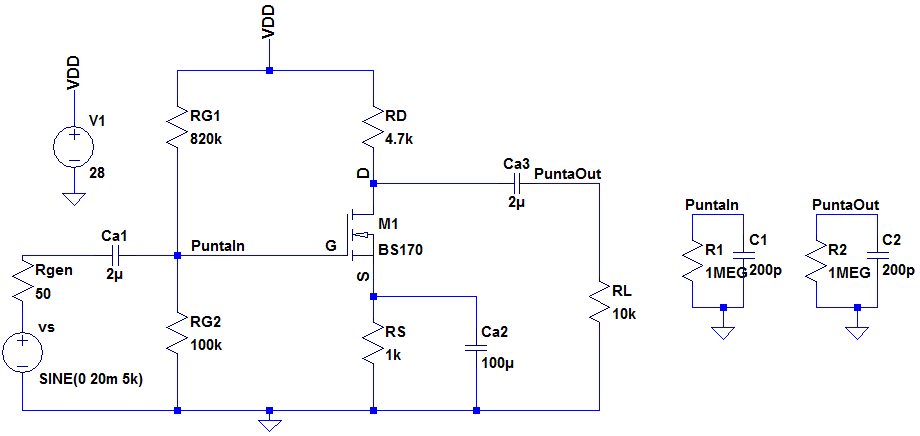
\includegraphics[scale=0.7]{circuitos/A_circuito_simu.png}
\caption{Circuito que se medirá, incluyendo puntas X1}
\label{fig:A_circuito_simu}
\end{figure}


En primer lugar se simuló en \emph{Spice} el punto de operación del circuito \ref{fig:A_circuito_simu} y se obtuvieron los valores de tabla \ref{table:tabla_Q_simu}:

\begin{table}[H]
    \centering
    \begin{tabular}{|c|c|c|c|} %aca pones la cantidad de columnas, te faltaba 1. la c indica que esta centrado el dato en su celda y las | son cada linea vertical de la tabla
    \hline
    $I_D$ & $V_{G}$ & $V_{S}$ & $V_{D}$ \\ \hline
     $1.09\,\unit{mA}$ & $3.04\,\unit{V}$  & $1.09\,\unit{V}$  & $22.9\,\unit{\ V}$  \\ \hline
    \end{tabular}
    \caption{Valores de tensiones contra común y corriente simulados}
    \label{table:tabla_Q_simu}
    \end{table}

Estos valores difieren de los obtenidos teóricamente (ver tabla
\ref{table:tabla_Q}), debido a que para el cálculo teórico se usó el
valor típico de la tensión umbral que no coincide con el que usa el
modelo de \emph{Spice}. 

\subsubsection{Dispersión del punto Q}
Modificando el K y la tensión umbral del archivo
\texttt{BS170.sub} se obtienen los valores de la tabla \ref{table:tabla_dispQ_simu}, puede verse que se obtuvieron valores muy cercanos a los de la tabla \ref{table:tabla_dispQ}.

\begin{table}[H]
\centering
\begin{tabular}{|c|c|c|c|} %aca pones la cantidad de columnas, te faltaba 1. la c indica que esta centrado el dato en su celda y las | son cada linea vertical de la tabla
\hline
Parámetro & $V_{T}=1.47\,\unit{V}$ y $K=160\,\unit{\frac{mA}{V^2}}$ &  $V_{T}=1.824\,\unit{V}$ y $K=123.3\,\unit{\frac{mA}{V^2}}$ & $V_{T}=2.73\,\unit{V}$ y $K=86\,\unit{\frac{mA}{V^2}}$  \\ \hline
$I_D$ & $1.43\,\unit{mA}$  &  $1.09\,\unit{mA}$ & $0.2\,\unit{mA}$   \\ \hline
$V_{DS}$ & $19.81\,\unit{V}$ & $21.81\,\unit{V}$  &  $26.64\,\unit{V}$  \\ \hline
$V_{GS}$ & $1.61\,\unit{V}$ & $1.95\,\unit{V}$ & $2.80\,\unit{V}$  \\ \hline
\end{tabular}
\caption{Tabla comparativa de los puntos Q con la dispersión de los parámetros simulados }
\label{table:tabla_dispQ_simu}
\end{table}

\subsubsection{Ganancia}
Para el calculo de $A_v$ se realizo un análisis en AC del circuito \ref{fig:A_circuito_simu} y luego se gráfico la tensión de salida dividido la tensión de entrada obteniéndose el gráfico \ref{fig:A_acAv}

\begin{figure}[H]
\centering
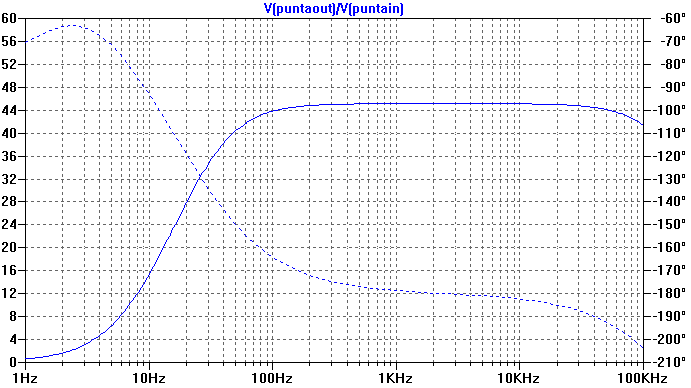
\includegraphics[scale=0.7]{simulaciones/A_acAv.png}
\caption{Ganancia $A_v$ en función de la frecuencia}
\label{fig:A_acAv}
\end{figure}

Del gráfico \ref{fig:A_acAv}, se decide medir a $1\,\unit{kHz}$, ya que se tiene una ganancia de aproximadamente $-45$, valor muy próximo al deseado. 

\subsubsection{Dispersión de la ganancia}
Luego, se modificó el modelo de \emph{Spice} nuevamente para obtener como varia la ganancia con la dispersión de Q para $1\,\unit{kHz}$ (ver figuras \ref{fig:A_acAvmax} y \ref{fig:A_acAvmin}). En la tabla \ref{table:tabla_AvQ_simu} puede verse como varia la ganancia con los parámetros. Cabe destacar que para el caso de $V_{T}=2.73\,\unit{V}$ y $K=86\,\unit{\frac{mA}{V^2}}$ la ganancia varia mucho respecto al calculo teórico debido a que, al simular, la tensión $V_{GS}$ queda muy próxima a la tensión $V_{T}$ y \emph{Spice} cambia el modelo con el que trabaja.

\begin{figure}[H]
\centering
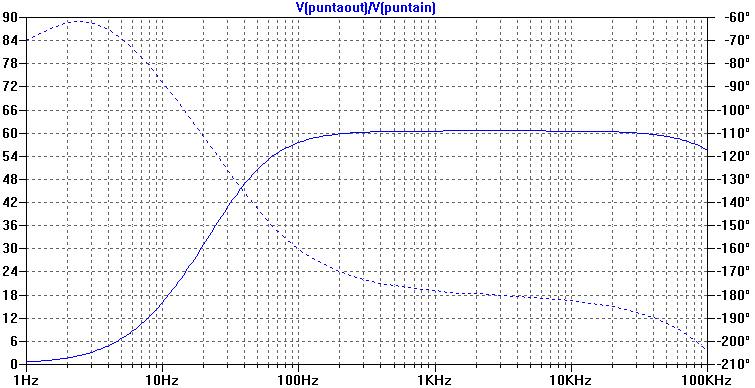
\includegraphics[scale=0.7]{simulaciones/A_acAvmax.png}
\caption{Ganancia $A_v$ en función de la frecuencia con $V_{T}=1.47\,\unit{V}$ y $K=160\,\unit{\frac{mA}{V^2}}$ }
\label{fig:A_acAvmax}
\end{figure}

\begin{figure}[H]
\centering
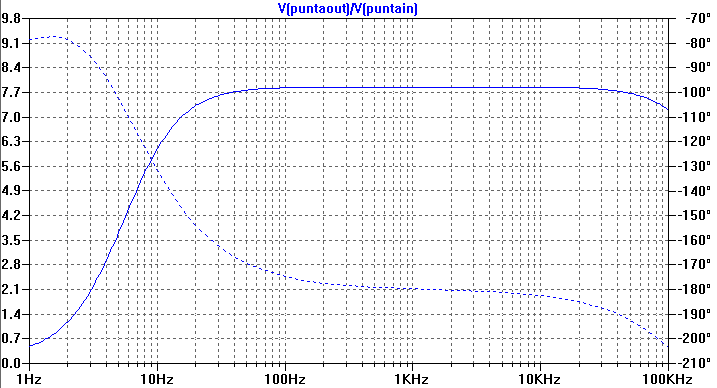
\includegraphics[scale=0.7]{simulaciones/A_acAvmin.png}
\caption{Ganancia $A_v$ en función de la frecuencia con $V_{T}=2.73\,\unit{V}$ y $K=86\,\unit{\frac{mA}{V^2}}$}
\label{fig:A_acAvmin}
\end{figure}

\begin{table}[H]
\centering
\begin{tabular}{|c|c|c|c|} %aca pones la cantidad de columnas, te faltaba 1. la c indica que esta centrado el dato en su celda y las | son cada linea vertical de la tabla
\hline
Parámetro & $V_{T}=1.47\,\unit{V}$ y $K=160\,\unit{\frac{mA}{V^2}}$ & $V_{T}=1.824\,\unit{V}$ y $K=123.3\,\unit{\frac{mA}{V^2}}$ & $V_{T}=2.73\,\unit{V}$ y $K=86\,\unit{\frac{mA}{V^2}}$  \\ \hline
$A_v$ & -61 & -45 & -8   \\ \hline
\end{tabular}
\caption{Tabla comparativa de las ganancias con respecto a la variación del punto Q simuladas a $1\,\unit{kHz}$  }
\label{table:tabla_AvQ_simu}
\end{table}

\subsubsection{Resistencia de entrada}
Del análisis en AC del circuito \ref{fig:A_simuRi}, se gráfico la tensión de entrada divido la corriente de entrada para calcular la resistencia de entrada

\begin{figure}[H]
\centering
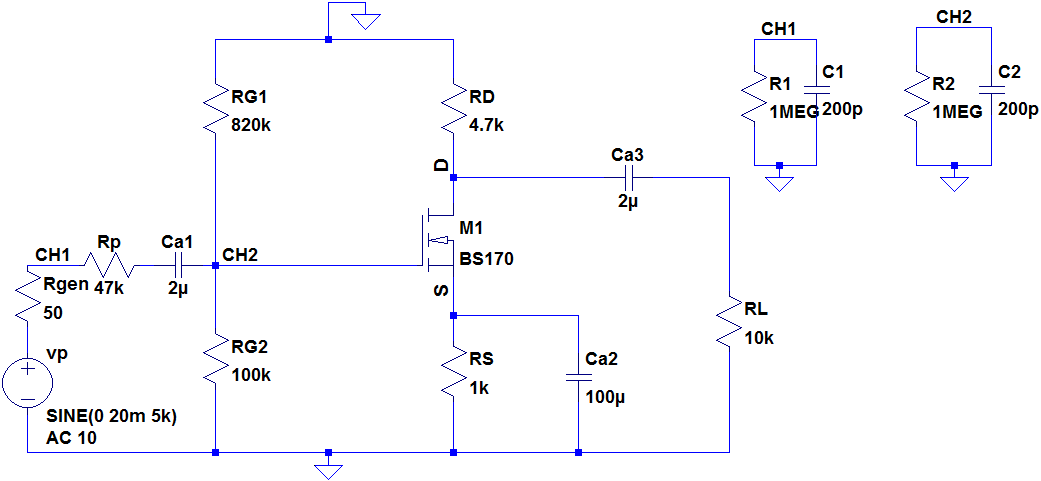
\includegraphics[scale=0.6]{circuitos/A_simuRi.png}
\caption{Circuito para simular y medir la resistencia de entrada $R_i$}
\label{fig:A_simuRi}
\end{figure}


\begin{figure}[H]
\centering
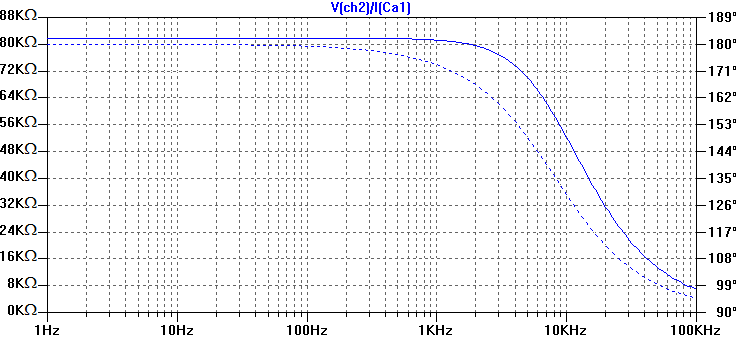
\includegraphics[scale=0.7]{simulaciones/A_acRi.png}  % trata de que no queden tan pegados al margen, fijate que al costadito tenias un warning
\caption{Resistencia de entrada $R_i$ en función de la frecuencia}
\label{fig:A_acRi}
\end{figure}

Puede observarse de la figura \ref{fig:A_acRi} que para $1\,\unit{kHz}$, la resistencia de entrada sigue siendo mayor a $10\,\unit{k\Omega}$

\subsubsection{Resistencia de salida}
Para simular $R_o$ en AC se utilizó el circuito \ref{fig:A_simuRo}, donde graficando la tensión $CH2$ dividido la corriente por el capacitor $C_{a3}$ se obtiene el gráfico \ref{fig:A_acRo}:

\begin{figure}[H]
\centering
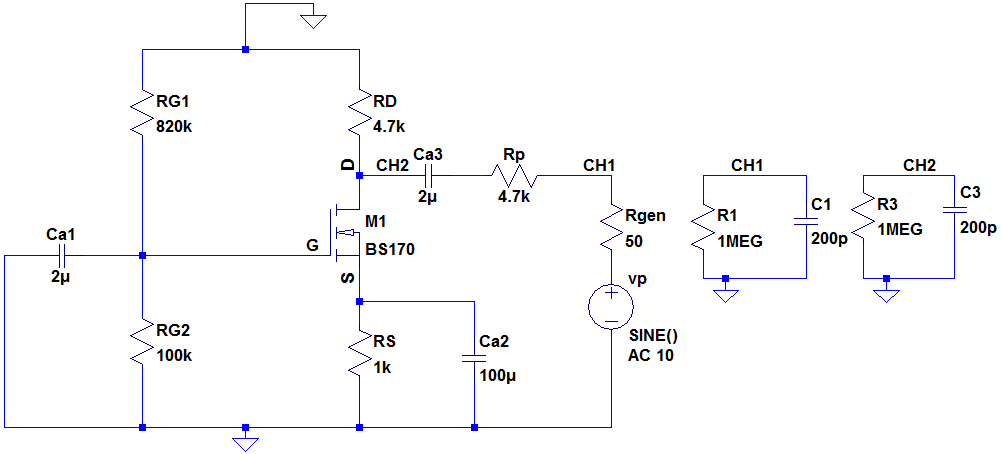
\includegraphics[scale=0.6]{circuitos/A_simuRo.png}
\caption{Circuito para simular y medir la resistencia de salida $R_o$}
\label{fig:A_simuRo}
\end{figure}

\begin{figure}[H]
\centering
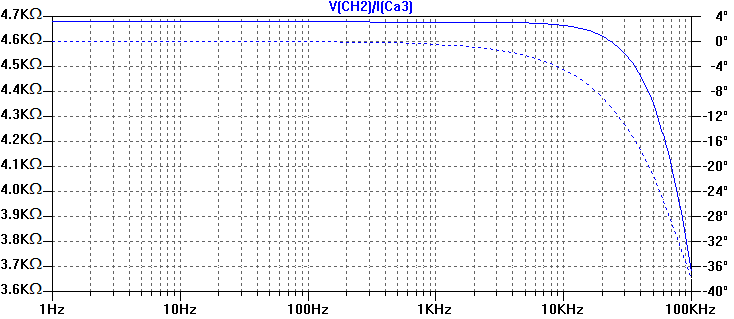
\includegraphics[scale=0.75]{simulaciones/A_acRo.png}
\caption{Resistencia de salida $R_o$ en función de la frecuencia}
\label{fig:A_acRo}
\end{figure}


\subsubsection{Rango de frecuencias valido}
De la figura \ref{fig:A_acAv} puede observarse que se tiene el valor deseado de $A_v$ entre $100\,\unit{Hz}$ y $100\,\unit{kHz}$. Para este rango de frecuencias la ganancia es aproximadamente de $-45$,. Por otro lado, observando la figura \ref{fig:A_acRi}, puede verse que en el mismo rango de frecuencias de antes se obtiene el valor de $R_i$ deseado, que si bien varia, se mantiene siempre mayor a $10\,\unit{k\Omega}$. Cabe destacar que en el rango de frecuencias donde se obtiene la resistencia de entrada y ganancia deseada la resistencia de salida presenta variaciones que no se tomaron en cuenta debido a que el diseño no presentaba requerimientos para este parámetro. Para todas las mediciones se utilizó punta x1 ya que se quiere saber el comportamiento de la ganancia y la resistencia de entrada en frecuencias cercanas a $1\,\unit{kHz}$, que es donde se realizaran las mediciones (debido a que a esta frecuencia se logran las especificaciones requeridas).

\subsubsection{Máxima excursión de salida}
Debido a que la máxima excursión de salida es de $2.23\,\unit{V}$, utilizando que $A_v=A_{vs}=-43.5$ (Debido a que la resistencia de entrada es mucho mayor a la resistencia del generador), se obtiene que la máxima señal del generador de entrada es aproximadamente $51\,\unit{mV}$. Usando esta tensión, como tensión del generador de entrada, se observa  en la figura \ref{fig:A_trans} que la señal de salida se deforma, pero no recorta.

\begin{figure}[H]
\centering
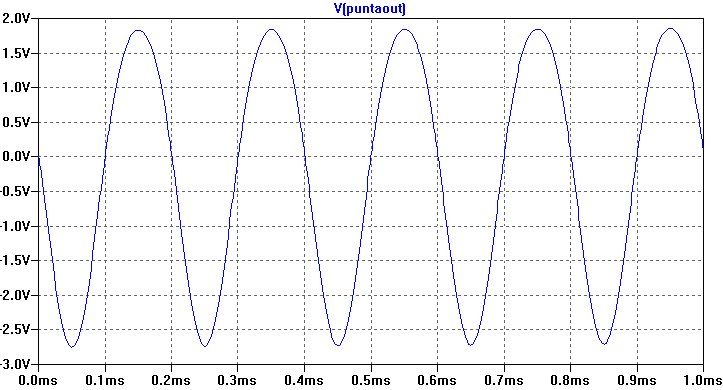
\includegraphics[scale=0.7]{simulaciones/A_trans.png}
\caption{Señal de salida cuando la entrada es $51\,\unit{mV}$ }
\label{fig:A_trans}
\end{figure}

Si bien la señal presenta deformación, el resultado obtenido es valido. Esto se debe a que, como se analizó de la ecuación \ref{eq:A_max_ent}, para valores de $v_{gs}$ menores a $55\,\unit{mV}$, sigue valiendo la linealidad del modelo, por lo que para tensiones de entrada que no superen este valor, es valido pensar al dispositivo como lineal. En la figura \ref{fig:A_trans15} , se usó como tensión del generador $15\,\unit{mV}$, y puede observarse que la señal mejora su forma, es decir, se obtiene una señal senoidal. 

\subsubsection{Valores de los parámetros obtenidos}
En la tabla \ref{table:param_simu} pueden verse los parametros obtenidos mediante simulación.



\begin{figure}[H]
\centering
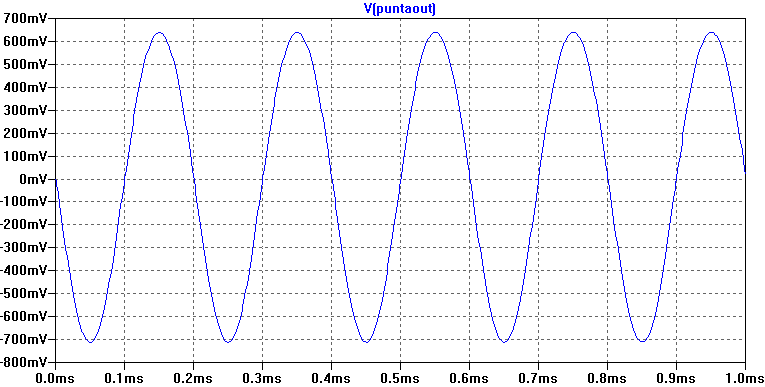
\includegraphics[scale=0.7]{simulaciones/A_trans15.png}
\caption{Señal de salida cuando la entrada es $15\,\unit{mV}$ }
\label{fig:A_trans15}
\end{figure}

\begin{table}[H]
    \centering
    \begin{tabular}{|c|c|c|} %aca pones la cantidad de columnas, te faltaba 1. la c indica que esta centrado el dato en su celda y las | son cada linea vertical de la tabla
    \hline
    $A_v$ & $R_i$  & $R_o$ \\ \hline
     -45 & $80\,\unit{k\Omega}$  & $4.5\,\unit{k\Omega}$   \\ \hline
    \end{tabular}
    \caption{Tabla con los parametros calculados mediante simulación a $1\,\unit{k\ Hz}$ utilizando los parametros por defecto de Spice para el transistor}
    \label{table:param_simu}
    \end{table}



\subsection{Mediciones}

\subsubsection{Polarización del transistor}
En primer lugar, se midieron las tensiones contra común y la corriente en el punto de operación, utilizando el circuito de la figura \ref{fig:A_circuito_simu} y un multimetro (DT830B de la marca UNI-T), con el generador de entrada apagado. Los valores obtenidos se detallan en la tabla \ref{table:tabla_Q_medido}.

\begin{table}[H]
    \centering
    \begin{tabular}{|c|c|c|c|} %aca pones la cantidad de columnas, te faltaba 1. la c indica que esta centrado el dato en su celda y las | son cada linea vertical de la tabla
    \hline
    $I_D$ & $V_{G}$ & $V_{S}$ & $V_{D}$ \\ \hline
     $1.59\,\unit{mA}$ & $2.68\,\unit{\ V}$  & $1.59\,\unit{\ V}$  & $20.7\,\unit{\ V}$  \\ \hline
    \end{tabular}
    \caption{Valores de tensiones contra comun y corriente medidos}
    \label{table:tabla_Q_medido}
    \end{table}

\subsubsection{Ganancia}
Luego se midió $A_v$, utilizando nuevamente el circuito \ref{fig:A_circuito_simu}, pero con el generador de tensión $v_s$ en $28\,\unit{mV}$ y aproximadamente frecuencia de $1\,\unit{KHz}$. Este valor de tensión fue elegido para evitar distorsión y para poder seguir suponiendo que el transistor se comporta linealmente (ver ecuación \ref{eq:A_max_ent}). La frecuencia fue elegida debido a que en ese valor, como se había analizado previamente, se obtienen los valores deseados de ganancia y resistencia de entrada. De la medición se obtuvo el gráfico de la figura \ref{fig:1_Av}. De este gráfico, utilizando la ecuación \ref{eq:A_Av} (Debido a que $R_i$ es mucho mas grande que $R_s$, $A_v$ y $A_{vs}$ son aproximadamente iguales), se obtiene que la ganancia vale aproximadamente $A_v=-20$. Este valor se aleja del deseado, pero el circuito aun sigue amplificando la señal de entrada.


\begin{figure}[H]
\centering
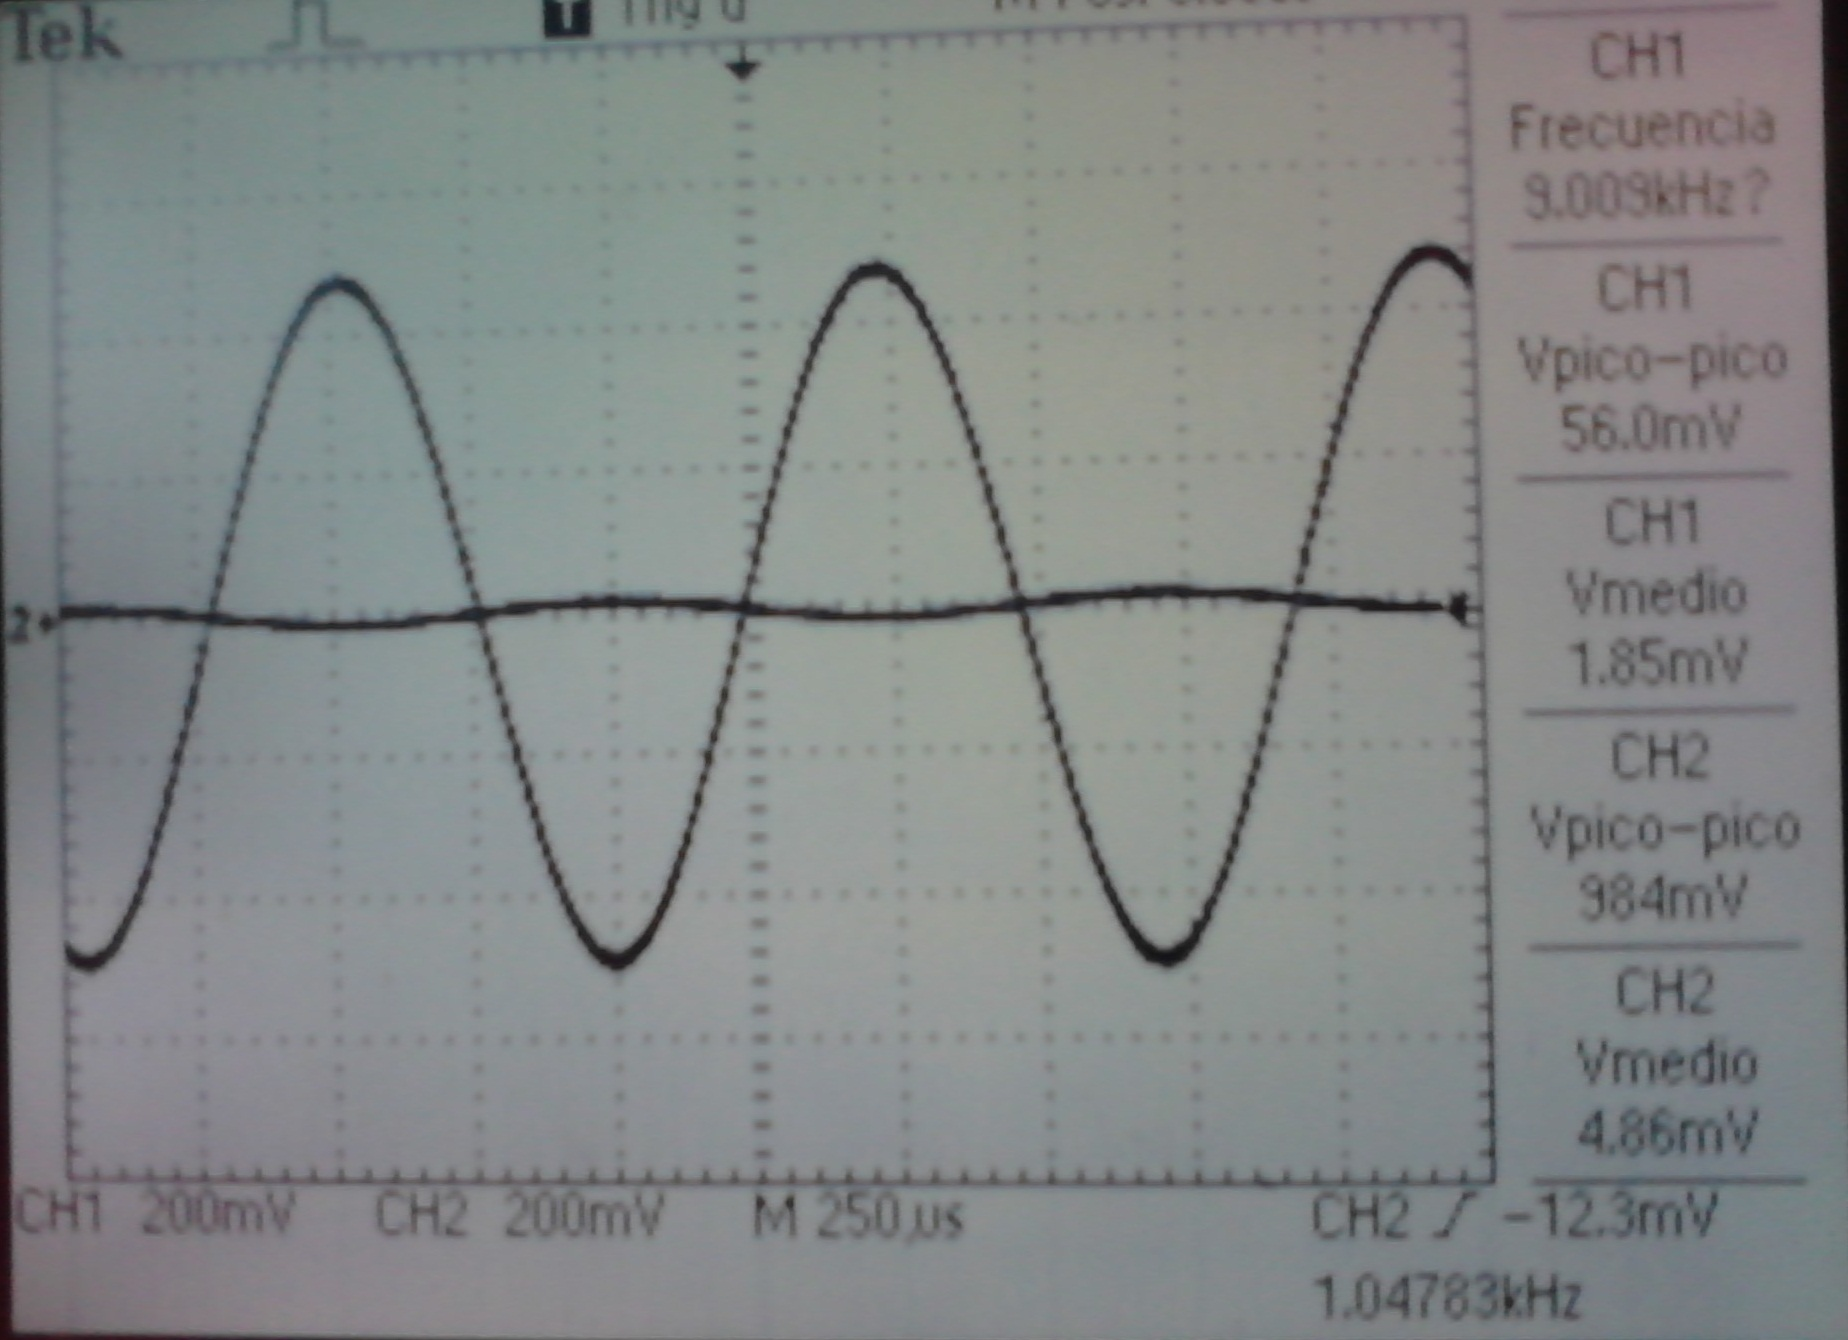
\includegraphics[scale=0.2]{mediciones/1_Av.jpg}
\caption{Señal de salida (CH2) y señal de entrada (CH1)}
\label{fig:1_Av}
\end{figure}

\subsubsection{Validez del modelo lineal}
A continuación, se aumentó la tensión del generador a $80\,\unit{mV}$ para analizar la salida cuando el transistor deja de comportarse linealmente según el criterio optado. El gráfico de esta medición puede observarse en la figura \ref{fig:1_Av_def}. Del mismo puede verse que la salida se deforma, es decir, no se obtiene a la salida una senoidal perfecta, tal como se había predicho.


\begin{figure}[H]
\centering
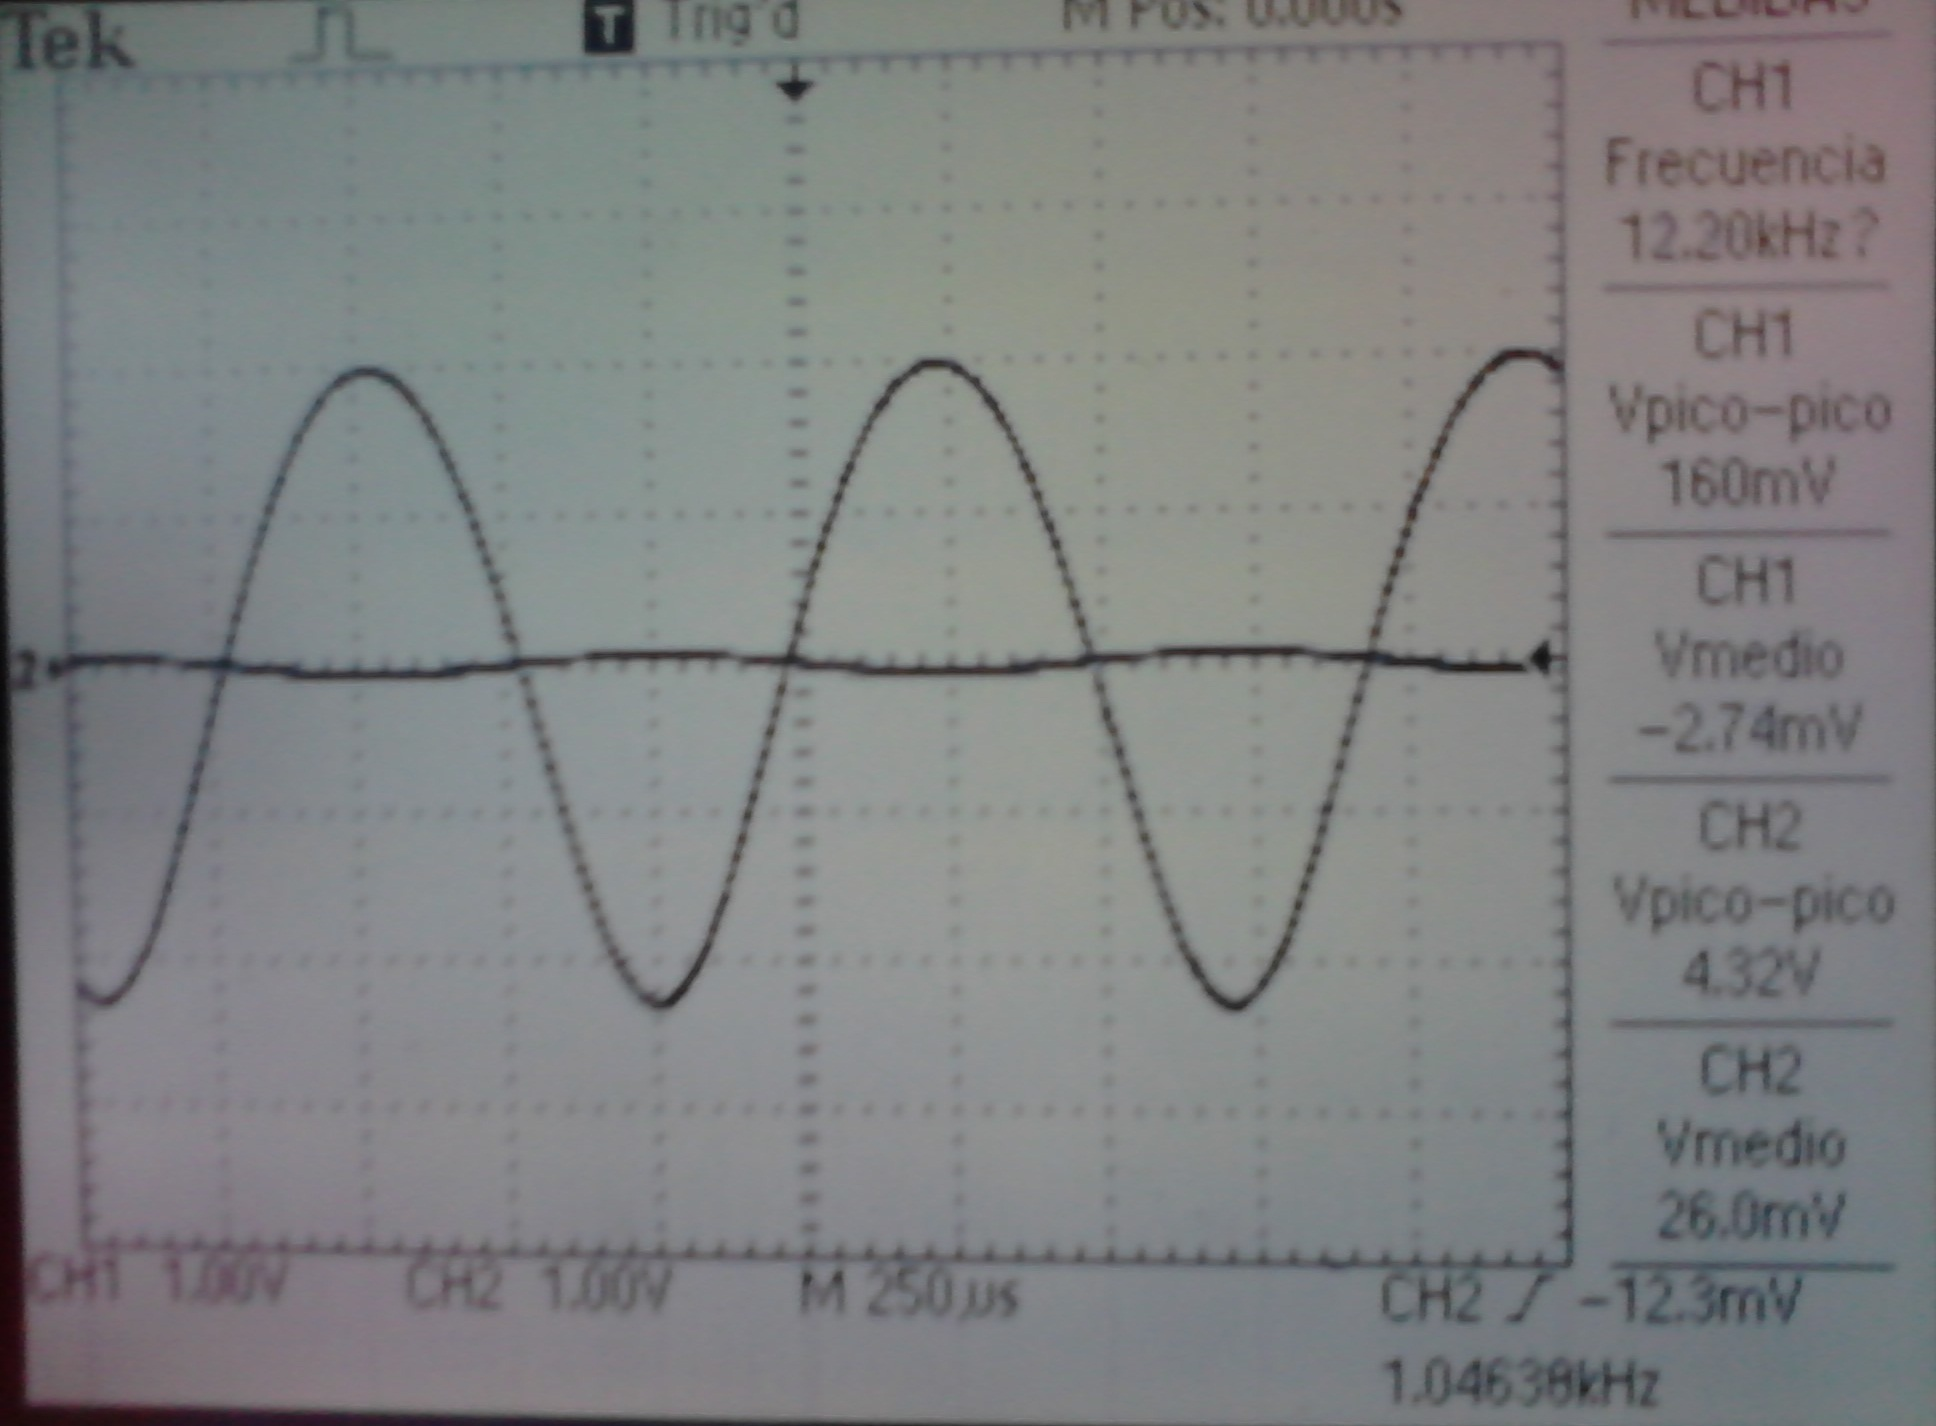
\includegraphics[scale=0.19]{mediciones/1_Avdef.jpg}
\caption{Señal de salida (CH2) y señal de entrada (CH1)}
\label{fig:1_Av_def}
\end{figure}

\subsubsection{Resistencia de entrada}
Para medir la resistencia de entrada, se utilizó el circuito de la figura \ref{fig:A_simuRi}. Se eligió utilizar una tensión del generador de $362\,\unit{mV}$ y frecuencia de $1\,\unit{kHz}$ porque es la frecuencia a la que se obtienen los valores deseados de ganancia y resistencia de entrada. La resistencia en serie al generador fue elegida de $47\,\unit{k\Omega}$, ya que del cálculo teórico se espera tener aproximadamente $80\,\unit{k\Omega}$ de resistencia de entrada. De la medición, se obtuvieron en el osciloscopio las señales vistas en la figura \ref{fig:1_Ri}


\begin{figure}[H]
\centering
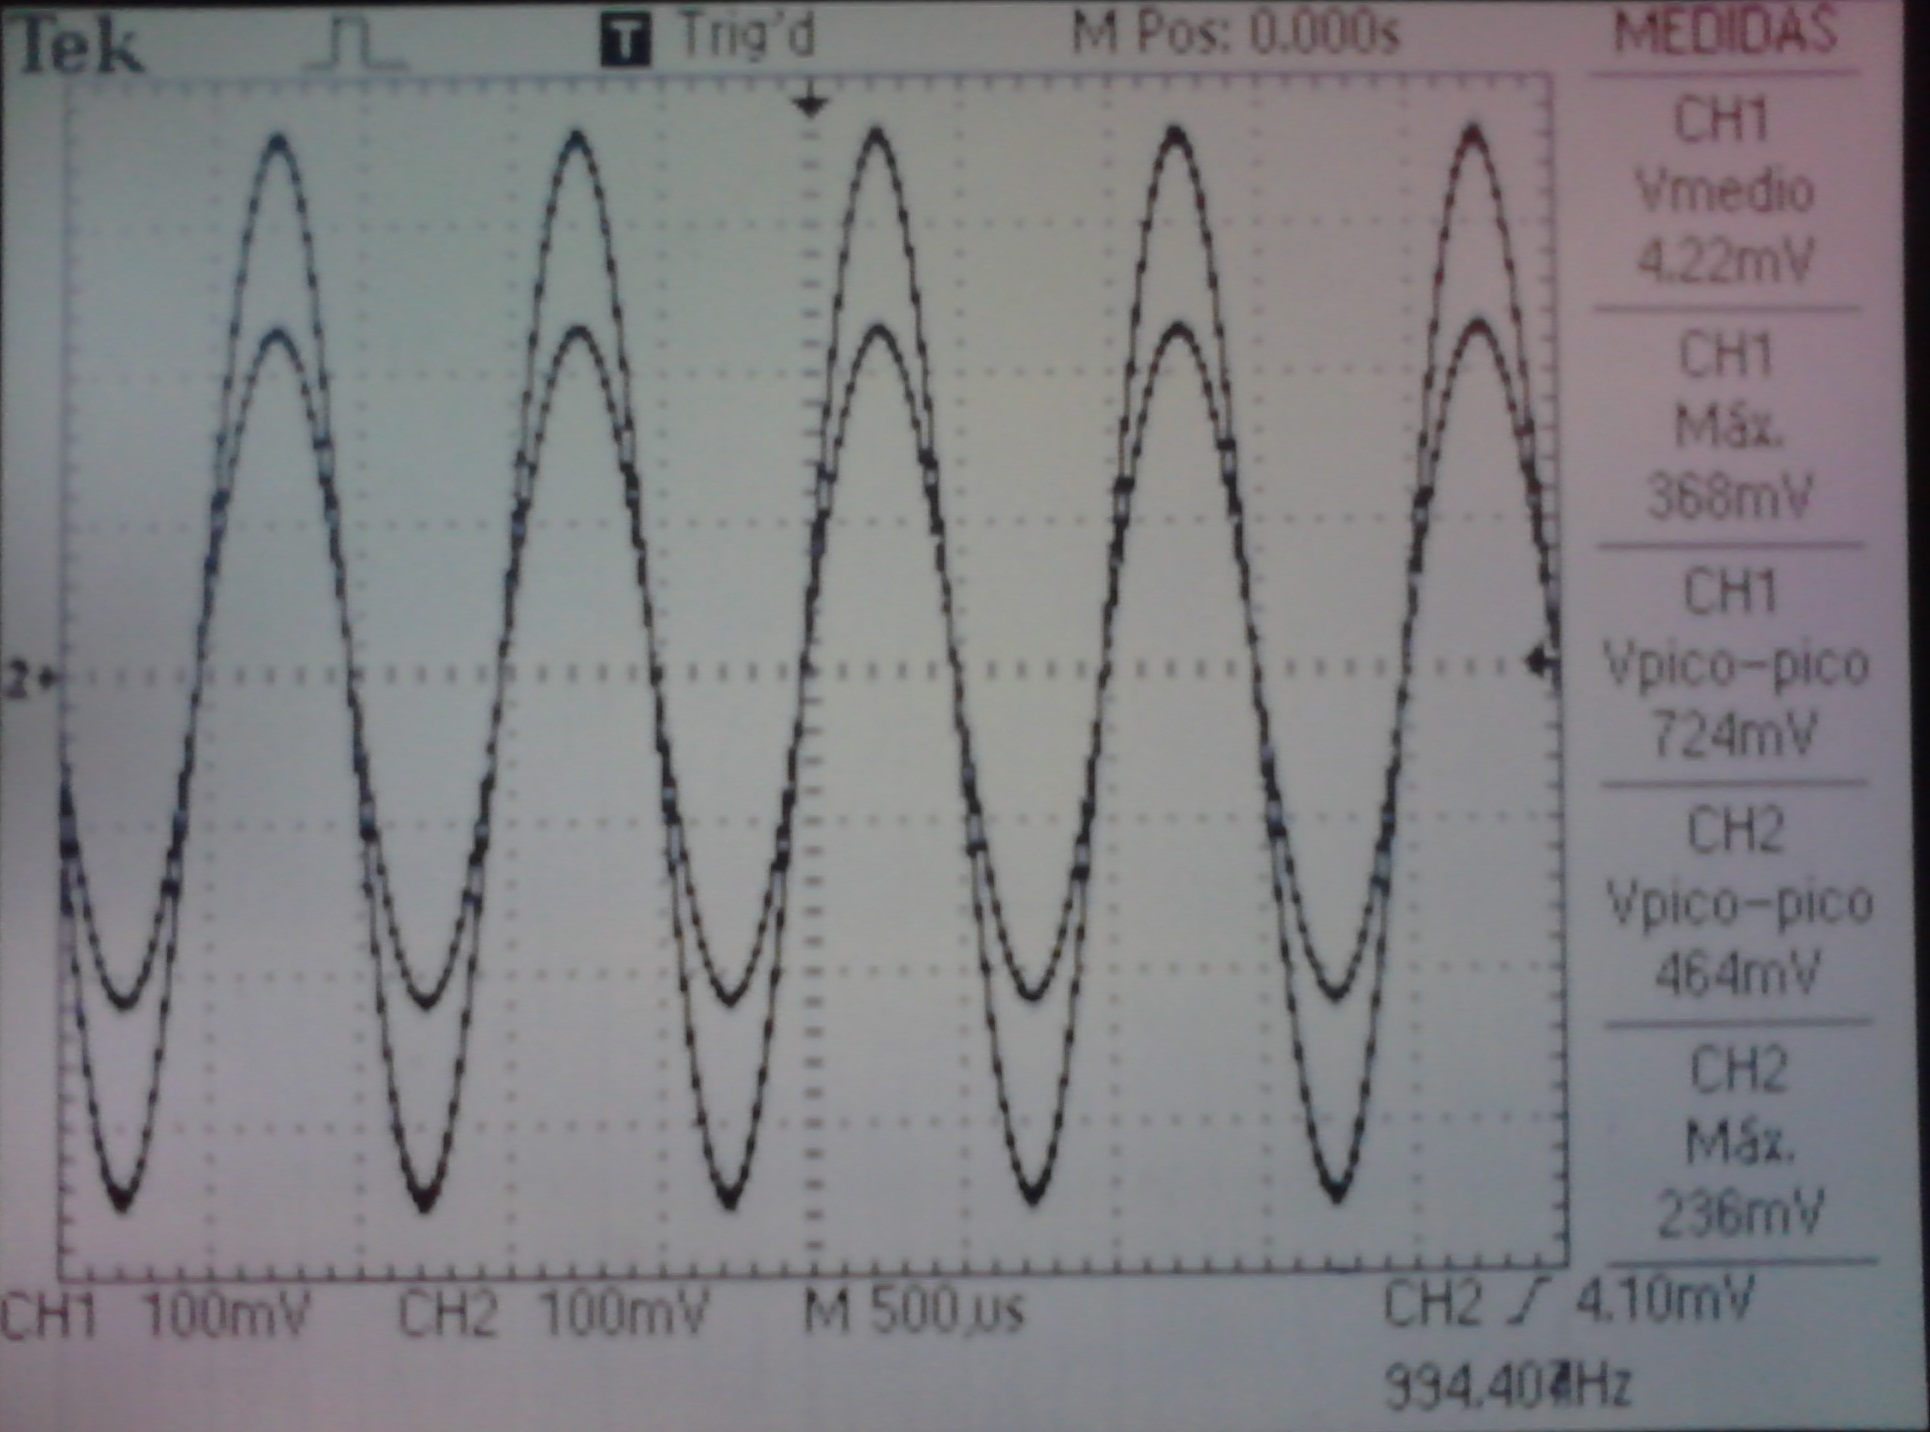
\includegraphics[scale=0.2]{mediciones/1_Ri.jpg}
\caption{Señales de los canales 1 y 2 para calcular la resistencia de entrada}
\label{fig:1_Ri}
\end{figure}

Para calcular la resistencia $R_i$ se realizan los siguientes cálculos observando los valores máximos de las tensiones de la figura \ref{fig:1_Ri} y el circuito \ref{fig:A_simuRi}.

\begin{equation}
    v_{R_3}=v_{CH1}-v_{CH2}
    \label{fig:ec1}
\end{equation}

\begin{equation}
    i_{R_p}=\frac{v_{R_p}}{Rp}
    \label{fig:ec2}
\end{equation}

Finalmente la resistencia de entrada se obtiene como 

\begin{equation}
    R_{i}=\frac{v_{R_p}}{i_{R_p}}
    \label{fig:ec3}
\end{equation}

Por lo tanto se obtiene una resistencia de entrada de aproximadamente $84\,\unit{k\Omega}$

\subsubsection{Resistencia de salida}
Para medir la resistencia de salida, se utilizó el circuito de la figura \ref{fig:A_simuRo} . Se eligió utilizar una tensión del generador de $360\,\unit{mV}$ y frecuencia de $1\,\unit{kHz}$ porque es la frecuencia a la que se logran tener las especificaciones deseadas. La resistencia en serie al generador se eligió de $4.7\,\unit{k\Omega}$ ya que del cálculo teórico se espera tener una resistencia de salida del mismo valor. De la medición, se obtuvieron en el osciloscopio las señales vistas en la figura \ref{fig:1_Ro}.


\begin{figure}[H]
\centering
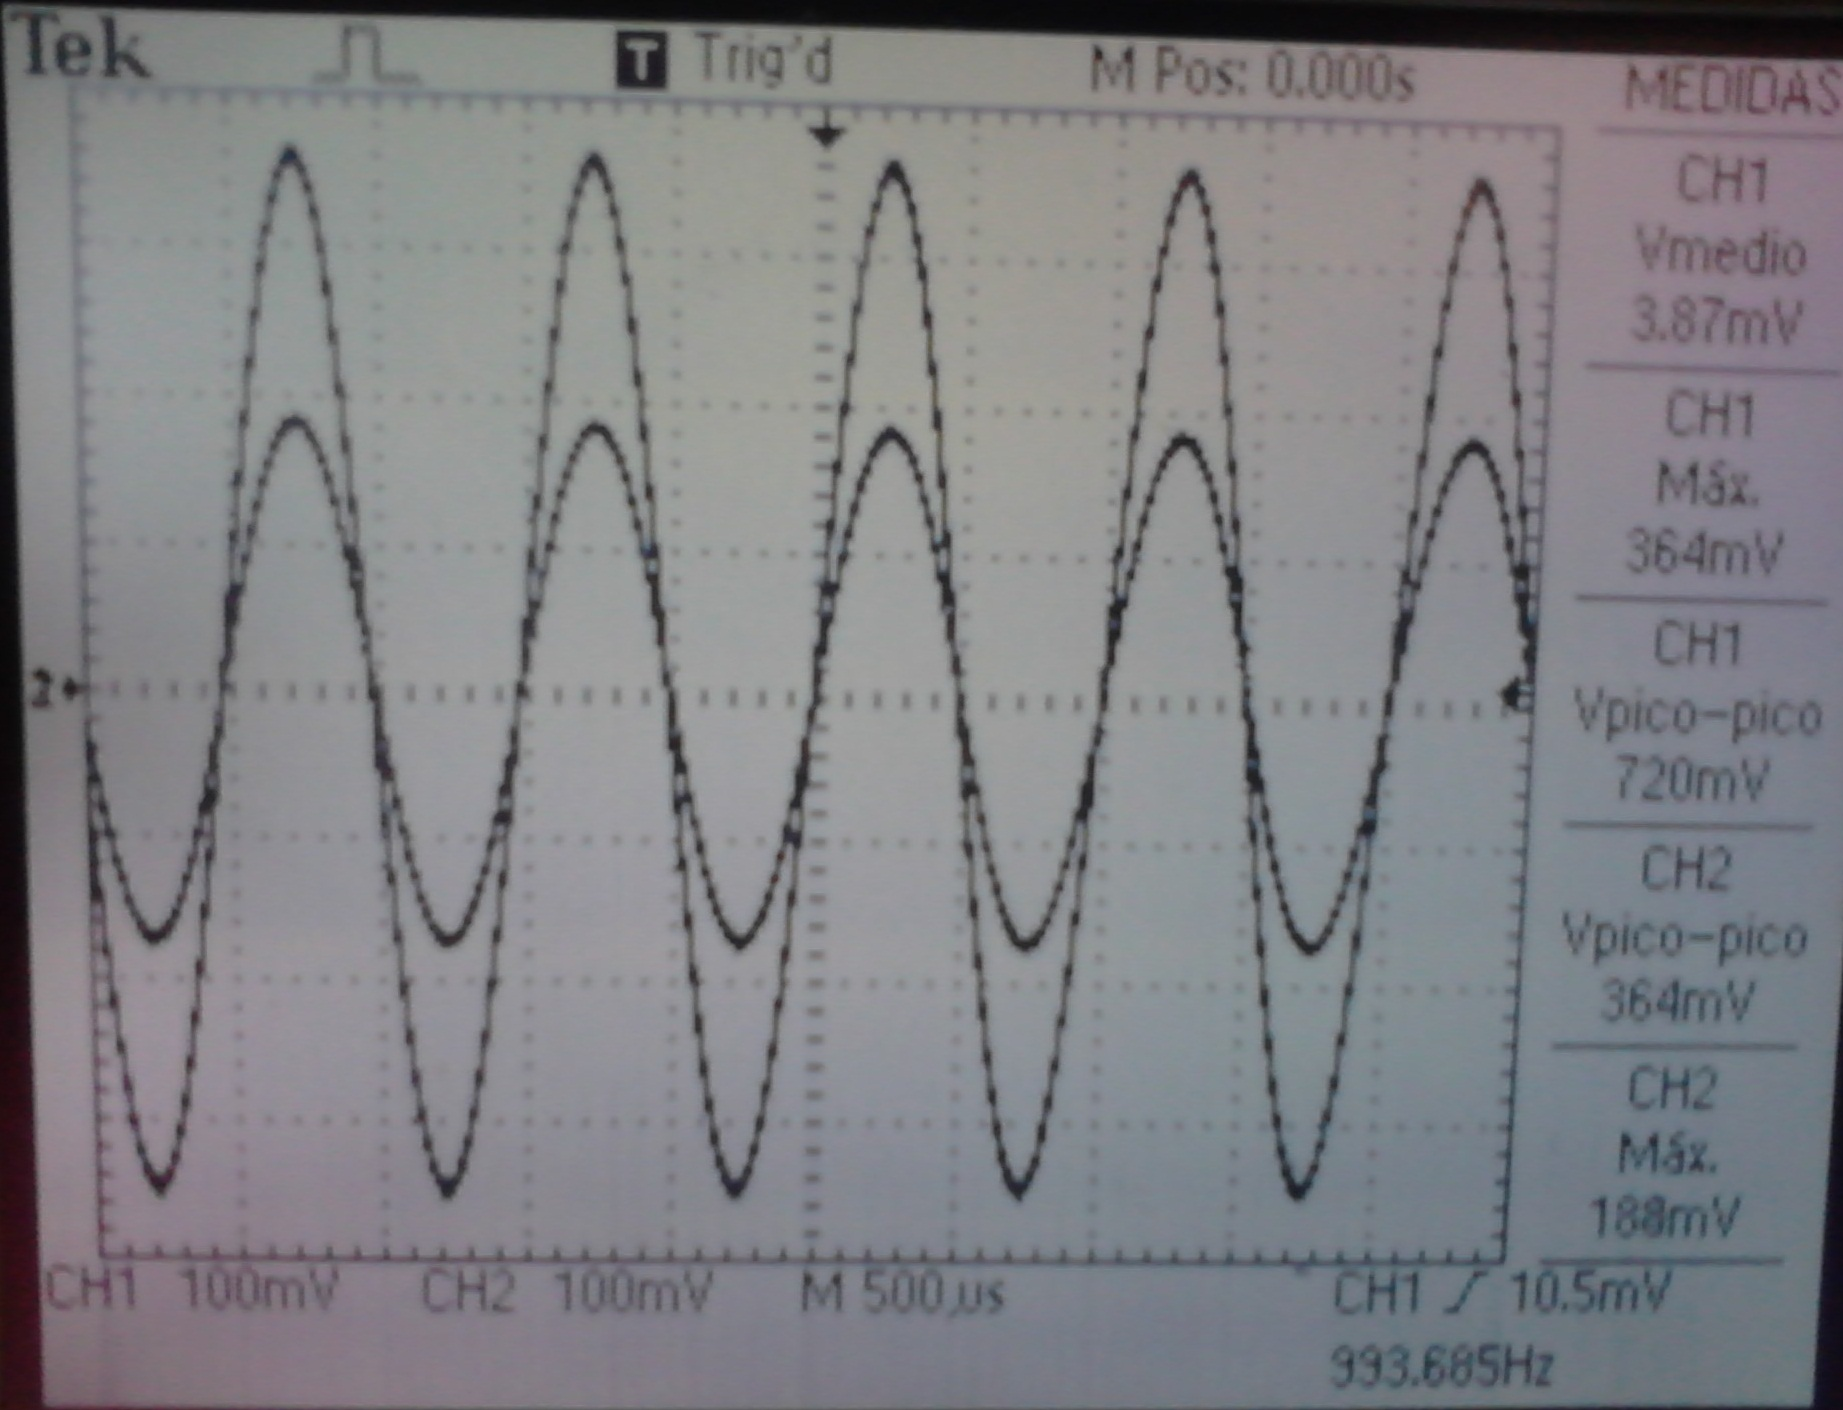
\includegraphics[scale=0.2]{mediciones/1_Ro.jpg}
\caption{Señales de los canales 1 y 2 para calcular la resistencia de salida}
\label{fig:1_Ro}
\end{figure}

Utilizando las tensiones máximas de la figura \ref{fig:1_Ro} y el circuito \ref{fig:A_simuRo}, junto con las ecuaciones \ref{fig:ec1}, \ref{fig:ec2} y \ref{fig:ec3}, se obtiene que la resistencia de salida es de aproximadamente $5\,\unit{k\Omega}$. 

\subsubsection{Valores de los parámetros obtenidos}
En la tabla  \ref{table:param_med} pueden observarse los parámetros del amplificador medidos.

\begin{table}[H]
    \centering
    \begin{tabular}{|c|c|c|} %aca pones la cantidad de columnas, te faltaba 1. la c indica que esta centrado el dato en su celda y las | son cada linea vertical de la tabla
    \hline
    $A_v$ & $R_i$  & $R_o$ \\ \hline
     -20 & $84\,\unit{k\Omega}$  & $5\,\unit{k\Omega}$   \\ \hline
    \end{tabular}
    \caption{Tabla con los parametros medidos a $1\,\unit{k\ Hz}$}
    \label{table:param_med}
    \end{table}

\subsection{Resultados}

En la tabla  \ref{table:puntoq_comp} pueden verse las tensiones y corrientes en el
punto Q obtenidas a traves del calculo teórico, simulación y medición, y en la tabla
\ref{table:puntoq_comperror} los errores del calculo teórico y la simulación respecto
a la medición. Puede verse que el error mas grande se tiene en la corriente, esto
puede deberse a que el parámetro $V_{T}$ según la hoja de datos, puede variar desde
$0.8\,\unit{V}$ hasta $3\,\unit{V}$, es decir, presenta una dispersión mayor al 30\%
del valor típico como se tuvo en cuenta tanto en los cálculos teóricos como en la
simulación. Por otro lado, el valor de parámetro $k$ es difícil de determinar, y, al
igual que para el parámetro $V_{T}$, también se analizó solamente una dispersión del
30\% del mismo a partir del valor típico. Por lo tanto, debido a que el rango de los
parámetros propios del transistor en el que se analizo la operación del mismo es menor al rango
real, pueden tenerse errores como los encontrados. En la tabla
\ref{table:puntoq_comp} pueden verse los valores de ganancia, resistencia de entrada
y salida obtenidos a partir de la medición, simulación y cálculo teórico, y en la
tabla \ref{table:puntoq_comperror} los errores de los valores obtenido mediante
cálculo teórico y simulación respecto a la medición. De las expresiones
\ref{eq:A_Av}, \ref{eq:A_gm}, \ref{eq:A_Rig}, \ref{eq:A_Ri}, \ref{eq:A_Rod},
\ref{eq:A_Ro}, puede observarse que las resistencias de entrada y de salida, pueden
aproximarse a ser independientes del punto de polarización (en el entorno de valores de corrientes y tensiones en los que trabaja el transistor en este amplificador), por lo que se llega a que el error respecto a
la medición es chico por ambos métodos. Por otro lado la ganancia es dependiente de
la transconductancia, la cual depende de las tensiones $V_{T}$, $V_{GS}$, y de $k$, por lo que
por los mismos motivos analizados para el punto de polarización es lógico que
presente el mayor error.


    \begin{table}[H]
    \centering
    \begin{tabular}{|c|c|c|c|} %aca pones la cantidad de columnas, te faltaba 1. la c indica que esta centrado el dato en su celda y las | son cada linea vertical de la tabla
    \hline
    Parámetro & Teórico &  Simulación & Medición \\ \hline
    $I_D$ & $0.78\,\unit{mA}$  &  $1.09\,\unit{mA}$ & $1.59\,\unit{mA}$   \\ \hline
    $V_{G}$ & $3.04\,\unit{V}$ & $3.04\,\unit{V}$  &  $2.68\,\unit{V}$  \\ \hline
    $V_{D}$ & $24.35\,\unit{V}$ & $22.9\,\unit{V}$  &  $20.7\,\unit{V}$  \\ \hline
    $V_{S}$ & $0.83\,\unit{V}$ & $1.09\,\unit{V}$  &  $1.59\,\unit{V}$  \\ \hline
    $V_{DS}$ & $23.52\,\unit{V}$ & $21.81\,\unit{V}$  &  $19.11\,\unit{V}$  \\ \hline
    $V_{GS}$ & $2.21\,\unit{V}$ & $1.95\,\unit{V}$ & $1.09\,\unit{V}$  \\ \hline
    \end{tabular}
    \caption{Tabla comparativa de los puntos Q obtenidos mediante diferentes métodos }
    \label{table:puntoq_comp}
    \end{table}

    \begin{table}[H]
    \centering
    \begin{tabular}{|c|c|c|} %aca pones la cantidad de columnas, te faltaba 1. la c indica que esta centrado el dato en su celda y las | son cada linea vertical de la tabla
    \hline
    Parámetro & Teórico &  Simulación  \\ \hline
    $I_D$ & -51\%  & -31\%  \\ \hline
    $V_{G}$ & 13\% & 13\% \\ \hline
    $V_{D}$ & 18\% & 11\%  \\ \hline
    $V_{S}$ & -48\% & -31\%  \\ \hline
    $V_{DS}$ & 23\% & 14\%  \\ \hline
    $V_{GS}$ & 103\% & 79\%  \\ \hline
    \end{tabular}
    \caption{Tabla con los errores respecto a la medición de las corrientes y tensiones calculadas teoricamente y simuladas }
    \label{table:puntoq_comperror}
    \end{table}



\begin{table}[H]
    \centering
    \begin{tabular}{|c|c|c|c|} %aca pones la cantidad de columnas, te faltaba 1. la c indica que esta centrado el dato en su celda y las | son cada linea vertical de la tabla
    \hline
    Método & $A_v$ & $R_i$  & $R_o$ \\ \hline
    Teórico & -43.5 & $89\,\unit{k\Omega}$  & $4.7\,\unit{k\Omega}$   \\ \hline
    Simulación & -45 & $80\,\unit{k\Omega}$  & $4.5\,\unit{k\Omega}$   \\ \hline
    Medición & -20 & $84\,\unit{k\Omega}$  & $5\,\unit{k\Omega}$   \\ \hline
    \end{tabular}
    \caption{Tabla con los parametros obtenidos a $1\,\unit{k\ Hz}$ mediante diferentes métodos}
    \label{table:param_comp}
    \end{table}


\begin{table}[H]
    \centering
    \begin{tabular}{|c|c|c|c|} %aca pones la cantidad de columnas, te faltaba 1. la c indica que esta centrado el dato en su celda y las | son cada linea vertical de la tabla
    \hline
    Método & $A_v$ & $R_i$  & $R_o$ \\ \hline
    Teórico & 117\% & 6\%  & -6\%  \\ \hline
    Simulación & 125\% & -5\%  & -10\%  \\ \hline
   
    \end{tabular}
    \caption{Tabla con los errores de los parametros obtenidos a $1\,\unit{k\ Hz}$ mediante simulación y calculo teórico respecto a la medición}
    \label{table:param_comperror}
    \end{table}

















































\subsection{Preguntas}

{\color{OliveGreen}
¿La etapa amplificadora diseñada está realimentada para la señal?}\\

No, ya que tiene un capacitor en paralelo al resistor  $R_S$. Que para 
la señal se comporta como un corto. Eliminando así el efecto del resistor $R_S$ para la señal.\\

{\color{OliveGreen}
Si no lo está¿Qué elemento debería eliminarse o agregarse en el circuito para que esté
realimentado para la señal?. En ese caso, ¿qué se muestrearía a la salida y qué se 
sumaría a la entrada?. De acuerdo con esto, ¿qué parámetro de transferencia del amplificador
es el que se querría estabilizar si la realimentación fuese negativa?. Demostrar mediante
un análisis de incrementos si la realimentación es negativa.}\\

Debería eliminarse el capacitor que está en paralelo a $R_S$.
En este caso en la salida ocurre un muestreo de corriente y en la entrada se sumaría tensión.
Ya que por la resistencia $R_S$ circula la corriente de salida, que genera una caída de tensión
sobre $R_S$ que afecta a la tensión de entrada.
Con este tipo de realimentación se estabiliza $G_m$.
Al aumentar la corriente de salida, aumenta la tensión sobre el resistor $R_S$. Lo que
origina una disminución en la tensión de polarización $V_GS$, y de esta forma disminuyendo
la corriente de salida. Este decremento se opone al incremento inicial, por lo que
la realimentación es negativa. Desde el punto de vista del circuito de señal, teniendo en cuenta la resistencia de realimentación en el source, $R_S$, un incremento positivo del generador de entrada, $v_s$, produciría un incremento positivo en la tensión de entrada del circuito $v_i$ y $R_S$, entonces la nueva $v_i$ se calcula como

\begin{equation}
    v_{i}=v_{s}-v_{R_s}
\end{equation}

por lo que la nueva tensión de entrada del circuito será menor a la inicial. De esto puede notarse que la realimentación es negativa.




\section{Característica y parámetros de los dispositivos}

\subsection{Circuito utilizado}

Se propone utilizar el circuito mostrado en la figura 
\ref{circuito:simulacion_jfet} para obtener las características de salida 
($I_D$,$V_{DS}$) con $V_{GS}$ como parámetro.


\begin{figure}[H]
\centering
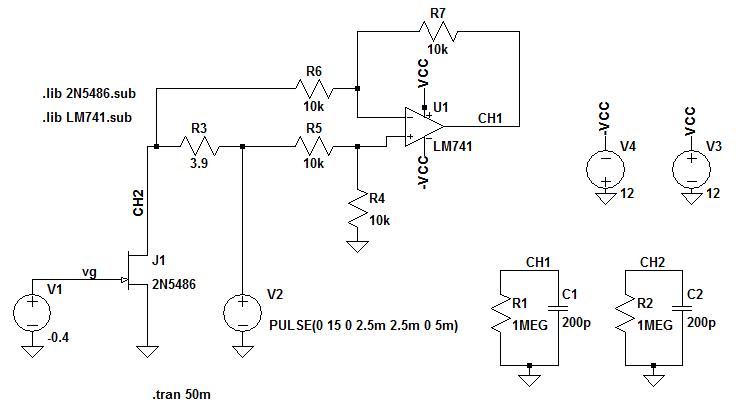
\includegraphics[scale=0.6]{circuitos/2_banco.png}
\caption{Circuito para la obtención de características de salida.}
\label{circuito:simulacion_jfet}
\end{figure}

Se utilizará el osciloscopio en modo XY y utilizando puntas directas.
Para obtener $V_{DS}$ se medirá con la punta del canal 2 en el terminal D del
transistor.
Para $I_D$ se medirá la tensión de salida del amplificador $V_{CH1}$ restador utilizando
la punta del canal 1.
Con las resistencias elegidas para el amplificador restador se obtendrá la diferencia
de tensión entre los terminales del resistor, para luego calcular la corriente
mediante la ecuación \ref{eq:I_D_jfet}. 

\begin{equation}
I_D = \frac{V_{CH1}}{R_3}
\label{eq:I_D_jfet}
\end{equation}


La fuente $V_2$ es una señal triangular de amplitud pico a pico de $10\,\unit{V}$ con
un offset de $5\,\unit{V}$. Con una frecuencia de $f=200\,\unit{Hz}$.

Luego se irá variando $V_{GS} = V_1$ directo desde la fuente para observar
distintas curvas.

\subsection{Simulación}

En las figuras \ref{fig:simulacion_jfet_0}, \ref{fig:simulacion_jfet_04},
\ref{fig:simulacion_jfet_1} y \ref{fig:simulacion_jfet_15} se muestran las curvas
obtenidas en \emph{Spice} para $V_{GS} = 0.0\,\unit{V}$, $V_{GS} = -0.4\,\unit{V}$,
$V_{GS} = -1.0\,\unit{V}$ y $V_{GS} = -1.5\,\unit{V}$ respectivamente.

Se obtiene de las curvas la corriente $I_D$ para $V_{DS} = 5\,\unit{V}$ para luego
poder ser comparadas con un modelo teórico simulado.

Se obtiene $I_D$ utilizando la ley de Ohm, mediante la ecuación \ref{eq:I_D_jfet}.

\[ \displaystyle I_D = \{\ 23.0\,\unit{mA} \ ;\ 31.0\,\unit{mA} \ ;\ 43.3\,\unit{mA} \ ;\ 51.3\,\unit{mA} \ \} \]

\begin{figure}[H]
\centering
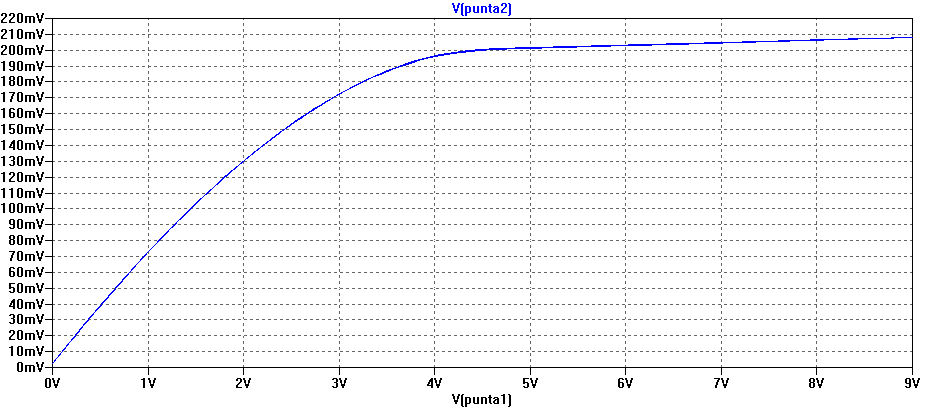
\includegraphics[scale=0.6]{simulaciones/2_vgs0_sim.png}
\caption{Curva obtenida con $V_{GS} = 0.0\,\unit{V}$.}
\label{fig:simulacion_jfet_0}
\end{figure}

\begin{figure}[H]
\centering
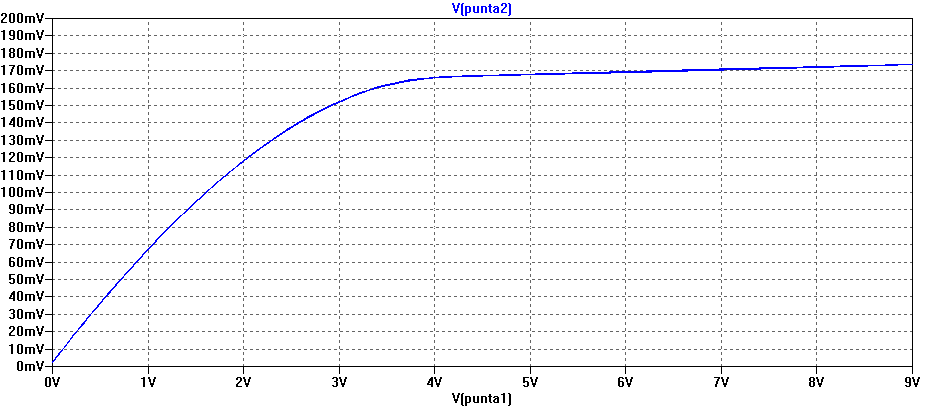
\includegraphics[scale=0.6]{simulaciones/2_vgs-04_sim.png}
\caption{Curva obtenida con $V_{GS} = -0.4\,\unit{V}$.}
\label{fig:simulacion_jfet_04}
\end{figure}

\begin{figure}[H]
\centering
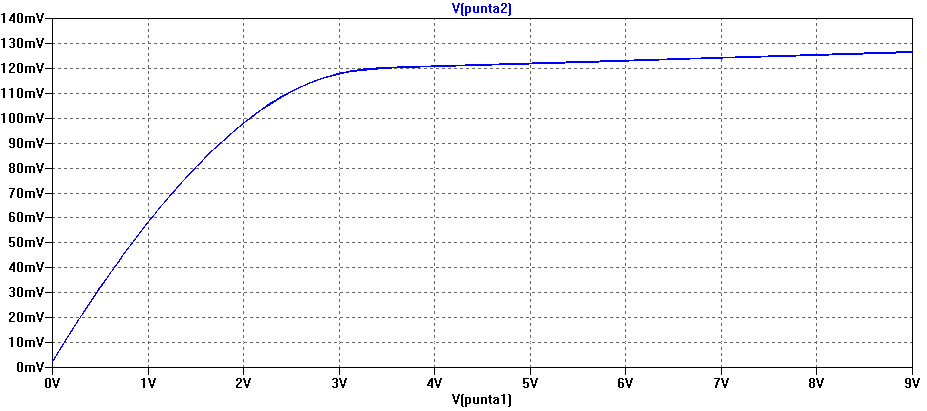
\includegraphics[scale=0.6]{simulaciones/2_vgs-1_sim.png}
\caption{Curva obtenida con $V_{GS} = -1.0\,\unit{V}$.}
\label{fig:simulacion_jfet_1}
\end{figure}

\begin{figure}[H]
\centering
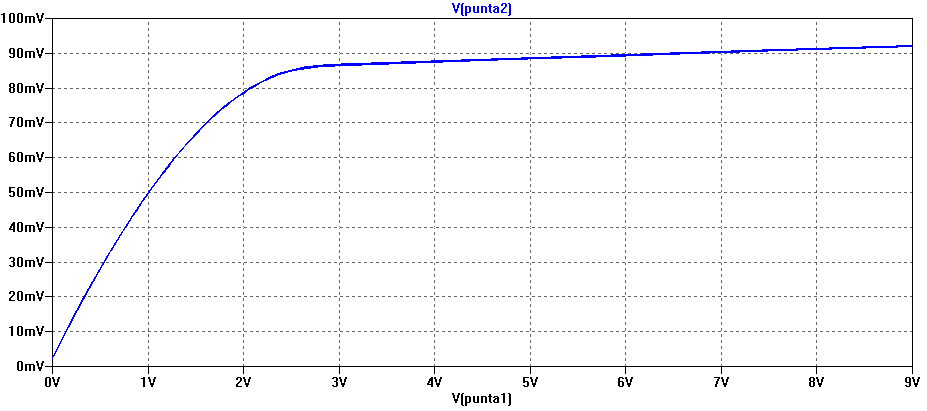
\includegraphics[scale=0.6]{simulaciones/2_vgs-15_sim.png}
\caption{Curva obtenida con $V_{GS} = -1.5\,\unit{V}$.}
\label{fig:simulacion_jfet_15}
\end{figure}

Para validar el método se comparará la curva obtenida con la que se obtiene realizando
un DC sweep de \emph{Spice}. En la figura \ref{fig:jfet_DCsweep} se muestra el circuito utilizado  para la simulación.

\begin{figure}[H]
\centering
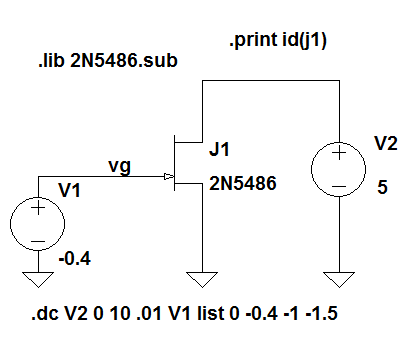
\includegraphics[scale=0.6]{circuitos/2_banco_dcsweep.png}
\caption{Circuito utilizado utilizando DC sweep.}
\label{fig:jfet_DCsweep}
\end{figure}

La curva obtenida se muestra en la figura \ref{fig:simulacion_jfet_dc_sweep}, se utilizaron
los mismos valores de $V_{GS} = \{\ 0.0\,\unit{V}\ ;\ -0.4\,\unit{V}\ ;\ -1.0\,\unit{V}\ ;\ -1.5\,\unit{V}\ \}$.

De la simulación se extraen los valores de $I_D$ para $V_{DS} = 5\,\unit{V}$. Obteniéndose aproximadamente:

\[ \displaystyle I_D = \{\ 22.5\,\unit{mA} \ ;\ 30.0\,\unit{mA} \ ;\ 42.0\,\unit{mA} \ ;\ 51.0\,\unit{mA} \ \} \]

Que concuerdan con los valores de $I_D$ obtenidos en las simulaciones del banco de medición 
que se utilizará en el laboratorio.

\begin{figure}[H]
\centering
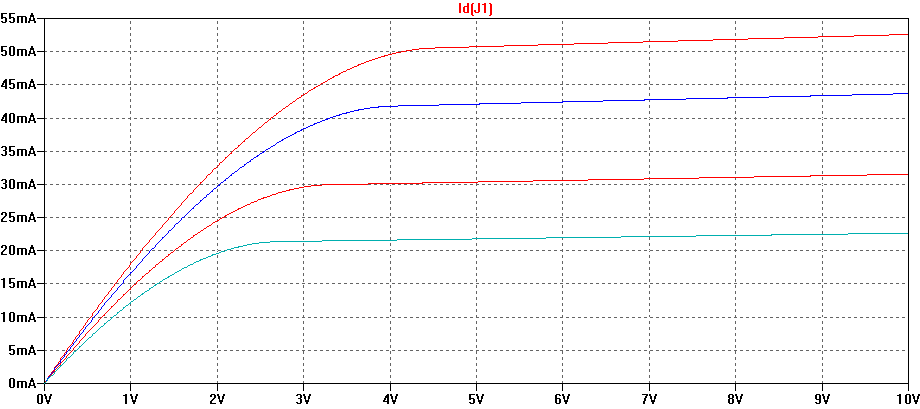
\includegraphics[scale=0.45]{simulaciones/2_sim_dcsweep.png}
\caption{Curva característica obtenida en \emph{Spice} utilizando DC sweep.}
\label{fig:simulacion_jfet_dc_sweep}
\end{figure}

\subsection{Mediciones}

Utilizando el banco de medición \ref{circuito:simulacion_jfet} a una frecuencia
de $f = 200\,\unit{Hz}$ se realizaron las mediciones utilizando un osciloscopio
en modo XY.

En las figuras \ref{fig:medicion_jfet_0}, \ref{fig:medicion_jfet_04},
\ref{fig:medicion_jfet_1} y \ref{fig:medicion_jfet_15} se muestran las curvas
obtenidas del osciloscopio para $V_{GS} = 0.0\,\unit{V}$, $V_{GS} = -0.4\,\unit{V}$,
$V_{GS} = -1.0\,\unit{V}$ y $V_{GS} = -1.5\,\unit{V}$ respectivamente.

\begin{figure}[H]
\centering
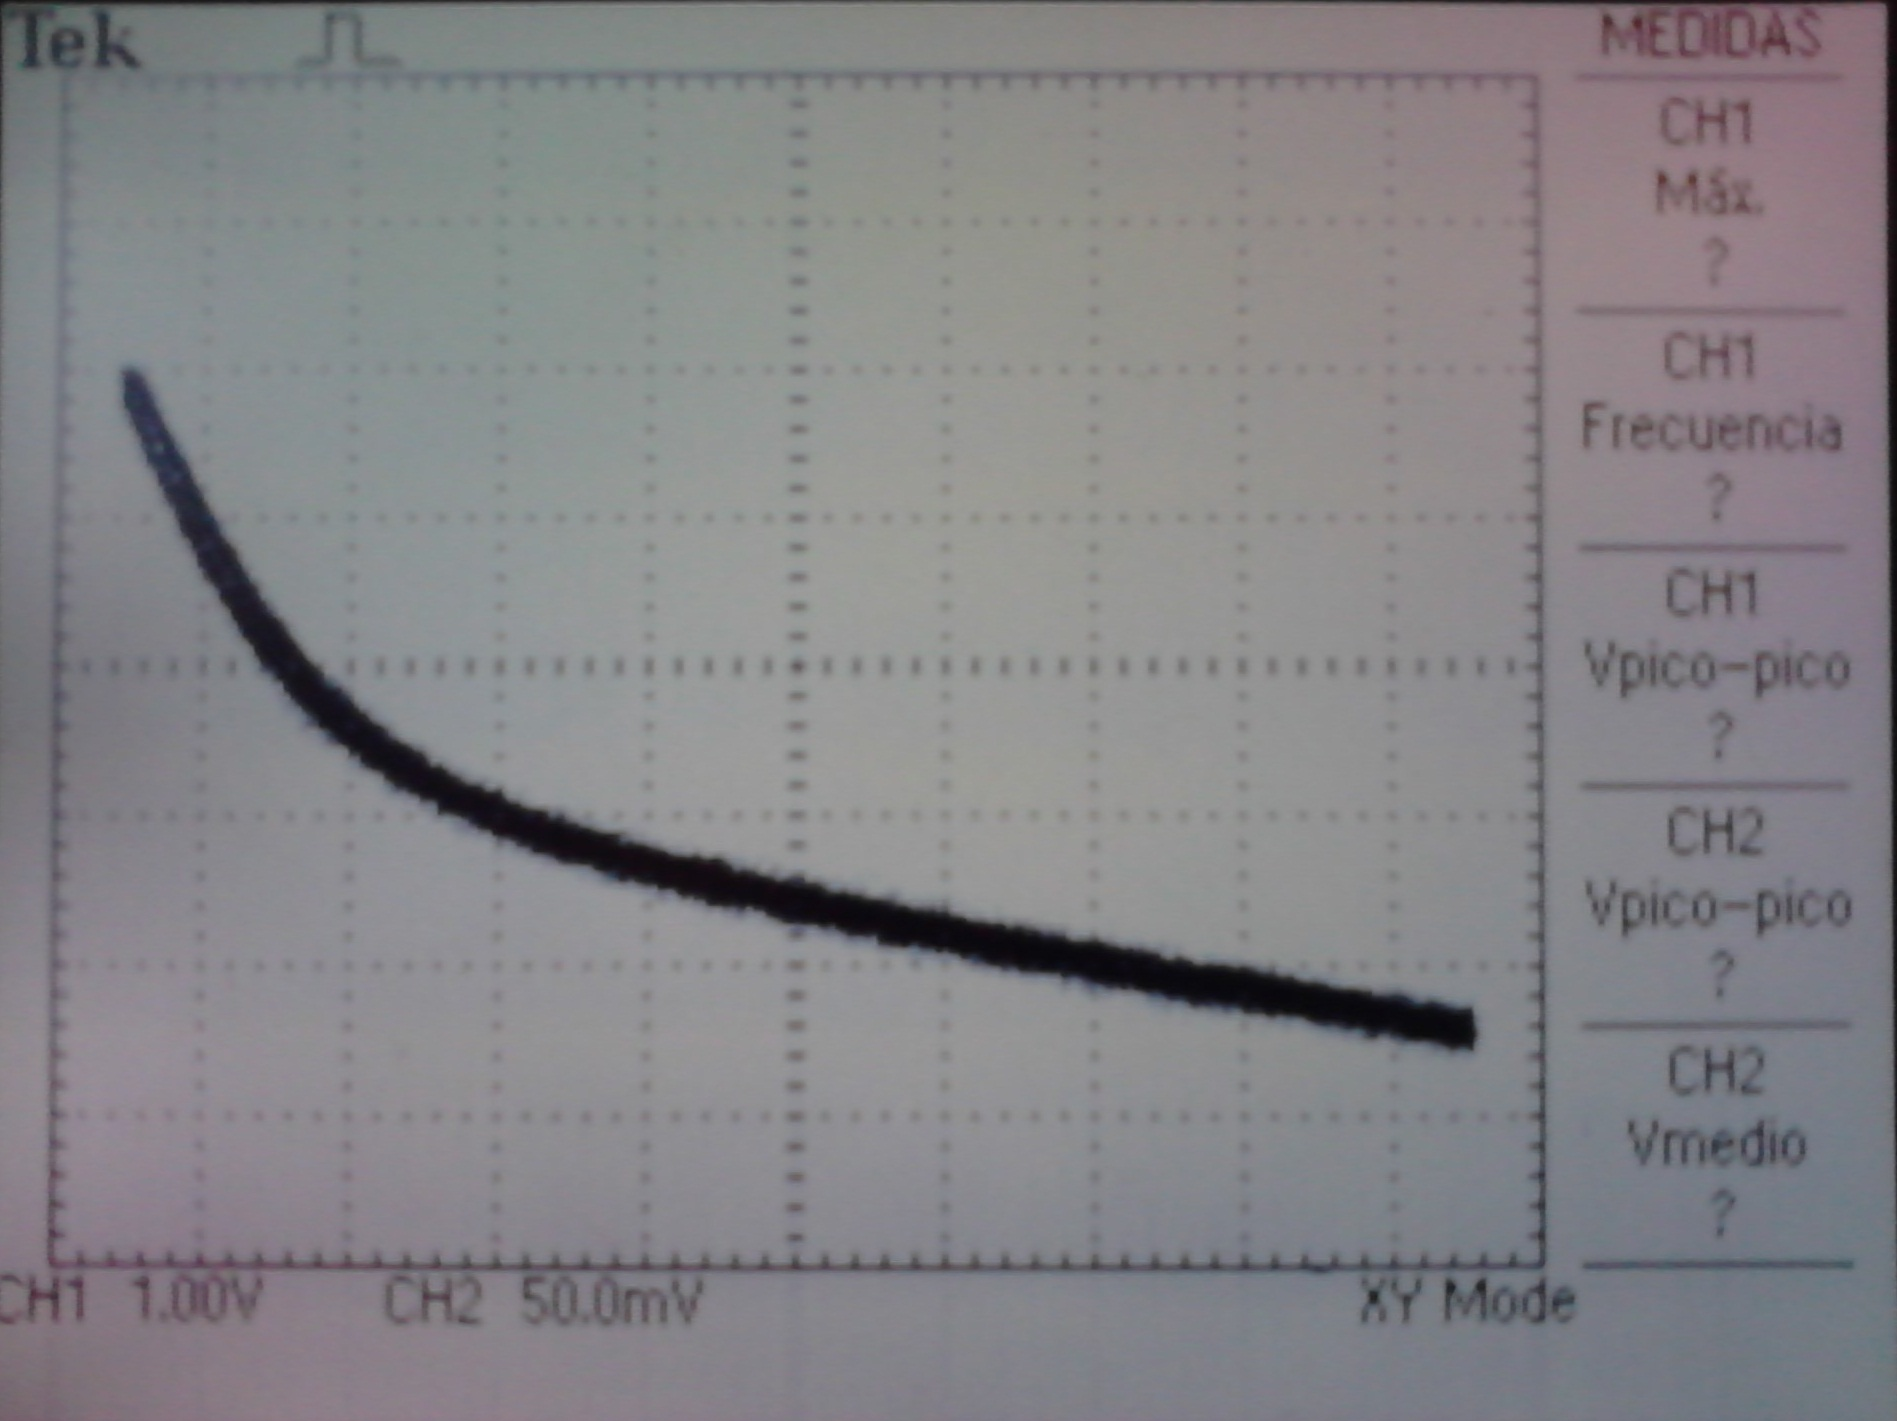
\includegraphics[scale=0.12]{mediciones/2_vgs0.jpg}
\caption{Curva obtenida con $V_{GS} = 0.0\,\unit{V}$.}
\label{fig:medicion_jfet_0}
\end{figure}

\begin{figure}[H]
\centering
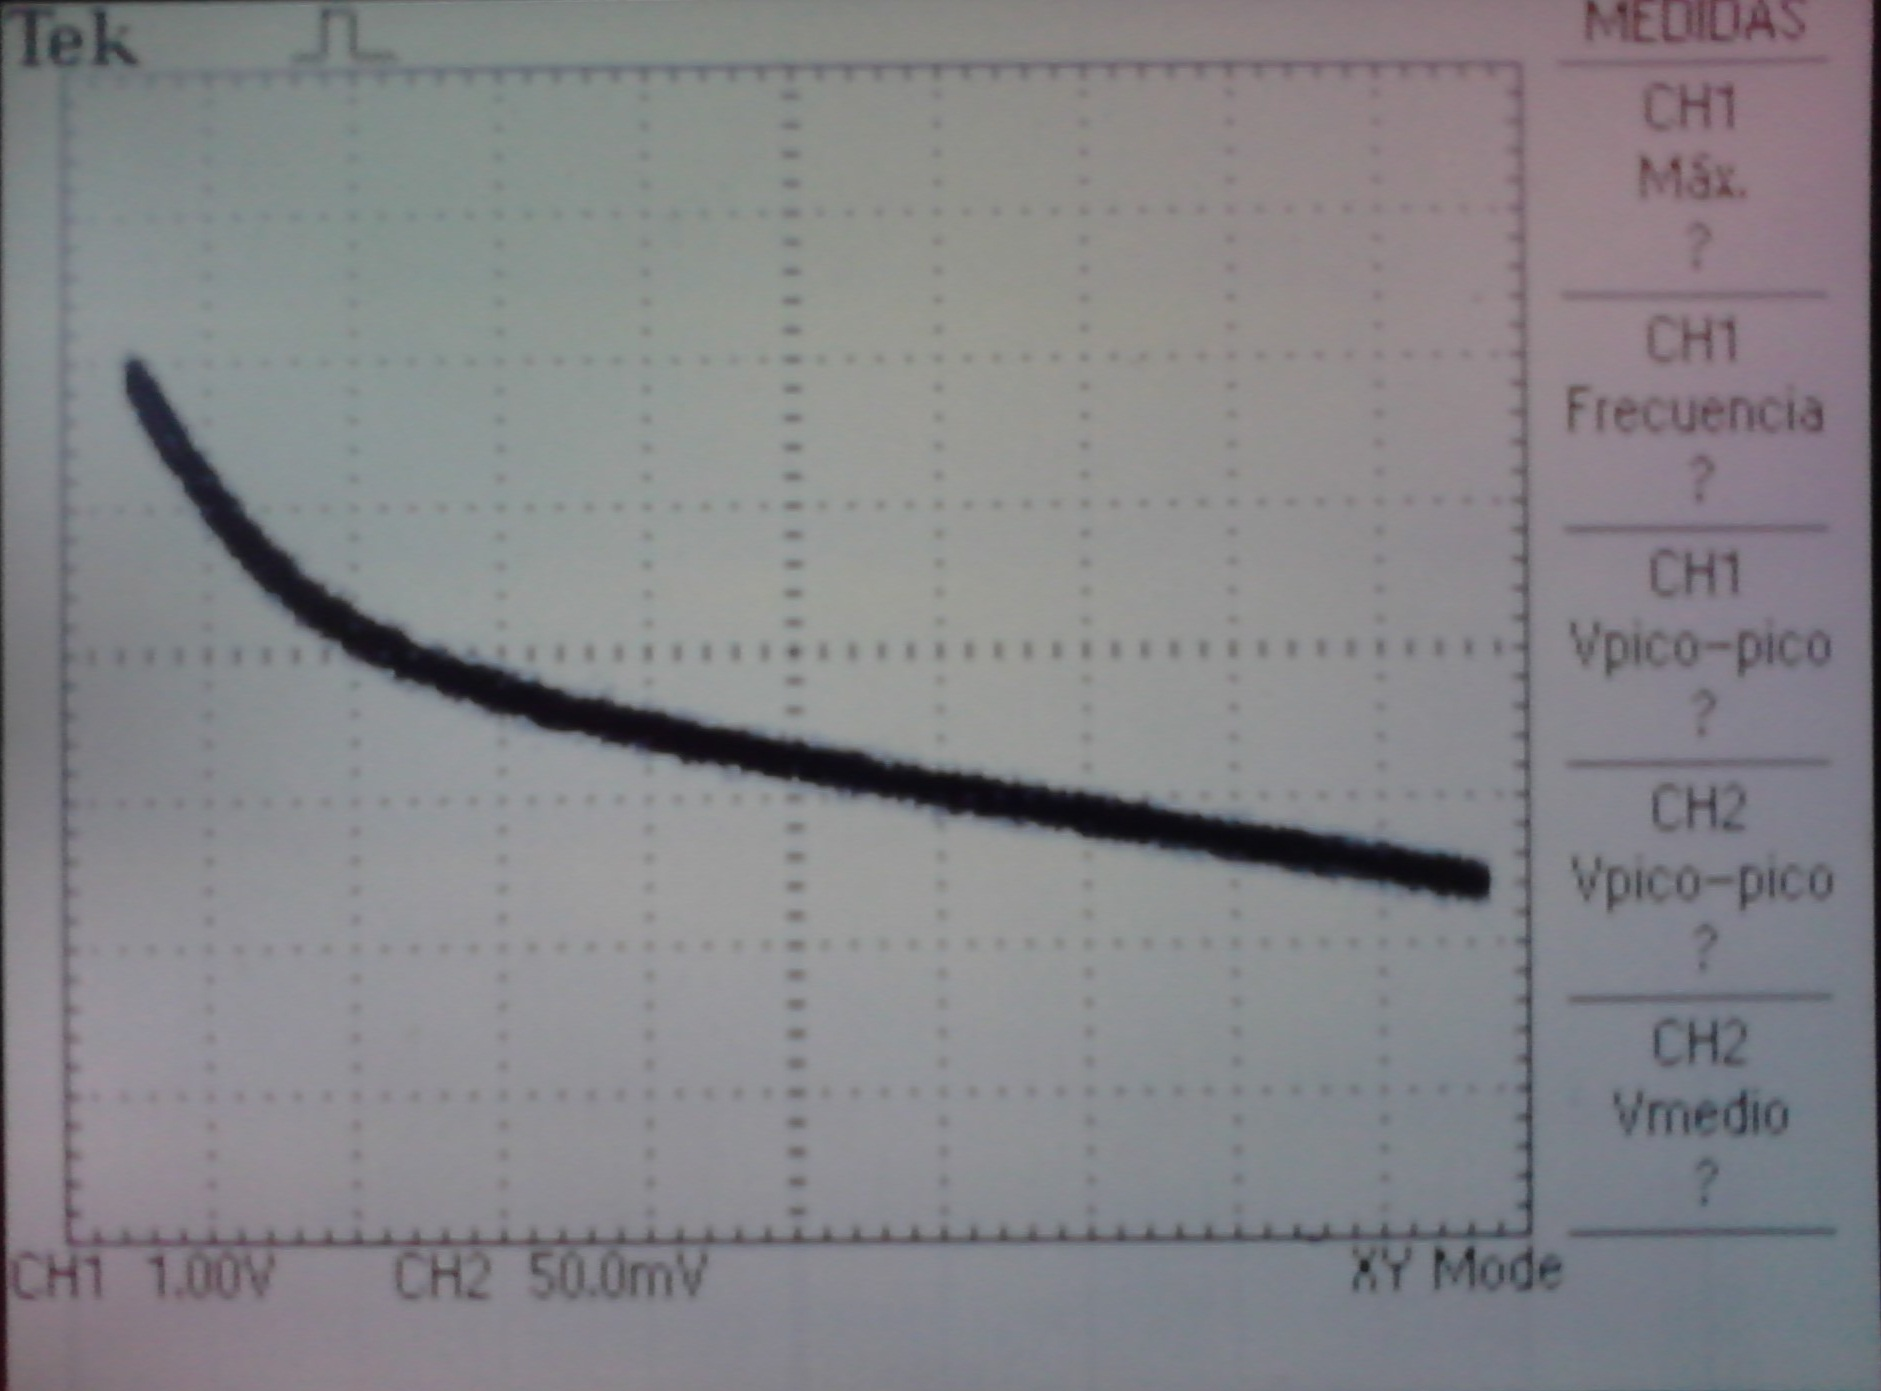
\includegraphics[scale=0.12]{mediciones/2_vgs-04.jpg}
\caption{Curva obtenida con $V_{GS} = -0.4\,\unit{V}$.}
\label{fig:medicion_jfet_04}
\end{figure}

\begin{figure}[H]
\centering
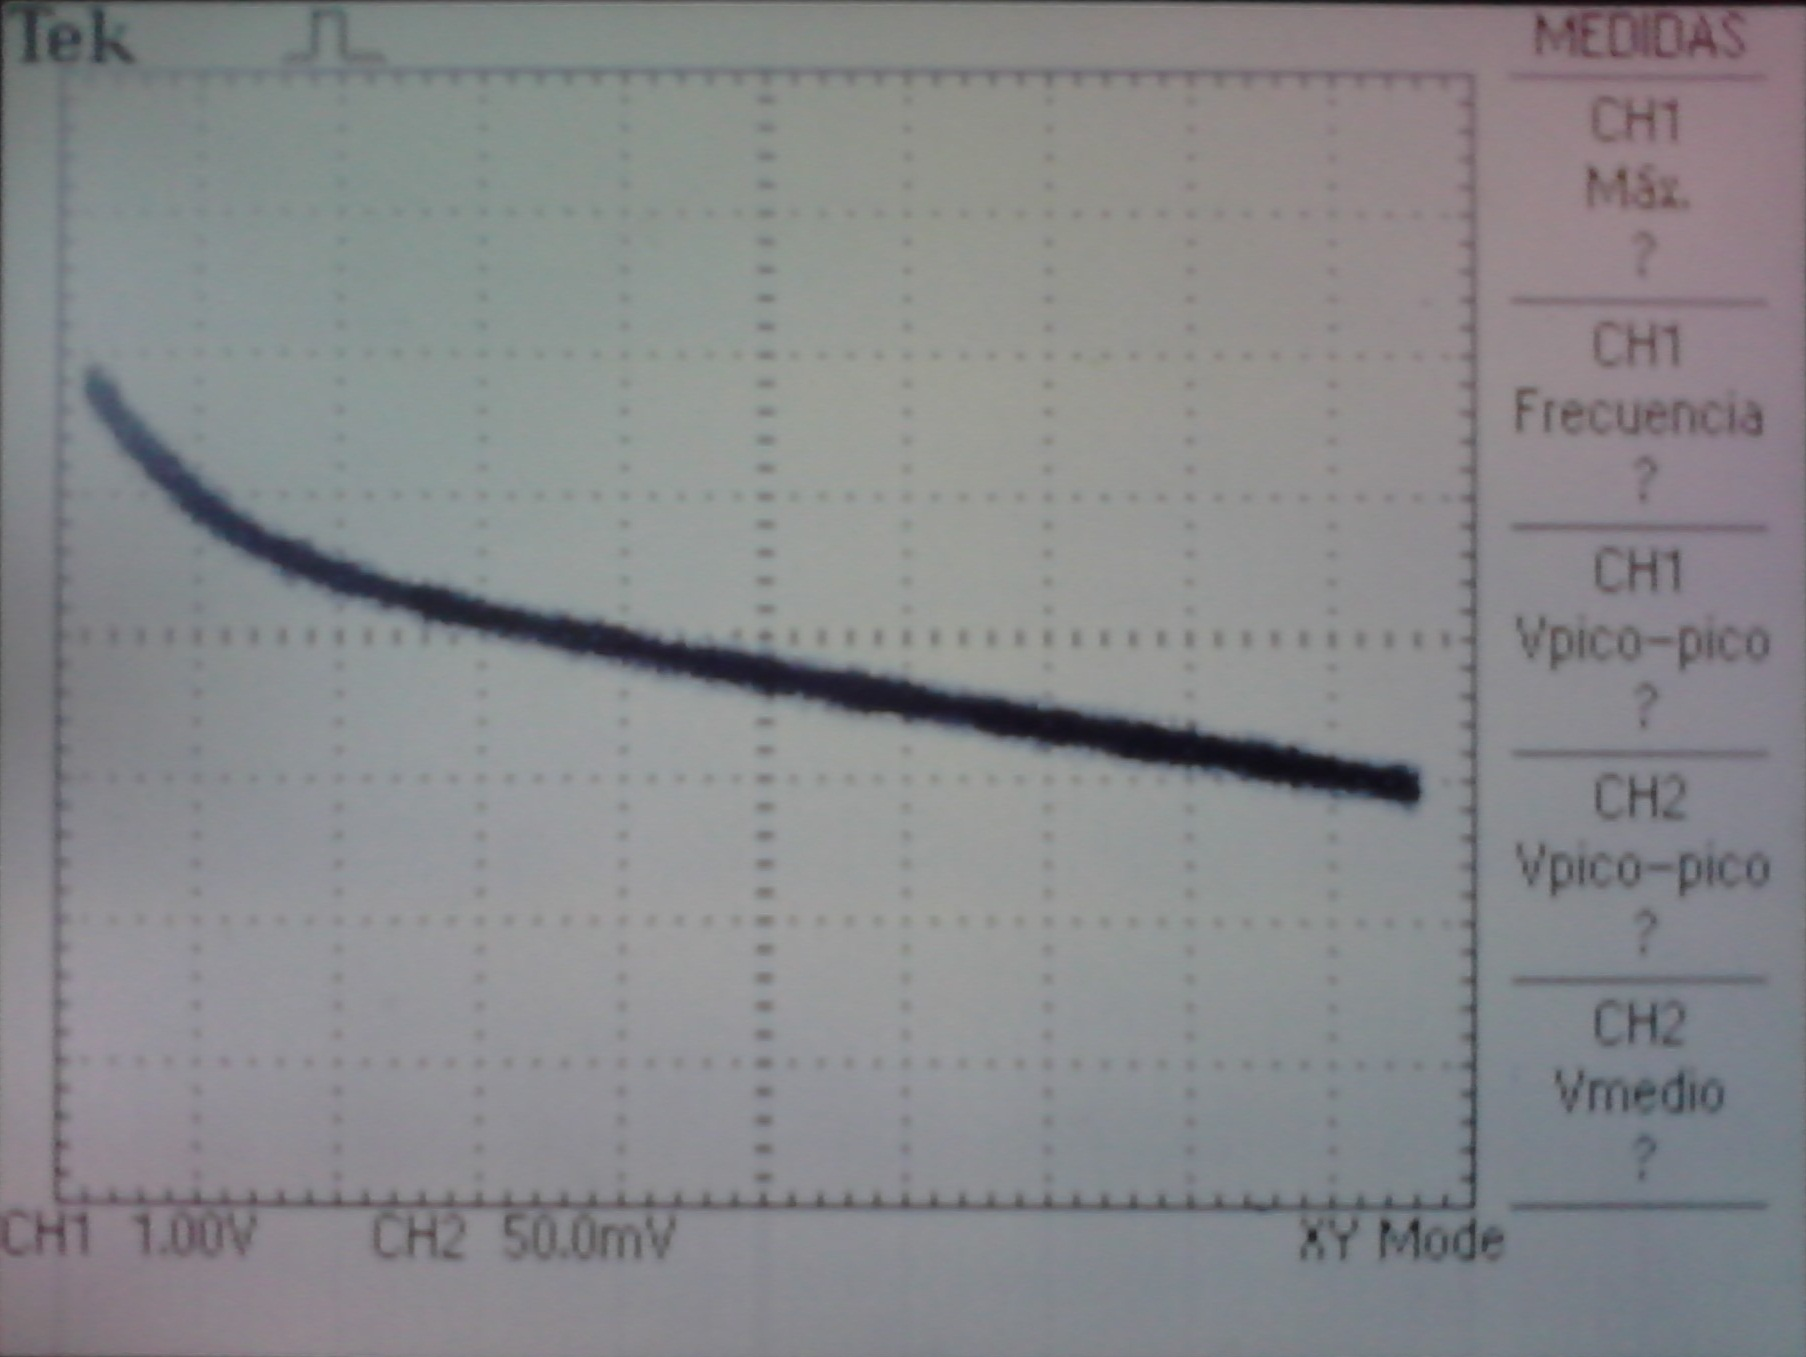
\includegraphics[scale=0.12]{mediciones/2_vgs-10.jpg}
\caption{Curva obtenida con $V_{GS} = -1.0\,\unit{V}$.}
\label{fig:medicion_jfet_1}
\end{figure}

\begin{figure}[H]
\centering
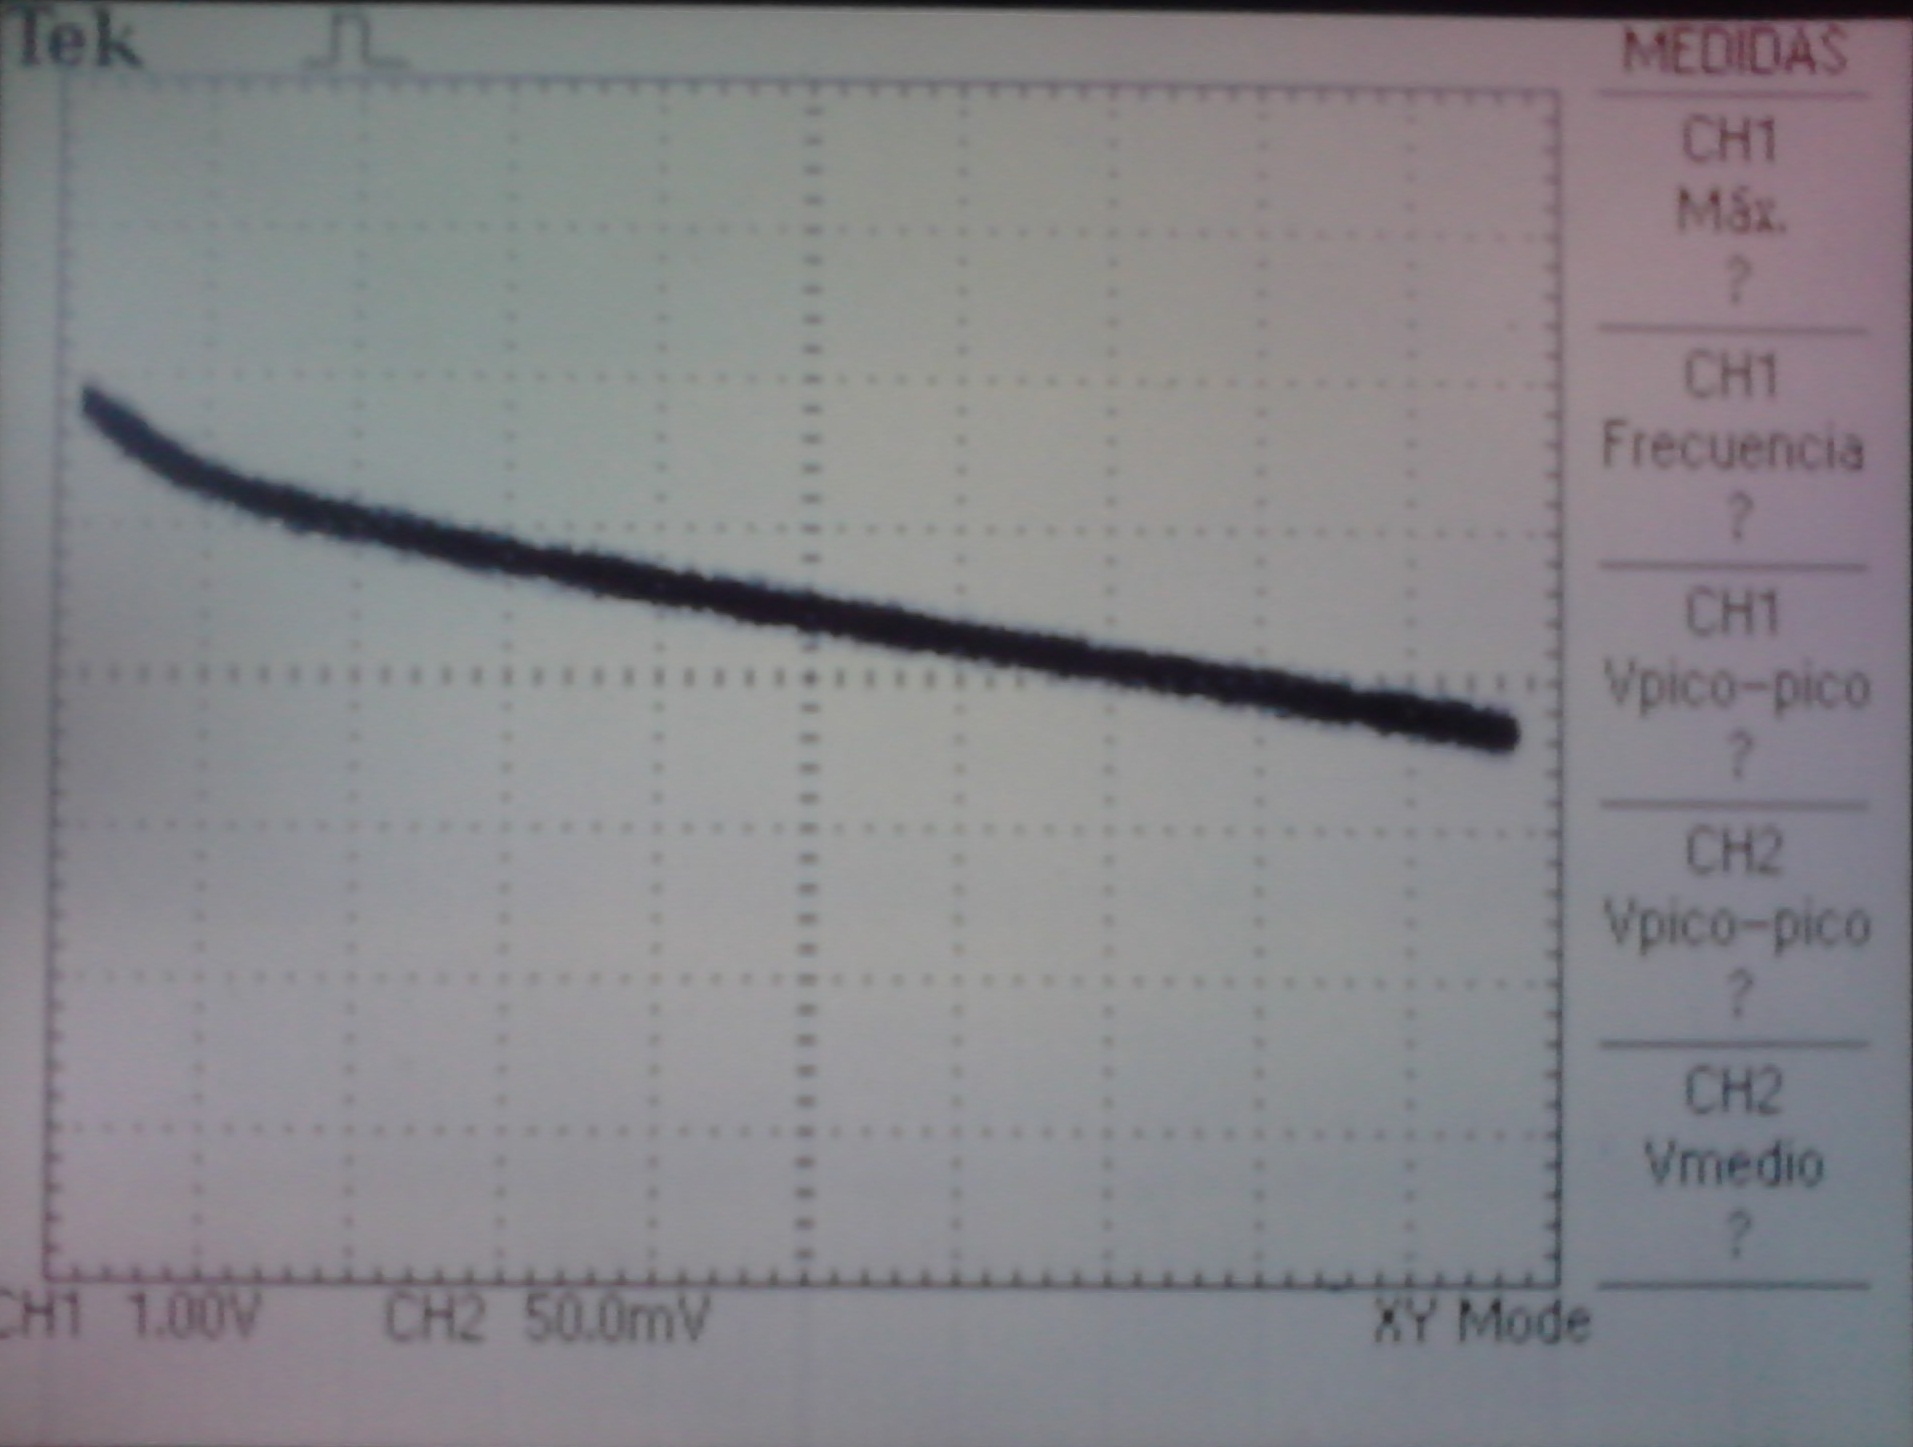
\includegraphics[scale=0.16]{mediciones/2_vgs-15.jpg}
\caption{Curva obtenida con $V_{GS} = -1.5\,\unit{V}$.}
\label{fig:medicion_jfet_15}
\end{figure}


Se obtiene aproximadamente $I_D$ para $V_{DS} = 5\,\unit{V}$ mediante la ecuacion \ref{eq:I_D_jfet}.

\[ \displaystyle I_D = \{\ 19.0\,\unit{mA} \ ;\ 30.8\,\unit{mA} \ ;\ 35.9\,\unit{mA} \ ;\ 46.2\,\unit{mA} \ \} \]

Los resultados obtenidos son similares a los obtenidos mediante simulación, 
destacando que las curvas obtenidas en las mediciones presentan un grosor
que impide medir con exactitud los valores medidos. Sin embargo
resultó ser un método útil para obtener la forma de las curvas.

\begin{table}[H]
\centering
\begin{tabular}{|c|c|c|c|}
\hline
$V_{GS}$ & $I_D$ simulado & $I_D$ medido  & Error simulado respecto a la medicion \\ \hline
$0.0\,\unit{V}$ & $22.5\,\unit{mA}$ & $19.0\,\unit{mA}$ & $18.4\,\unit{\%}$ \\ \hline
$-0.4\,\unit{V}$ & $30.0\,\unit{mA}$ & $30.8\,\unit{mA}$ & $-2.60\,\unit{\%}$ \\ \hline
$-1.0\,\unit{V}$ & $42.0\,\unit{mA}$ & $35.9\,\unit{mA}$ & $17.0\,\unit{\%}$ \\ \hline
$-1.5\,\unit{V}$ & $51.0\,\unit{mA}$ & $46.2\,\unit{mA}$ & $10.4\,\unit{\%}$ \\ \hline
\end{tabular}
\caption{Tabla comparativa de $I_D$ para distintos $V_{GS}$ con $V_{DS} = 5\,\unit{V}$.}
\label{table:2_comparacion_ID}
\end{table}

\section{Etapa amplificadora con dos transistores}

Se intercala una etapa en CC/DC (seguidor) entre el generador de señal
y la etapa amplificadora bajo análisis. Se tratará de mantener el mismo
valor de corriente de reposo en la etapa amplificadora. 

\subsection{Circuito seguidor}

En la figura \ref{fig:B_circuito} se muestra el circuito seguidor propuesto. Se utilizará el subíndice 1 para referirnos a la etapa seguidora.
Utiliza una configuración drain común y un transistor mosfet BS170
para mantener la misma tecnología que la etapa amplificadora.

En este caso la resistencia $R_L = 89\,\unit{k\Omega}$ se
despreciará ya que representa la resistencia interna de la etapa
amplificadora, que en paralelo a la resistencia $R_{S1}$ (que puede valer $470\,\unit{\Omega}$ o $1\,\unit{k\Omega}$) será
despreciable.

\begin{figure}[H]
\centering
\begin{circuitikz}[]\shorthandoff{>}
\draw 
(6,4.27) node[nigfete](nmos){}

(0,0) to [sV, l=$v_s$] (0,2) 
to [R, l=$R_s$] (0,4)
to [short] (1.5,4)
to [C, l=$C_{A1}$] (3,4)
to [short] (3,5)
to [R, l=$R_{G11}$] (3,7)
to [short] (6,7)
to [short] (nmos.D)

(3,0) to [R, l=$R_{G21}$] (3,4) 
to [short, *-] (nmos.G)
(nmos.S) to [R, l_=$R_{S1}$, v^=$v_O$, i=$i_{D1}$] (6,0)


(6,0) to [short, -*] (3,0)
to [short] (0,0)

(4.5, 7) to [short, -o] (4.5,7.5)  node[anchor=south] {$V_{DD}$}

(3,0) node[ground]{}

(nmos.G) node[anchor=south] {$G_1$}
(nmos.D) node[anchor=east] {$D_1$}
(nmos.S) node[anchor=west] {$S_1$}

(1,4) to [open, v=$v_i$] (1,0)
;\end{circuitikz}
\caption{Circuito seguidor propuesto}
\label{fig:B_circuito}
\end{figure}

En la tabla \ref{table:B_seguidor_datos} se muestran los datos del circuito, que son calculados
posteriormente.


\begin{table}[H]
\centering
\begin{tabular}{|c|c|} 
\hline
$V_{DD}$ & $28\,\unit{V}$ \\ \hline
$R_{G11}$ & $390\,\unit{k\Omega}$ \\ \hline
$R_{G21}$ & $100\,\unit{k\Omega}$ \\ \hline
$R_{S1}$ & $1\,\unit{k\Omega}$ \\ \hline
$R_{s}$ & $50\,\unit{\Omega}$ \\ \hline
\end{tabular}
\caption{Datos del circuito}
\label{table:B_seguidor_datos}
\end{table}

\subsubsection{Calculo de las resistencias de polarización}

Como se quitarán los resistores de polarización de la etapa amplificadora, se debe diseñar el seguidor de forma que
este la polarice.

Para esto es necesario obtener en continua una tensión 
de salida de $V_{O1} = V_{GG} = 3.04\,\unit{V}$.

A continuación se harán los cálculos necesarios para obtener las resistencias 
$R_{G11}$ y $R_{G21}$ del circuito utilizando los valores típicos
de $V_T$ y $K$:

Se obtiene la corriente $I_{DQ1}$ necesaria para obtener dicho $V_o$
fijando $R_S = 1\,\unit{k\Omega}$:

\[ \displaystyle I_{DQ1} = \frac{V_O}{R_{S1}} = 
\frac{3.04\,\unit{V}}{1\,\unit{k\Omega}} \approx 3.04\,\unit{mA} \]

De la ecuación número \ref{eq:A_mosfetid} se despeja y obtiene $V_{GS}$:

\[ \displaystyle V_{GS1} = \sqrt{\frac{I_{D1}\ 2}{K}} + V_T 
= \sqrt{\frac{3.04\,\unit{mA}\ 2}{123\,\unit{\frac{mA}{V^2}}}} + 2.1\,\unit{V} \approx 2.32\,\unit{V} \]

Por lo tanto la tensión en el gate del transistor respecto al común será:

\[ \displaystyle V_{G1} = V_{GS1} + V_{O1} = 
2.32\,\unit{V} + 3.04\, \unit{V} = 
5.36\,\unit{V} \]

De la ecuación número \ref{eq:B_Vgg} se fijó el valor de $R_{G21} = 100\,\unit{k\Omega}$ y se despeja $R_{G11}$.


\begin{equation}
V_{G1} = V_{DD}\frac{R_{G21}}{R_{G11}+R_{G21}} 
\label{eq:B_Vgg}
\end{equation}

Despejando $R_{G11}$:

\[ \displaystyle R_{G11} = R_{G21} \frac{V_{DD} - V_{G1}}{V_{G1}}
= 100\,\unit{k\Omega} \frac{28\,\unit{V} - 5.36\,\unit{V}}{5.36\,\unit{V}}
\approx 422\,\unit{k\Omega} \]

Se utilizará el valor mas cercano a los valores normalizados de resistencias. Por lo tanto:

\[ \displaystyle R_{G11} = 390\,\unit{k\Omega} \]

\subsubsection{Obtención del punto de reposo}

Con el valor de $R_{G11}$ calculado previamente se obtiene $V_{G1} = 5.7\,\unit{V}$.

A continuación se calcula el punto de reposo para 
las resistencias elegidas. 

De la malla de entrada se obtiene:

\begin{equation}
V_{G1} - V_{GS1} = I_{D1}\ R_{S1}
\label{eq:B_entrada}
\end{equation}

Mediante las ecuaciones \ref{eq:A_mosfetid} y \ref{eq:B_entrada}
se obtiene $V_{GS1} = 2.3\,\unit{V}$.

Se despeja y calcula $I_{D1}$ mediante la ecuación \ref{eq:B_entrada}:

\[ \displaystyle I_{D1} = \frac{V_{G1} - V_{GS1}}{R_{S1}} = 
\frac{5.7\,\unit{V} - 2.3\,\unit{V}}{1\,\unit{k\Omega}}
= 3.4\,\unit{mA} \]

Resultando:

\[ \displaystyle V_{O1} = V_{G1} - V_{GS1} 
= 5.7\,\unit{V} - 2.3\,\unit{V} 
= 3.4\,\unit{V} \]

Se calcula $V_{DSQ1}$:

\[ \displaystyle V_{DSQ1} = V_{DD} - V_{O1} = 28\,\unit{V} - 3.4\,\unit{V} = 24.5\,\unit{V} \]

Como $V_{DS1} > V_{GS1} - V_T$ el transistor se encuentra en saturación.

\[ \displaystyle (I_{DQ1};V_{DSQ1}) = (2.60\,\unit{mA};25.1\,\unit{V}) \]

En la tabla \ref{table:B_Q1_dispercion} se analiza la dispersión del
punto $Q1$ calculado para una variación del $30\%$ de los parámetros
$V_T$ y $K$ del transistor.
Para los valores límites el transistor sigue encontrándose en saturación.


\begin{table}[H]
\centering
\begin{tabular}{|c|c|c|c|} 
\hline
Parámetro & $V_{T}=1.47\,\unit{V}$ y $K=160\,\unit{\frac{mA}{V^2}}$ & 
$V_{T}=2.1\,\unit{V}$ y $K=123\,\unit{\frac{mA}{V^2}}$ &
$V_{T}=2.73\,\unit{V}$ y $K=86\,\unit{\frac{mA}{V^2}}$  \\ \hline
$I_{D1}$ & $4.1\,\unit{mA}$ & $3.4\,\unit{mA}$ & $2.8\,\unit{mA}$\\ \hline
$V_{DS1}$ & $23.9\,\unit{V}$ & $24.6\,\unit{V}$ & $25.2\,\unit{V}$\\ \hline
$V_{GS1}$ & $1.7\,\unit{V}$  &  $2.3\,\unit{V}$ & $3.0\,\unit{V}$\\ \hline
$V_{S1}$ & $4.1\,\unit{V}$ &  $3.4\,\unit{V}$ & $2.8\,\unit{V}$\\ \hline
$V_{G1}$ & $5.8\,\unit{V}$ &  $5.7\,\unit{V}$ & $5.8\,\unit{V}$\\ \hline
$V_{D1}$ & $28\,\unit{V}$ &  $28\,\unit{V}$ & $28\,\unit{V}$\\ \hline
\end{tabular}
\caption{Tabla comparativa de los puntos $Q1$ con la dispersión de los parámetros}
\label{table:B_Q1_dispercion}
\end{table}



\subsection{Circuito seguidor acoplado al amplificador}

En la figura \ref{fig:ByA} se muestra el circuito seguidor acoplado de forma
directa a la etapa amplificadora.\\



\begin{figure}[H]
\centering
\begin{circuitikz}[]\shorthandoff{>}
\draw 
(10,4.27) node[nigfete](nmosA){}

(6,7) to [short] (10,7)
to [R, l=$R_{D2}$] (nmosA.D)

(6,4) to [short, *-] (nmosA.G)
(nmosA.S) to [R, l=$R_{S2}$] (10,0)

(10,3) to [short, *-] (12,3) 
to [C, l=$C_S$] (12,0)

(10,5) to [short, *-] (12,5)
to [C, l=$C_{A2}$] (15,5)
to [R, l=$R_L$] (15,0)
to [short, -*] (12,0)
to [short, -*] (10,0)
to [short, -*] (6,0)
to [short] (4,0)

(6,7) to [short, *-o] (6,7.5)  node[anchor=south] {$V_{DD}$}

(10,0) node[ground]{}

(nmosA.G) node[anchor=south] {$G_2$}
(nmosA.D) node[anchor=east] {$D_2$}
(nmosA.S) node[anchor=east] {$S_2$}
(nmosA.B) node[anchor=west] {M2}

(1,5) to [open, v=$v_i$] (1,0)
(14,5) to [open, v=$v_o$] (14,0)


% etapa seguidora

(6,4.77) node[nigfete](nmosS){}

(0,0) to [sV, l=$v_s$] (0,2)
to [R, l=$R_s$] (0,4.5)
to [short] (1.5,4.5)
to [C, l=$C_{A1}$] (3,4.5)
to [short] (3,5)
to [R, l=$R_{G11}$] (3,7)
to [short] (6,7)
to [short] (nmos.D)

(3,0) to [R, l=$R_{G21}$] (3,4.5) 
to [short, *-] (nmosS.G)
(nmosS.S) to [R, l_=$R_{S1}$] (6,0)


(6,0) to [short, -*] (3,0)
to [short] (0,0)

(nmosS.G) node[anchor=south] {$G_1$}
(nmosS.D) node[anchor=east] {$D_1$}
(nmosS.S) node[anchor=east] {$S_1$}
(nmosS.B) node[anchor=west] {M1}

;\end{circuitikz}
\caption{Circuito seguidor con etapa amplificadora}
\label{fig:ByA}
\end{figure}


{\color{OliveGreen} 
Eliminar los resistores de polarización de la etapa original conectados 
al punto de acople ¿Por qué no tienen utilidad al conectar el seguidor en 
forma directa?}\\

El seguidor esta diseñado para que pueda polarizar la etapa amplificadora
al conectarlo de forma directa. Por esto se procuró obtener una tensión
de salida en continua igual a la tensión del gate respecto al común de la
etapa amplificadora ($V_{O1} = V_{G2}$). 

\subsubsection{Obtención del punto de reposo de la etapa amplificadora}

Partiendo del punto de reposo de la etapa seguidora se calcula el punto
de reposo de la etapa amplificadora. Recordando que la tensión de salida
de continua de la etapa seguidora es $V_{O1} = 3.5\,\unit{V}$ que será
la tensión de gate respecto al común del transistor M2 de la etapa
amplificadora. Por lo tanto $V_{G2} = 3.5\,\unit{V}$

De la malla de entrada se obtiene:

\begin{equation}
V_{G2} - V_{GS2} = I_{D2}\ R_{S2}
\label{eq:ByA_entrada_amplificadora}
\end{equation}

Mediante las ecuaciones \ref{eq:A_mosfetid} y \ref{eq:ByA_entrada_amplificadora}
se obtiene $V_{GS} = 2.24\,\unit{V}$.

Se despeja y calcula $I_D$ mediante la ecuación \ref{eq:ByA_entrada_amplificadora}:

\[ \displaystyle I_{D2} = \frac{V_{G2} - V_{GS2}}{R_{S2}} = 
\frac{3.4\,\unit{V} - 2.24\,\unit{V}}{1\,\unit{k\Omega}}
\approx 1.16\,\unit{mA} \]

Finalmente se calcula $V_{DS2}$:

\[ \displaystyle V_{DS2} = V_{DD} - I_{D2}(R_{D2} + R_{S2})
= 28\,\unit{V} - 1.16\,\unit{mA} (4.7\,\unit{k\Omega} + 1\,\unit{k\Omega})
\approx 21.4\,\unit{V} \]

En la tabla \ref{table:B_Q_acoplado} se muestran los distintos puntos
$Q2$ obtenidos de la etapa amplificadora, considerando la una dispersión del 30\% de los parámetros $K$ y $V_T$ del transistor.
En base a los valores de la tabla, el transistor estará en saturación
para los distintos puntos $Q2$ obtenidos considerando la dispersión
de los parámetros.

\begin{table}[H]
\centering
\begin{tabular}{|c|c|c|c|} 
\hline
Parámetro & $V_{T}=1.47\,\unit{V}$ y $K=160\,\unit{\frac{mA}{V^2}}$ & 
$V_{T}=2.1\,\unit{V}$ y $K=123\,\unit{\frac{mA}{V^2}}$ &
$V_{T}=2.73\,\unit{V}$ y $K=86\,\unit{\frac{mA}{V^2}}$ \\ \hline
$I_{D2}$ & $1.88\,\unit{mA}$ & $1.16\,\unit{mA}$ & $650\,\unit{\mu A}$\\ \hline
$V_{DS2}$ & $17.3\,\unit{V}$ & $21.4\,\unit{V}$ & $24.3\,\unit{V}$\\ \hline
$V_{GS2}$ & $1.62\,\unit{V}$  & $2.24\,\unit{V}$ & $2.85\,\unit{V}$\\ \hline 
$V_{S2}$ & $1.88\,\unit{V}$ &  $1.16\,\unit{V}$ & $0.65\,\unit{V}$\\ \hline
$V_{G2}$ & $3.5\,\unit{V}$ &  $3.4\,\unit{V}$ & $3.5\,\unit{V}$\\ \hline
$V_{D2}$ & $19.18\,\unit{V}$ &  $22.56\,\unit{V}$ & $24.95\,\unit{V}$\\ \hline
\end{tabular}
\caption{Tabla comparativa de los puntos $Q2$ de la etapa amplificadora}
\label{table:B_Q_acoplado}
\end{table}


\subsubsection{Obtención de parámetros}

A continuación se obtendrán los parámetros $A_v$, $R_i$ y $R_o$.
Para poder comparar sus diferencias con los calculados sin la
etapa seguidora.

En la figura \ref{fig:AyB_senial} se muestra modelo del circuito en señal.




\begin{figure}[H]
\centering
\begin{circuitikz}[]\shorthandoff{>}
\draw 
(10,4.27) node[nigfete](nmosA){}

(6,4) to [short, *-] (nmosA.G)
(nmosA.S) to [R, l_=$R_{S2}$, -*] (10,0)


(10,5) to [short] (16,5)
to [R, l_=$R_L$, v^=$v_o$] (16,0)

(13,5)to [R, l_=$R_{D2}$, *-*] (13,0)

(10,0) node[ground]{}

(nmosA.G) node[anchor=south] {$G_2$}
(nmosA.D) node[anchor=east] {$D_2$}
(nmosA.S) node[anchor=east] {$S_2$}
(nmosA.B) node[anchor=west] {M2}

% etapa seguidora

(6,4.77) node[nigfete](nmosS){}

(3,0) to [R, l_=$R_{G21}$, *-*] (3,4.5) 
(0,0) to [R, l_=$R_{G11}$, v^>=$v_i$] (0,4.5)
to (nmosS.G)

(5,4) to [open, v=$v_{gs}$] (5.8,3.5) 

(8,6) node[ground]{}
(nmos.D) to [short] (6,6) to [short] (8,6)

(nmosS.S) to [R, l^=$R_{S1}$, -*, v=$v_{s1}$, i=$i_{d1}$] (6,0)

(0,0) to [short] (16,0)


(nmosS.G) node[anchor=south] {$G_1$}
(nmosS.D) node[anchor=east] {$D_1$}
(nmosS.S) node[anchor=east] {$S_1$}
(nmosS.B) node[anchor=west] {M1}

;\end{circuitikz}
\caption{Modelo del circuito en señal}
\label{fig:AyB_senial}
\end{figure}

Se calculan los $gm$ de cada transistor mediante la ecuación \ref{eq:A_gm}

\[ \displaystyle g_{m1} = K(V_{GS1} - V_T) 
= 123\,\unit{\frac{mA}{V^2}} (2.3\,\unit{V} - 2.1\,\unit{V}) 
= 24.6\,\unit{\frac{mA}{V}}\]

\[ \displaystyle g_{m2} = K(V_{GS2} - V_T) 
= 123\,\unit{\frac{mA}{V^2}} (2.24\,\unit{V} - 2.1\,\unit{V}) 
= 17.22\,\unit{\frac{mA}{V}}\]

Se obtiene la amplificación de la etapa seguidora 

\[ \displaystyle A_{v1} = \frac{v_{s1}}{v_i} = 
\frac{i_{d1}\ R_{S1}}{i_{d1}\ R_{S1} + v_{gs1}} =
\frac{g_{m1}\ v_{gs1}\ R_{S1}}{g_{m1}\ v_{gs1}\ R_{S1} + v_{gs1}}\]


\begin{equation}
A_{v1} = \frac{g_{m1}\ R_{S1}}{g_{m1}\ R_{S1} + 1}
\label{eq:Av_seguidor}
\end{equation} 

Resultando:

\[ \displaystyle A_{v1} = \frac{24.6\,\unit{\frac{mA}{V}}\ 1\,\unit{k\Omega}}{24.6\,\unit{\frac{mA}{V}}\ 1\,\unit{k\Omega} + 1} 
\approx 0.96 \]

Se calcula la amplificación $A_{v2}$ de la etapa amplificadora mediante
la ecuación \ref{eq:A_Av}:

\[ \displaystyle A_{v2} = -g_{m2}(R_{D2}//R_L) =
-17.22\,\unit{\frac{mA}{V}}\ 3.2\,\unit{k\Omega}
\approx -55
\]


\[ \displaystyle A_v = \frac{v_o}{v_i}
= \frac{v_o}{v_i}\ \frac{v_{s1}}{v_{s1}}
= \frac{v_o}{v_{s1}}\ \frac{v_{s1}}{v_{i}}
= A_{v1}\ A_{v2}
= -55\ 0.96 = -52.8 \]

Se muestra en la tabla \ref{table:B_Av_dispersion}
los distintos parámetros obtenidos considerando una dispersión
del 30\% de los parámetros $V_T$ y $K$.

\begin{table}[H]
\centering
\begin{tabular}{|c|c|c|c|} 
\hline
Parámetro & $V_{T}=1.47\,\unit{V}$ y $K=160\,\unit{\frac{mA}{V^2}}$ & 
$V_{T}=1.82\,\unit{V}$ y $K=123\,\unit{\frac{mA}{V^2}}$ &
$V_{T}=2.73\,\unit{V}$ y $K=86\,\unit{\frac{mA}{V^2}}$  \\ \hline
$g_{m1}$ & $36.8\,\unit{\frac{mA}{V}}$ & $24.6\,\unit{\frac{mA}{V}}$ & $23.2\,\unit{\frac{mA}{V}}$\\ \hline
$g_{m2}$ & $24\,\unit{\frac{mA}{V}}$ & $17.22\,\unit{\frac{mA}{V}}$ & $10.32\,\unit{\frac{mA}{V}}$\\ \hline
$A_{v1}$ & 0.97 & 0.96 & 0.96 \\ \hline
$A_{v2}$ & -77 & -55 & -33 \\ \hline
$A_{v}$ & -75 & -53 & -32 \\ \hline
\end{tabular}
\caption{Tabla comparativa de la amplificación
considerando la dispersión de $V_T$ y $K$}
\label{table:B_Av_dispersion}
\end{table}


Las resistencias de entrada y salida del circuito son:

\[ \displaystyle R_i = (R_{G11} // R_{G21}) \approx 79\,\unit{k\Omega} \]

\[ \displaystyle R_o = R_{D2} = 4.70\,\unit{k\Omega} \]

\subsection{Simulaciones}

Se simuló mediante \emph{Spice} el circuito mostrado en la figura \ref{fig:ByA_circuito_spice}.
A continuación se muestran los resultados obtenidos en cada simulación.

\begin{figure}[H]
\centering
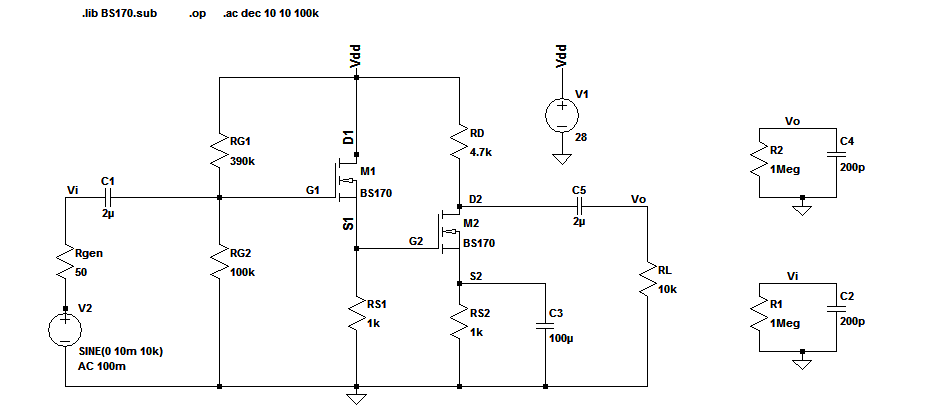
\includegraphics[scale=0.65]{circuitos/B_circuito_Av.png}
\caption{Banco de medición en \emph{Spice}}
\label{fig:ByA_circuito_spice}
\end{figure}

\subsubsection{Puntos de reposo}

En las tablas \ref{table:B_seguidor} y \ref{table:B_amplificador} se muestran los puntos 
de reposo de la etapa seguidora y amplificadora respectivamente, teniendo en cuenta una dispersión del 30\% de los parámetros $V_T$ y $K$.


\begin{table}[H]
\centering
\begin{tabular}{|c|c|c|c|} 
\hline
Parámetro & $V_{T}=1.47\,\unit{V}$ y $K=160\,\unit{\frac{mA}{V^2}}$ & 
$V_{T}=1.82\,\unit{V}$ y $K=123\,\unit{\frac{mA}{V^2}}$ &
$V_{T}=2.73\,\unit{V}$ y $K=86\,\unit{\frac{mA}{V^2}}$ \\ \hline
$I_{D1Q}$ & $4.01\,\unit{mA}$ & $2.85\,\unit{mA}$ & $2.73\,\unit{mA}$\\ \hline
$V_{DS1Q}$ & $24.0\,\unit{V}$ & $21.1\,\unit{V}$ & $25.3\,\unit{V}$\\ \hline
$V_{GS1Q}$ & $1.70\,\unit{V}$  & $2.04\,\unit{V}$ & $2.99\,\unit{V}$\\ \hline
\end{tabular}
\caption{Tabla comparativa de los puntos $Q1$ de la etapa seguidora obtenidos en \emph{Spice}}
\label{table:B_seguidor}
\end{table}


\begin{table}[H]
\centering
\begin{tabular}{|c|c|c|c|} 
\hline
Parámetro & $V_{T}=1.47\,\unit{V}$ y $K=160\,\unit{\frac{mA}{V^2}}$ & 
$V_{T}=1.82\,\unit{V}$ y $K=123\,\unit{\frac{mA}{V^2}}$ &
$V_{T}=2.73\,\unit{V}$ y $K=86\,\unit{\frac{mA}{V^2}}$ \\ \hline
$I_{D2Q}$ & $2.37\,\unit{mA}$ & $908\,\unit{\mu A}$ & $56\,\unit{pA}$\\ \hline
$V_{DS2Q}$ & $14.5\,\unit{V}$ & $18.8\,\unit{V}$ & $28.0\,\unit{V}$\\ \hline
$V_{GS2Q}$ & $1.65\,\unit{V}$  & $1.95\,\unit{V}$ & $2.73\,\unit{V}$\\ \hline
\end{tabular}
\caption{Tabla comparativa de los puntos $Q2$ de la etapa amplificadora obtenidos en \emph{Spice}}
\label{table:B_amplificador}
\end{table}

De la tabla \ref{table:B_amplificador} se observa que la etapa amplificadora está
en corto. Por lo que la amplificación será nula.
Se procede a disminuir el valor de $R_{G11}$ a un valor normalizado menor, para
poder aumentar $V_{G1}$ y verificar que para $V_{Tmax}$ y $K_{min}$ la etapa
amplificadora no esté en corte.
Se utilizará el siguiente valor de  $R_{G11} = 330\,\unit{k\Omega}$.

Se vuelve a simular en \emph{Spice} considerando la dispersión de los parámetros
con la modificación realizada. En las tablas \ref{table:B_seguidor_modificado} y \ref{table:B_amplificador_modificado} se muestran los puntos 
de reposo de la etapa seguidora y amplificadora respectivamente.
Se verifica que para todos los posibles casos $V_{DS} > V_{GS} - V_T$ para ambos transistores, por lo tanto están en saturación.

\begin{table}[H]
\centering
\begin{tabular}{|c|c|c|c|} 
\hline
Parámetro & $V_{T}=1.47\,\unit{V}$ y $K=160\,\unit{\frac{mA}{V^2}}$ & 
$V_{T}=1.82\,\unit{V}$ y $K=123\,\unit{\frac{mA}{V^2}}$ &
$V_{T}=2.73\,\unit{V}$ y $K=86\,\unit{\frac{mA}{V^2}}$ \\ \hline
$I_{D1Q}$ & $4.79\,\unit{mA}$ & $4.42\,\unit{mA}$ & $3.49\,\unit{mA}$\\ \hline
$V_{DS1Q}$ & $23.1\,\unit{V}$ & $23.6\,\unit{V}$ & $24.5\,\unit{V}$\\ \hline
$V_{GS1Q}$ & $1.72\,\unit{V}$  & $2.09\,\unit{V}$ & $3.02\,\unit{V}$\\ \hline
$V_{S1}$ & $4.79\,\unit{V}$  & $4.42\,\unit{V}$ & $3.49\,\unit{V}$\\ \hline
$V_{G1}$ & $6.51\,\unit{V}$  & $6.51\,\unit{V}$ & $6.51\,\unit{V}$\\ \hline
$V_{D1}$ & $28\,\unit{V}$  & $28\,\unit{V}$ & $28\,\unit{V}$\\ \hline
\end{tabular}
\caption{punto $Q1$ de la etapa seguidora obtenidos en \emph{Spice} con $R_{G11} = 330\,\unit{k\Omega}$}
\label{table:B_seguidor_modificado}
\end{table}

\begin{table}[H]
\centering
\begin{tabular}{|c|c|c|c|} 
\hline
Parámetro & $V_{T}=1.47\,\unit{V}$ y $K=160\,\unit{\frac{mA}{V^2}}$ & 
$V_{T}=1.82\,\unit{V}$ y $K=123\,\unit{\frac{mA}{V^2}}$ &
$V_{T}=2.73\,\unit{V}$ y $K=86\,\unit{\frac{mA}{V^2}}$ \\ \hline
$I_{D2Q}$ & $3.12\,\unit{mA}$ & $2.40\,\unit{mA}$ & $638\,\unit{\mu A}$\\ \hline
$V_{DS2Q}$ & $10.2\,\unit{V}$ & $14.3\,\unit{V}$ & $24.4\,\unit{V}$\\ \hline
$V_{GS2Q}$ & $1.67\,\unit{V}$  & $2.02\,\unit{V}$ & $2.85\,\unit{V}$\\
\hline
$V_{S2}$ & $3.12\,\unit{V}$  & $2.40\,\unit{V}$ & $0.638\,\unit{V}$\\ \hline
$V_{G2}$ & $4.79\,\unit{V}$  & $4.42\,\unit{V}$ & $3.49\,\unit{V}$\\ \hline
$V_{D2}$ & $13.3\,\unit{V}$  & $16.7\,\unit{V}$ & $25.0\,\unit{V}$\\ \hline
\end{tabular}
\caption{Punto $Q2$ de la etapa amplificadora obtenidos en \emph{Spice} con $R_{G11} = 330\,\unit{k\Omega}$}
\label{table:B_amplificador_modificado}
\end{table}



\subsubsection{Amplificación}

Se simuló el circuito mostrado en la figura \ref{fig:ByA_circuito_spice} para
obtener la amplificación del circuito.

En las figuras \ref{fig:AyB_av_tipico}, \ref{fig:AyB_av_min} y \ref{fig:AyB_av_max} 
se muestran la respuesta en frecuencia de la amplificacion típica, mínima y máxima considerando una dispersión
del 30\% de los parámetros $V_T$ y $K$.
Se observa que la amplificación deseada $A_v = -50$ se encuentra dentro del 
rango de posibles valores de $A_v = [-95;-31]$ simulados.

\begin{figure}[H]
\centering
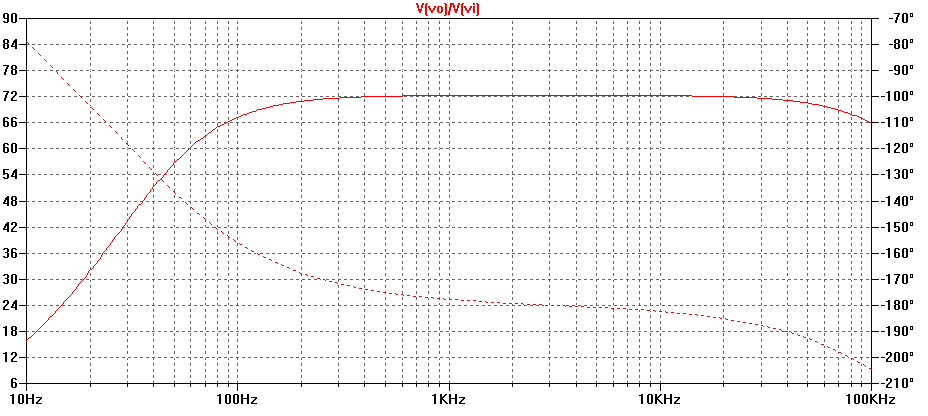
\includegraphics[scale=0.5]{simulaciones/B_av_tipica.png}
\caption{Amplificación del circuito típica}
\label{fig:AyB_av_tipico}
\end{figure}

\begin{figure}[H]
\centering
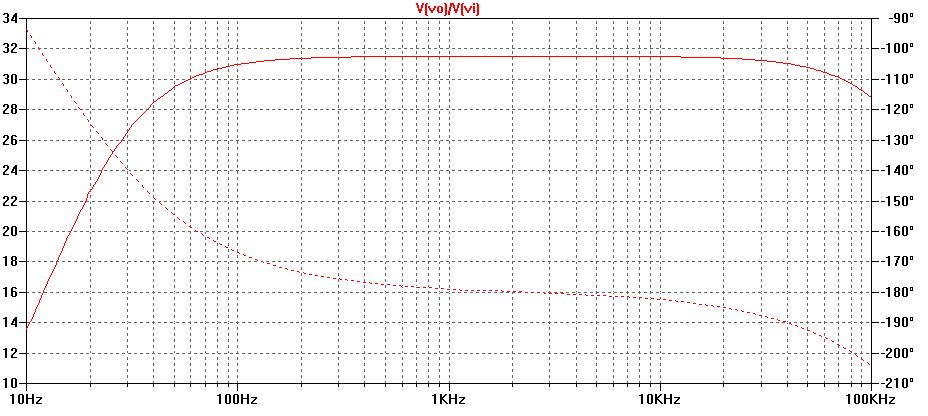
\includegraphics[scale=0.5]{simulaciones/B_av_min.png}
\caption{Amplificación del circuito mínima}
\label{fig:AyB_av_min}
\end{figure}

\begin{figure}[H]
\centering
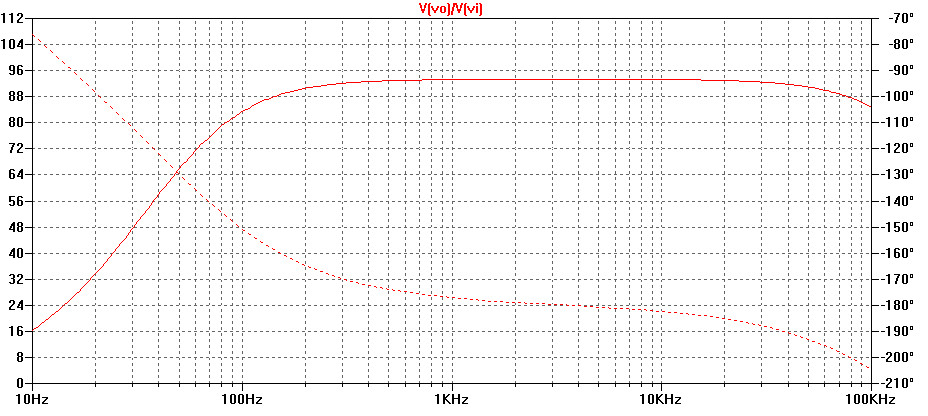
\includegraphics[scale=0.5]{simulaciones/B_av_max.png}
\caption{Amplificación del circuito máxima}
\label{fig:AyB_av_max}
\end{figure}


\subsubsection{Resistencia de entrada}

Se simuló el circuito mostrado en la figura \ref{fig:B_banco_Ri}.
Conectando una fuente de prueba $v_p$ en la entrada en serie a un
resistor de $47\,\unit{k\Omega}$. Se utilizó esta configuración
para la simulación ya que será el mismo banco de medición que
se utilizará para las mediciones.
Se obtiene la resistencia de entrada mediante $R_i = \frac{v_p}{i_p}$.

\begin{figure}[H]
\centering
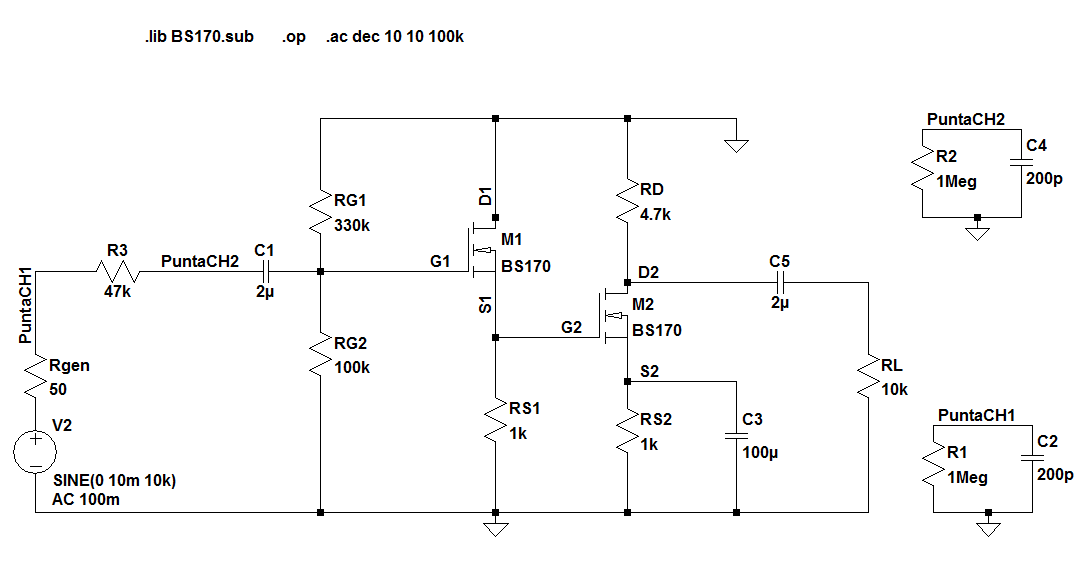
\includegraphics[scale=0.45]{circuitos/B_banco_Ri.png}
\caption{Banco de medición para la obtención de $R_i$}
\label{fig:B_banco_Ri}
\end{figure}

En la figura \ref{fig:B_Ri} se muestra valor
de la resistencia de entrada $R_i$ para distintas frecuencias.
Que para la frecuencia de trabajo $f=1\,\unit{kHz}$ se obtiene
un valor de $R_i \approx 72\,\unit{k\Omega}$.

\begin{figure}[H]
\centering
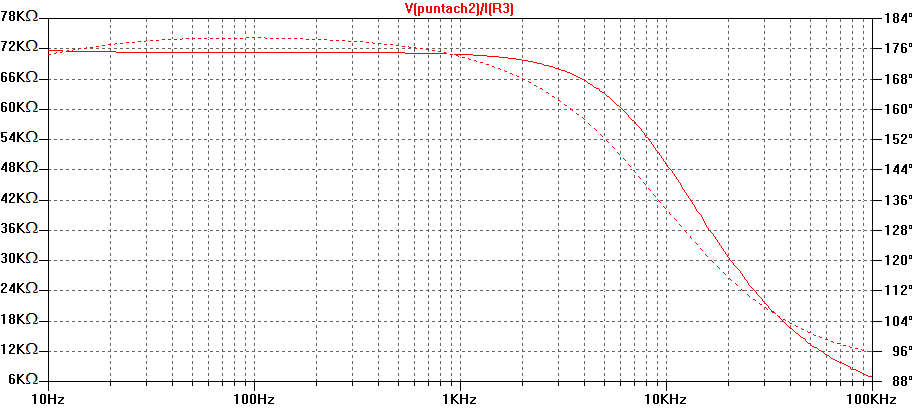
\includegraphics[scale=0.5]{simulaciones/B_sim_Ri.png}
\caption{Resistencia de entrada $R_i$ en frecuencia}
\label{fig:B_Ri}
\end{figure}

\subsubsection{Resistencia de salida}

En la figura \ref{fig:B_banco_Ro} se muestra el banco de medición utilizado para
la obtención de $R_o$.
Al igual que para $R_i$, se conecta una fuente de prueba $v_p$ en la salida en serie
a un resistor de $4.7\,\unit{k\Omega}$ y se obtiene la resistencia de salida mediante $R_o = \frac{v_p}{i_p}$.

\begin{figure}[H]
\centering
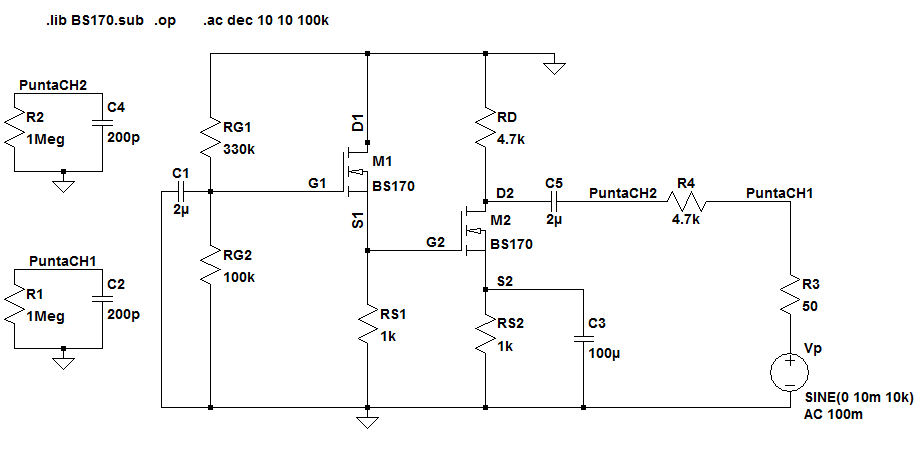
\includegraphics[scale=0.65]{circuitos/B_banco_Ro.png}
\caption{Banco de medición para la obtención de $R_o$}
\label{fig:B_banco_Ro}
\end{figure}

En la figura \ref{fig:B_Ro} se muestra el valor
de la resistencia de salida $R_o$.
Que para la frecuencia de trabajo $f=1\,\unit{kHz}$ se obtiene
un valor de $R_o \approx 4.68\,\unit{k\Omega}$.

\begin{figure}[H]
\centering
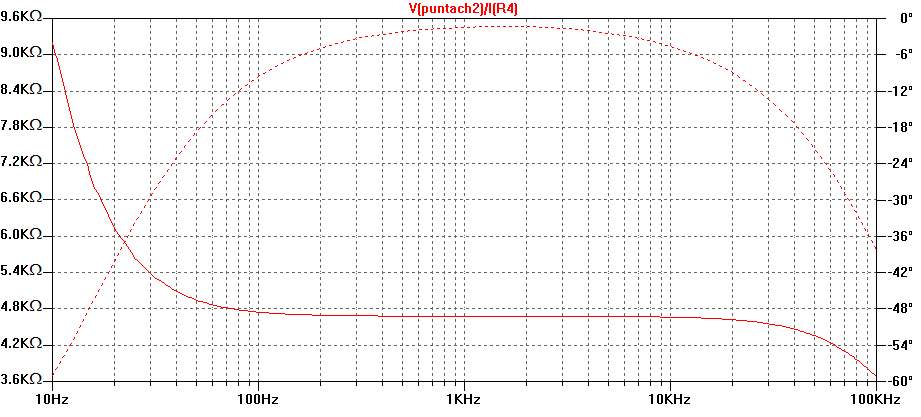
\includegraphics[scale=0.5]{simulaciones/B_sim_Ro.png}
\caption{Resistencia de entrada $R_o$ en frecuencia}
\label{fig:B_Ro}
\end{figure}

\subsection{Cálculo por inspección del circuito modificado}

Se volverán a obtener los parámetros calculados por inspección debido a la 
modificación de $R_{G1}$ a $R_{G1} = 330\,\unit{k\Omega}$ en las simulaciones realizadas. Para poder
comparar los resultados calculados con la simulación y la medición.

\subsubsection{Punto de reposo}

En las tablas \ref{table:B_calculo_modificado_seguidor} y \ref{table:B_calculo_modificado_amplificador}
se muestran los puntos de reposo de la etapa seguidora y amplificadora, respectivamente. Considerando
una dispersión del $30\%$ de los parámetros $V_T$ y $K$.

\begin{table}[H]
\centering
\begin{tabular}{|c|c|c|c|} 
\hline
Parámetro & $V_{T}=1.47\,\unit{V}$ y $K=160\,\unit{\frac{mA}{V^2}}$ & 
$V_{T}=2.10\,\unit{V}$ y $K=123\,\unit{\frac{mA}{V^2}}$ &
$V_{T}=2.73\,\unit{V}$ y $K=86\,\unit{\frac{mA}{V^2}}$ \\ \hline
$I_{D1Q}$ & $4.79\,\unit{mA}$ & $4.14\,\unit{mA}$ & $3.49\,\unit{mA}$\\ \hline
$V_{DS1Q}$ & $23.2\,\unit{V}$ & $23.9\,\unit{V}$ & $24.5\,\unit{V}$\\ \hline
$V_{GS1Q}$ & $1.71\,\unit{V}$  & $2.36\,\unit{V}$ & $3.01\,\unit{V}$\\ \hline
$V_{S1}$ & $4.79\,\unit{V}$  & $4.14\,\unit{V}$ & $3.49\,\unit{V}$\\ \hline
$V_{G1}$ & $6.51\,\unit{V}$  & $6.51\,\unit{V}$ & $6.51\,\unit{V}$\\ \hline
$V_{D1}$ & $28\,\unit{V}$  & $28\,\unit{V}$ & $28\,\unit{V}$\\ \hline
\end{tabular}
\caption{Punto $Q1$ de la etapa seguidora obtenidos mediante inspección con $R_{G11} = 330\,\unit{k\Omega}$}
\label{table:B_calculo_modificado_seguidor}
\end{table}

\begin{table}[H]
\centering
\begin{tabular}{|c|c|c|c|} 
\hline
Parámetro & $V_{T}=1.47\,\unit{V}$ y $K=160\,\unit{\frac{mA}{V^2}}$ & 
$V_{T}=2.10\,\unit{V}$ y $K=123\,\unit{\frac{mA}{V^2}}$ &
$V_{T}=2.73\,\unit{V}$ y $K=86\,\unit{\frac{mA}{V^2}}$ \\ \hline
$I_{D2Q}$ & $3.12\,\unit{mA}$ & $1.87\,\unit{mA}$ & $640\,\unit{\mu A}$\\ \hline
$V_{DS2Q}$ & $10.2\,\unit{V}$ & $17.2\,\unit{V}$ & $24.4\,\unit{V}$\\ \hline
$V_{GS2Q}$ & $1.67\,\unit{V}$  & $2.27\,\unit{V}$ & $2.85\,\unit{V}$\\ \hline
$V_{S2}$ & $3.12\,\unit{V}$  & $1.87\,\unit{V}$ & $640\,\unit{mV}$\\ \hline
$V_{G2}$ & $4.79\,\unit{V}$  & $4.14\,\unit{V}$ & $3.49\,\unit{V}$\\ \hline
$V_{D2}$ & $13.3\,\unit{V}$  & $19.1\,\unit{V}$ & $25.0\,\unit{V}$\\ \hline
\end{tabular}
\caption{Punto $Q2$ de la etapa amplificadora obtenidos mediante inspección con $R_{G11} = 330\,\unit{k\Omega}$}
\label{table:B_calculo_modificado_amplificador}
\end{table}

\subsubsection{Parámetros del circuito}

Se vuelve a calcular los parámetros del circuito para el nuevo
valor de $R_{G11}$ de la etapa seguidora.
En la tabla \ref{table:B_modificado_Av_dispersion} se muestran
los distintos parámetros obtenidos considerando una dispersión
del 30\% de los parámetros $V_T$ y $K$.

\begin{table}[H]
\centering
\begin{tabular}{|c|c|c|c|} 
\hline
Parámetro & $V_{T}=1.47\,\unit{V}$ y $K=160\,\unit{\frac{mA}{V^2}}$ & 
$V_{T}=1.82\,\unit{V}$ y $K=123\,\unit{\frac{mA}{V^2}}$ &
$V_{T}=2.73\,\unit{V}$ y $K=86\,\unit{\frac{mA}{V^2}}$  \\ \hline
$g_{m1}$ & $38.4\,\unit{\frac{mA}{V}}$ & $32.0\,\unit{\frac{mA}{V}}$ & $24.1\,\unit{\frac{mA}{V}}$\\ \hline
$g_{m2}$ & $32.0\,\unit{\frac{mA}{V}}$ & $20.9\,\unit{\frac{mA}{V}}$ & $10.3\,\unit{\frac{mA}{V}}$\\ \hline
$A_{v1}$ & 0.975 & 0.970 & 0.960 \\ \hline
$A_{v2}$ & -123 & -66.9 & -33.0 \\ \hline
$A_{v}$ & -119 & -64.9 & -31.7 \\ \hline
\end{tabular}
\caption{Amplificación obtenidos mediante inspección con $R_{G11} = 330\,\unit{k\Omega}$}
\label{table:B_modificado_Av_dispersion}
\end{table}

La resistencia de entrada se ve modificada por el cambio de $R_{G11}$.
Resultando:

\[ \displaystyle R_i = (R_{G11} // R_{G21}) \approx 76.7\,\unit{k\Omega} \]

$R_o$ no se ve modificada ya que solo depende de $R_{D2}$. Manteniendose
entonces:

\[ \displaystyle R_o = 4.70\,\unit{k\Omega} \]


\subsection{Mediciones}

\subsubsection{Punto de reposo}

Usando el mismo banco de medición que se utilizó en las simulacion (figura \ref{fig:ByA_circuito_spice})
se midió el punto de reposo de cada etapa del circuito.

En la tabla \ref{table:B_medicion_Q} se muestran los puntos de reposo de cada
transistor. La medición se realizó midiento la tensión en los terminales de los
transistores con un tester.

\begin{table}[H]
\centering
\begin{tabular}{|c|c|c|} 
\hline
Etapa & Seguidor $Q1$  & Amplificador $Q2$ \\ \hline
$V_{S}$ & $4.85\,\unit{V}$  & $3.31\,\unit{V}$ \\ \hline
$V_{G}$ & $6.02\,\unit{V}$  & $4.85\,\unit{V}$ \\ \hline
$V_{D}$ & $28\,\unit{V}$  & $12.46\,\unit{V}$ \\ \hline
$I_{D}$ & $4.85\,\unit{mA}$ & $3.31\,\unit{mA}$ \\ \hline
$V_{DS}$ & $23.15\,\unit{V}$ & $9.15\,\unit{V}$ \\ \hline
$V_{GS}$ & $1.17\,\unit{V}$  & $1.54\,\unit{V}$ \\ \hline
\end{tabular}
\caption{Puntos de reposo medidos}
\label{table:B_medicion_Q}
\end{table}

\subsubsection{Amplificación}

En la figura \ref{fig:B_medicion_Av} se muestran las señales de entrada y salida
medidas.
Se calcula $A_v$ mediante los valores pico-pico medidos de las señales:

\[ \displaystyle A_v = \frac{v_{o_{pp}}}{v_{i_{pp}}} = -\frac{1.40\,\unit{V}}{40.0\,\unit{mV}} \]

Resultando:

\[ \displaystyle A_v = -35 \]

\begin{figure}[H]
\centering
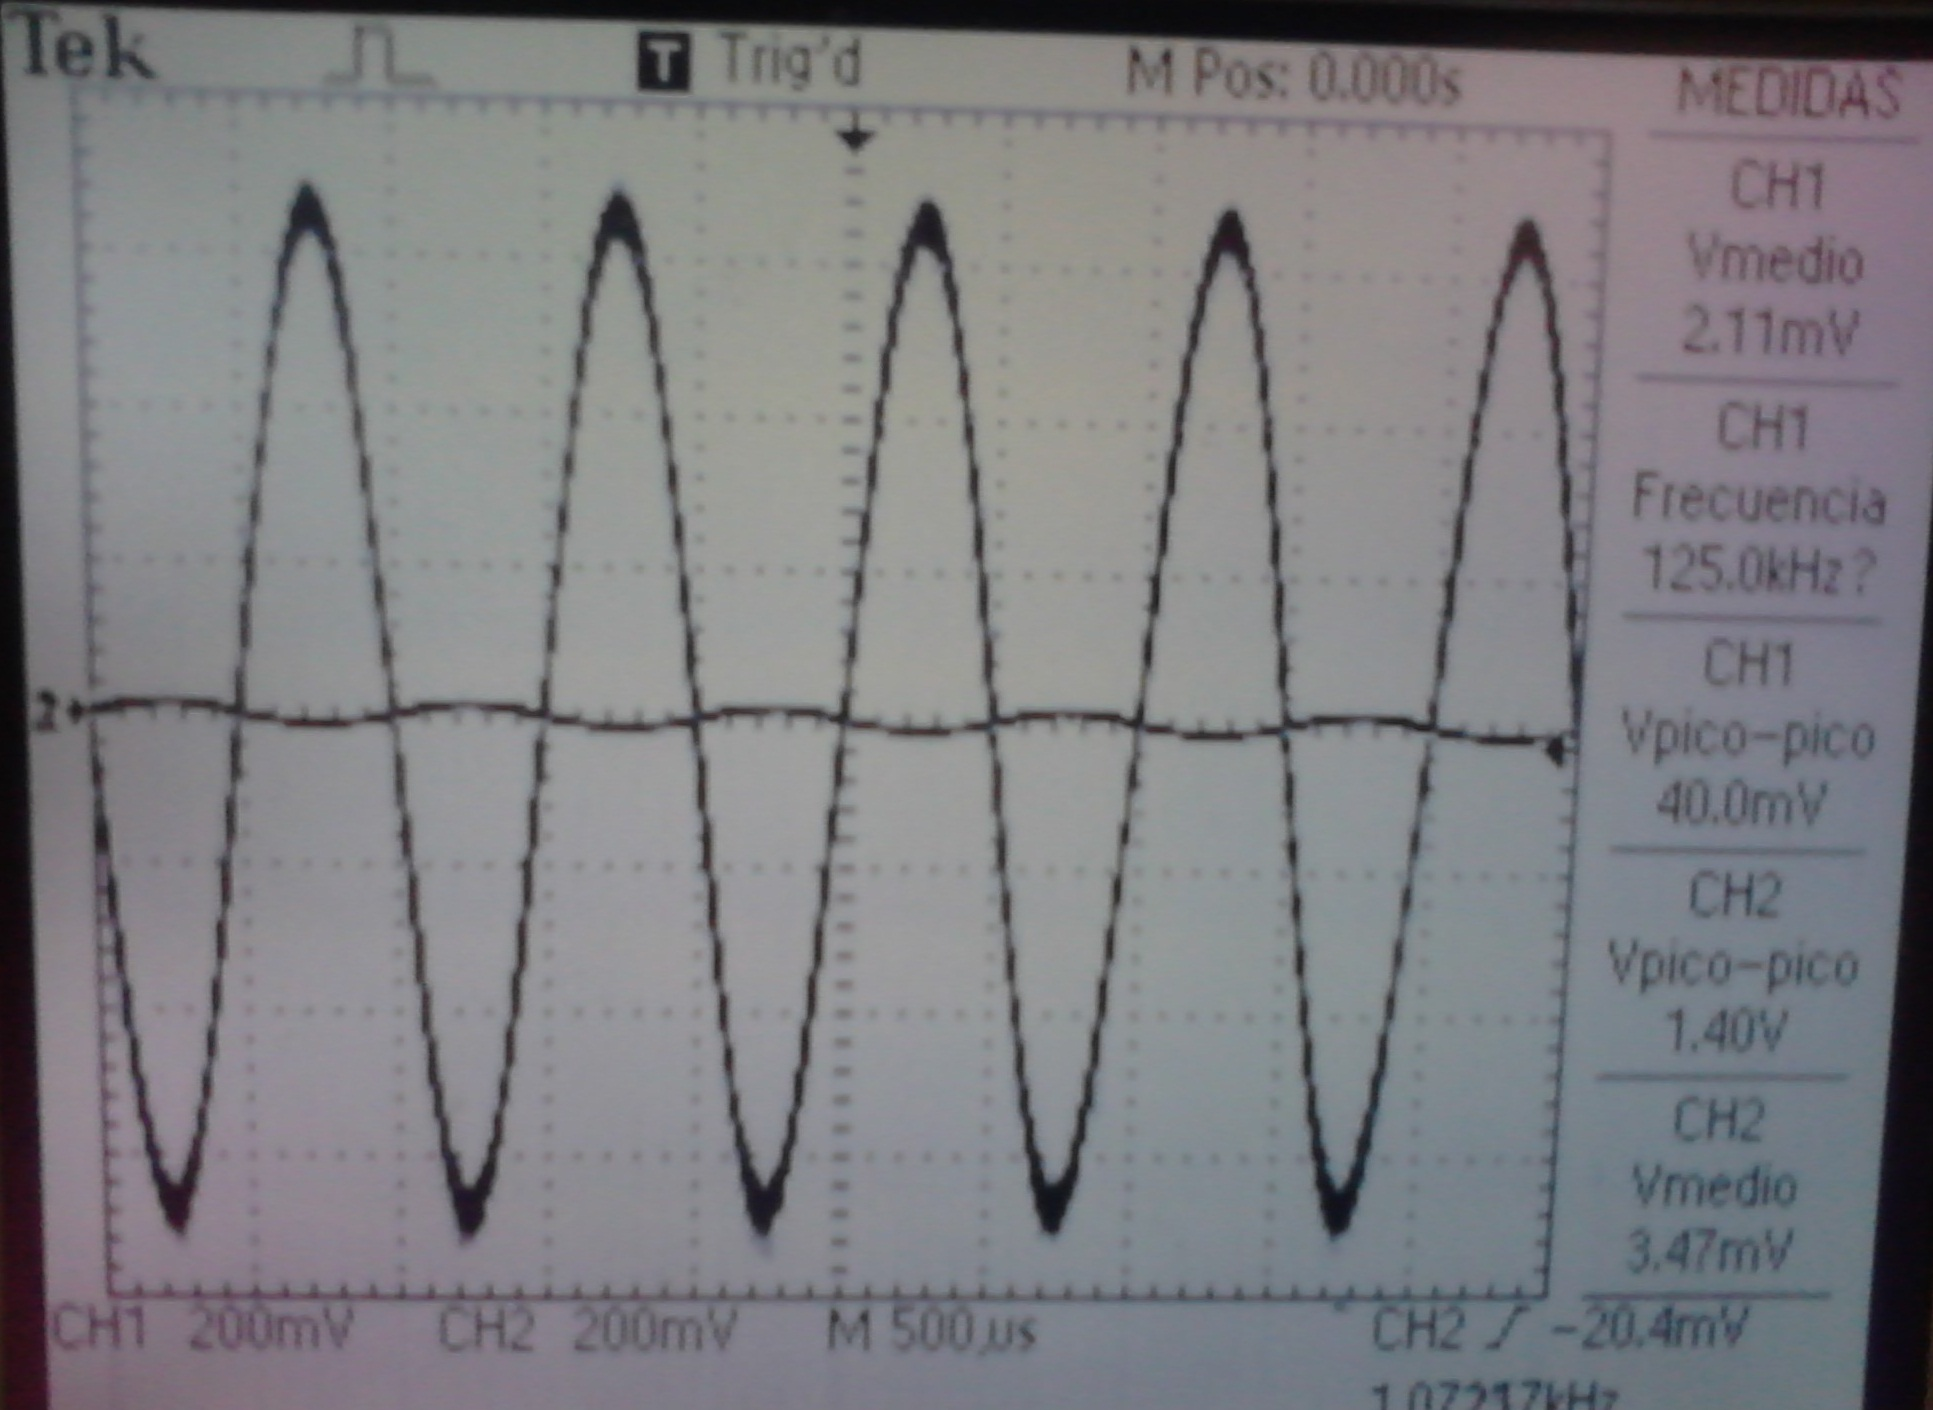
\includegraphics[scale=0.12]{mediciones/3_acoplado_Av.jpg}
\caption{Señal de entrada (CH1) y señal de salida (CH2) medidas con osciloscopio}
\label{fig:B_medicion_Av}
\end{figure}

\subsubsection{Resistencia de entrada}

Se utilizó el banco de medición mostrado en la figura \ref{fig:B_banco_Ri}.
Calculando la diferencia de tensión medida en los dos canales, se mide
la tensión entre los terminales del resistor de $R_p = 47\,\unit{k\Omega}$ para
obtener la corriente y así calcular la resistencia de entrada con la tensión
medida con la punta CH2.

En la figura \ref{fig:B_medicion_Ri} se muestra el resultado obtenido en el osciloscopio
para una señal de entrada de $720\,\unit{mV}$ pico-pico a una frecuencia de
$1\,\unit{kHz}$.

Se calcula $R_i$ mediante:

\[ \displaystyle R_i = \frac{V_{CH2_{max}}}{V_{CH1_{max}} - V_{CH2_{max}}} R_p = 
\frac{224\,\unit{mV}}{364\,\unit{mV} - 224\,\unit{mV}} 47\,\unit{k\Omega} = 
75.2\,\unit{k\Omega}\]

\begin{figure}[H]
\centering
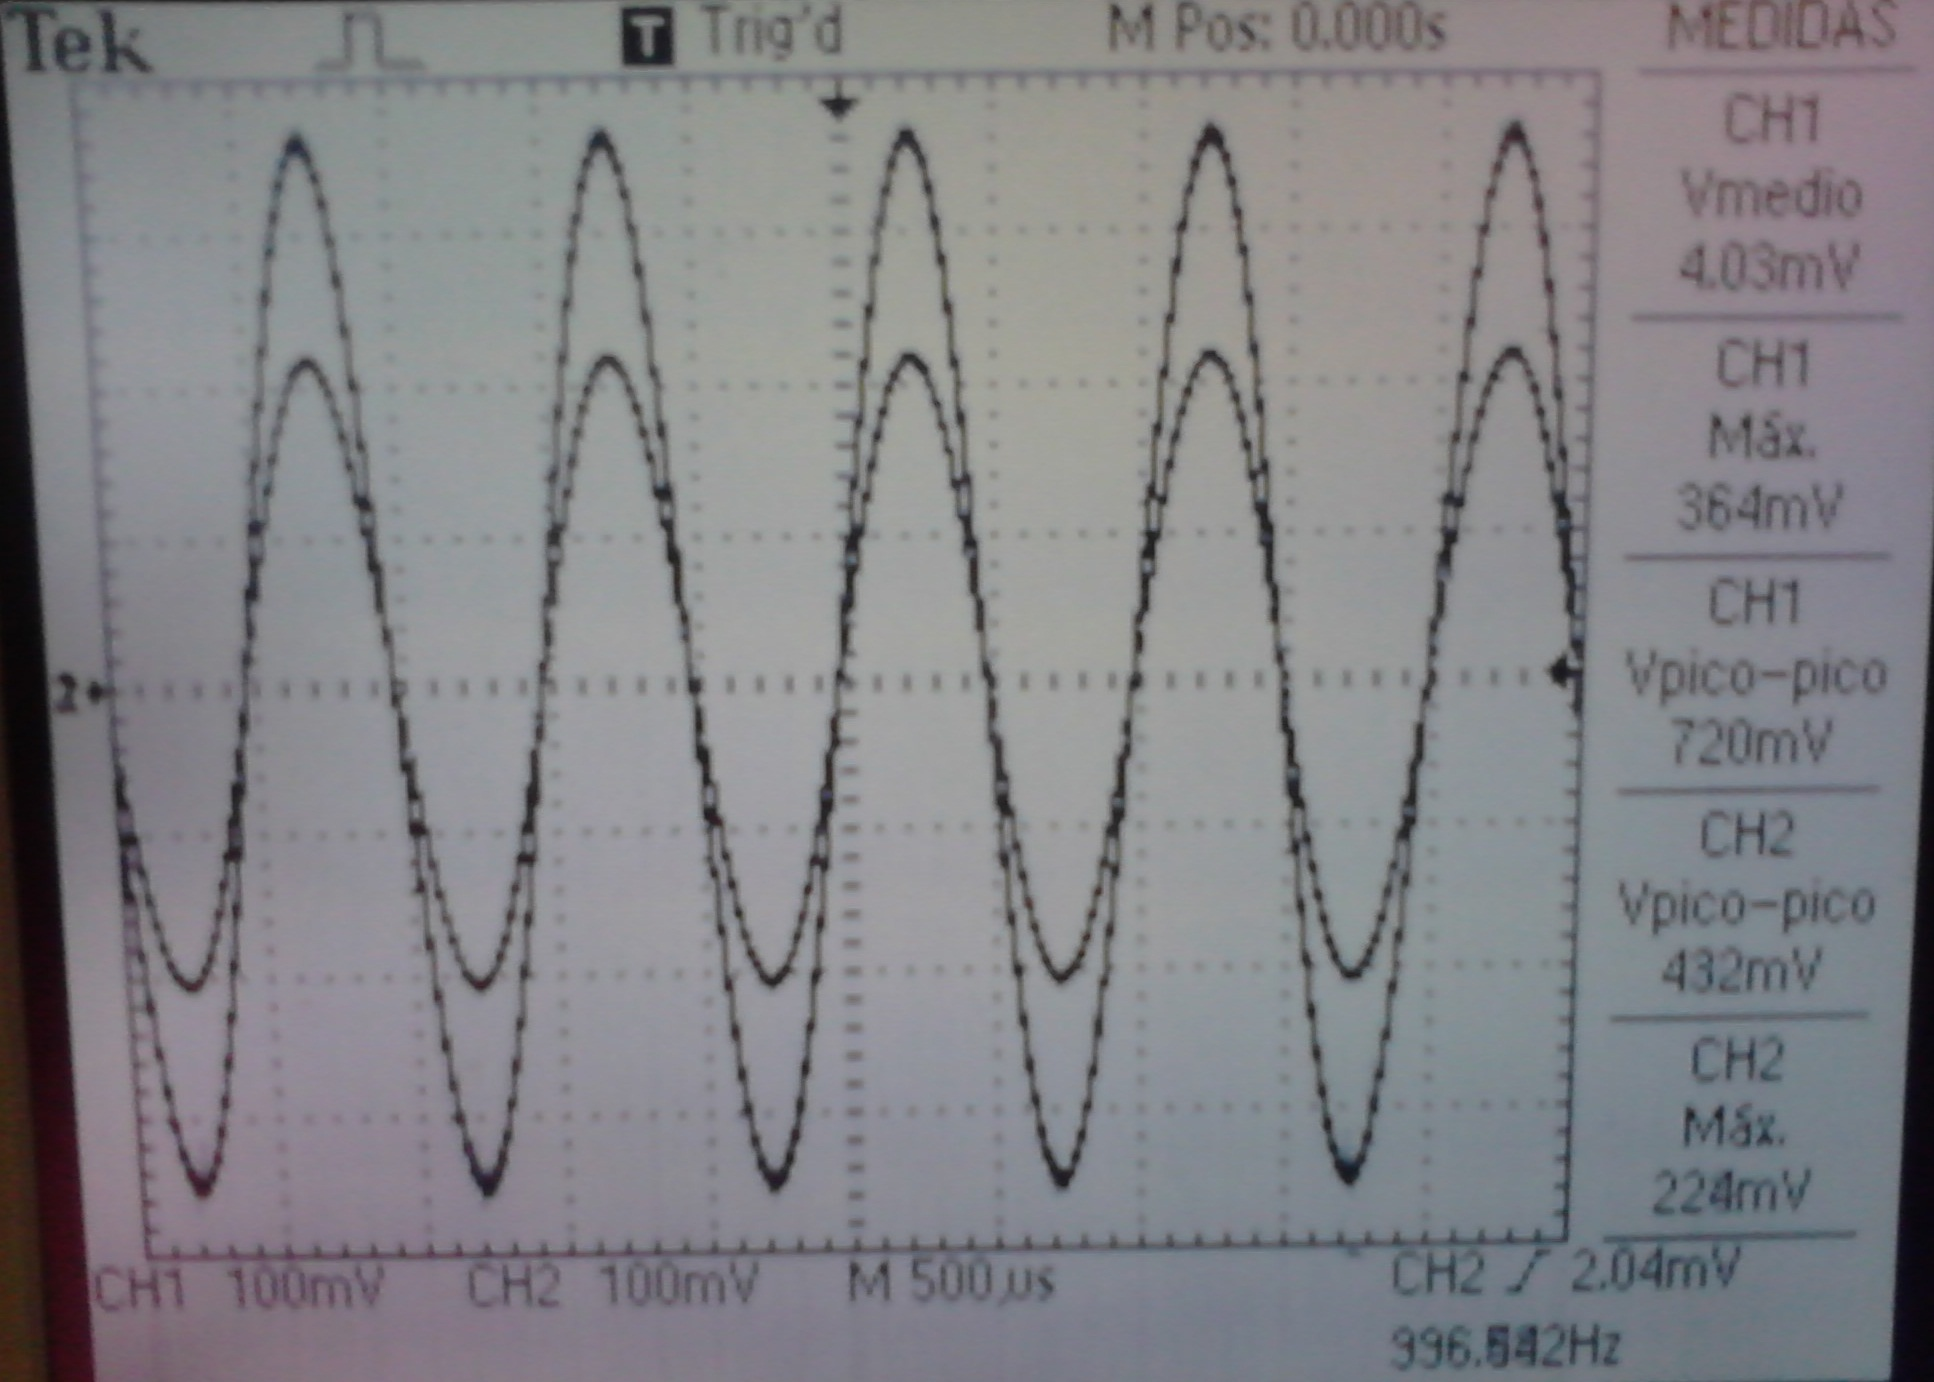
\includegraphics[scale=0.12]{mediciones/3_acoplado_Ri.jpg}
\caption{Señal del generador (CH1) y señal sobre la entrada del seguidor (CH2)}
\label{fig:B_medicion_Ri}
\end{figure}

\subsubsection{Resistencia de salida}

Se utilizó el banco de medición mostrado en la figura \ref{fig:B_banco_Ro}.
Al igual que para $R_i$ se calcula la corriente con la diferencia de tensión
entre el resistor $R_p = 4.7\,\unit{k\Omega}$ y luego calcular la resistencia
de salida en base a la tensión medida por la punta CH2.

En la figura \ref{fig:B_medicion_Ro} se muestra el resultado obtenido en el osciloscopio
para una señal de entrada de $720\,\unit{mV}$ pico-pico a una frecuencia de
$1\,\unit{kHz}$.

Se calcula $R_i$ mediante:

\[ \displaystyle R_o = \frac{V_{CH2_{max}}}{V_{CH1_{max}} - V_{CH2_{max}}} R_p = 
\frac{184\,\unit{mV}}{364\,\unit{mV} - 184\,\unit{mV}} 4.7\,\unit{k\Omega} \approx 
4.8\,\unit{k\Omega}\]

\begin{figure}[H]
\centering
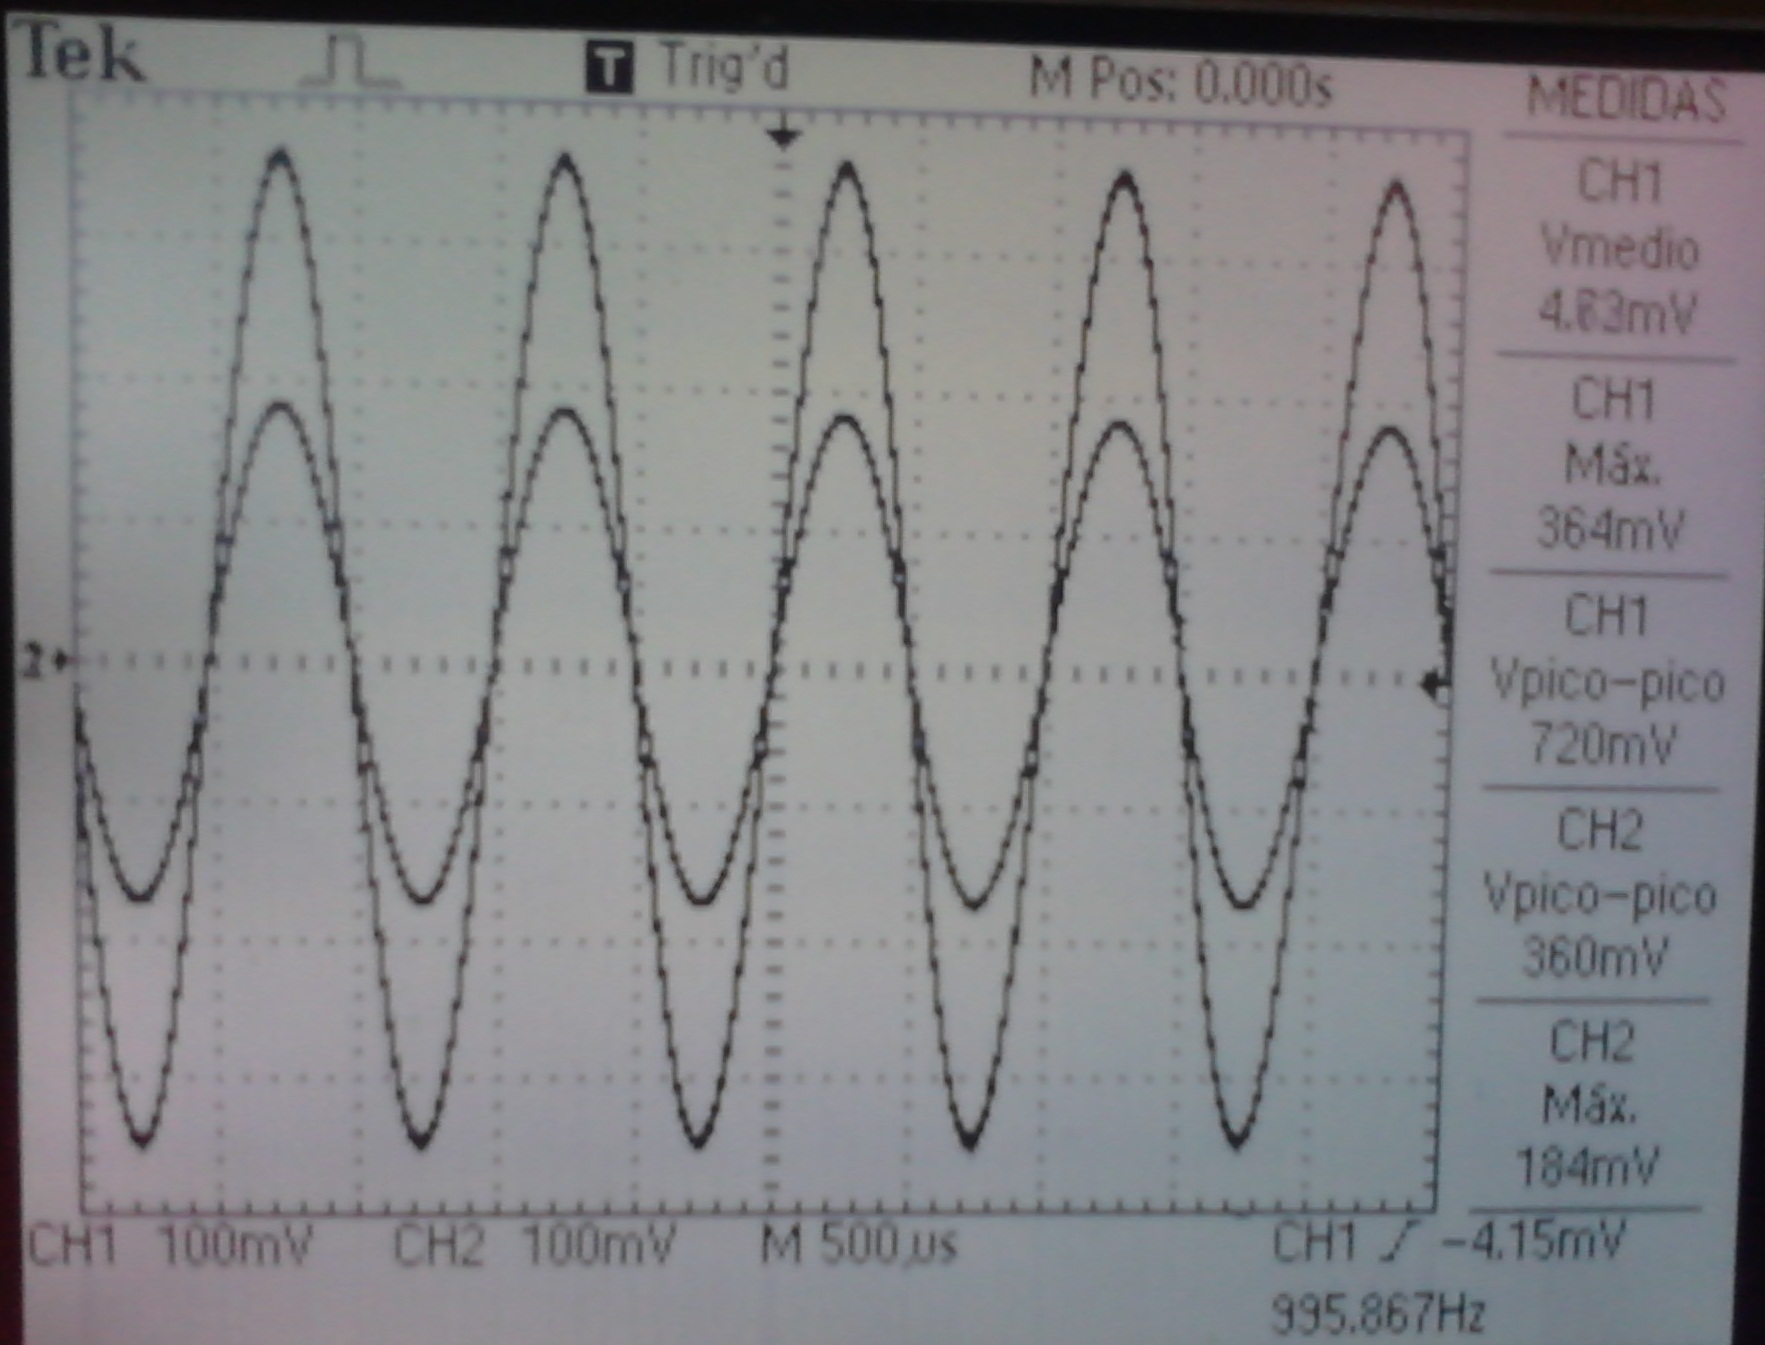
\includegraphics[scale=0.12]{mediciones/3_acoplado_Ro.jpg}
\caption{Señal del generador (CH1) y señal sobre la salida del amplificador (CH2)}
\label{fig:B_medicion_Ro}
\end{figure}

\subsection{Comparación de resultados}

\subsubsection{Punto de reposo de la etapa seguidora}

En la tabla \ref{table:B_comparacion_Q1} se muestra el punto de reposo
Q1 correspondiente a la etapa seguidora del circuito para los distintos
métodos utilizados. Se utilizaron los valores típicos para la columna
correspondiente a los cálculos y simulación.

\begin{table}[H]
\centering
\begin{tabular}{|c|c|c|c|} %aca pones la cantidad de columnas, te faltaba 1. la c indica que esta centrado el dato en su celda y las | son cada linea vertical de la tabla
\hline
Método & Cálculo &  Simulación & Medición \\ \hline
$I_{D1}$ & $4.14\,\unit{mA}$  &  $4.42\,\unit{mA}$ & $4.85\,\unit{mA}$   \\ \hline
$V_{G1}$ & $6.51\,\unit{V}$ & $6.51\,\unit{V}$  &  $6.02\,\unit{V}$  \\ \hline
$V_{D1}$ & $28.0\,\unit{V}$ & $28.0\,\unit{V}$  &  $28.0\,\unit{V}$  \\ \hline
$V_{S1}$ & $4.14\,\unit{V}$ & $4.42\,\unit{V}$  &  $4.85\,\unit{V}$  \\ \hline
$V_{DS1}$ & $23.9\,\unit{V}$ & $23.6\,\unit{V}$  &  $23.15\,\unit{V}$  \\ \hline
$V_{GS1}$ & $2.36\,\unit{V}$ & $2.09\,\unit{V}$ & $1.17\,\unit{V}$  \\ \hline
\end{tabular}
\caption{Tabla comparativa de los puntos Q1 obtenidos mediante diferentes métodos}
\label{table:B_comparacion_Q1}
\end{table}

En la tabla \ref{table:B_errores_Q1} se muestran los errores respecto al valor medido
del punto de reposo Q2 de los valores obtenidos mediante cálculo y simulación.
Para todos los valores se encontró menor error en los resultados obtenidos
mediante las simulaciones en \emph{Spice}.

\begin{table}[H]
\centering
\begin{tabular}{|c|c|c|} %aca pones la cantidad de columnas, te faltaba 1. la c indica que esta centrado el dato en su celda y las | son cada linea vertical de la tabla
\hline
Método & Cálculo &  Simulación  \\ \hline
$I_{D1}$ & -14.6\%  & -8.86\%  \\ \hline
$V_{G1}$ & 8.14\% & 8.14\% \\ \hline
$V_{D1}$ & 0\% & 0\%  \\ \hline
$V_{S1}$ & -14.6\% & -8.87\%  \\ \hline
$V_{DS1}$ & 3.24\% & 1.94\%  \\ \hline
$V_{GS1}$ & 102\% & 102\%  \\ \hline
\end{tabular}
\caption{Tabla con los errores respecto a la medición del punto de reposo Q1}
\label{table:B_errores_Q1}
\end{table}

También se verificó si los valores medidos estan dentro del rango de valores
posibles considerando una dispersión del $30\%$ de los parámetros $V_T$ y $K$.

En la tabla \ref{table:B_Q1_rango} se muestran los rangos de valores obtenidos
mediante cálculo por inspección y simulación junto a los valores medidos.

De la tabla se puede obsevar que los valores medidos están fuera de los rangos
de valores obtenidos. Esto se debe a que se consideró una dispersión del $30\%$
de los parámetros $V_T$ y $K$. Sin embargo los valores medidos son muy cercanos
a los valores máximos obtenidos en cada método, considerando $V_T = 1.47\,\unit{V}$ y 
$K = 160\,\unit{\frac{mA}{V^2}}$.
Para evitar esto se debería considerar la dispersión máxima y mínima de los
parámetros según las hojas de datos, $V_{T_{min}} = 0.8\,\unit{V}$ y $V_{T_{max}} = 3\,\unit{V}$,
en lugar del $30\%$ respecto al valor tipico.


\begin{table}[H]
\centering
\begin{tabular}{|c|c|c||c|} %aca pones la cantidad de columnas, te faltaba 1. la c indica que esta centrado el dato en su celda y las | son cada linea vertical de la tabla
\hline
Método & Cálculo &  Simulación & Medición 
\\ \hline
$I_{D1}$ & [ $3.49\,\unit{mA}$ ; $4.79\,\unit{mA}$ ]  &  [ $3.49\,\unit{mA}$ ; $4.79\,\unit{mA}$ ] & $4.85\,\unit{mA}$
\\ \hline
$V_{G1}$ & [ $6.51\,\unit{V}$ ; $6.51\,\unit{V}$ ] & [ $6.51\,\unit{V}$ ; $6.51\,\unit{V}$ ] & $6.02\,\unit{V}$  
\\ \hline
$V_{D1}$ & [ $28\,\unit{V}$ ; $28\,\unit{V}$ ] & [ $28\,\unit{V}$ ; $28\,\unit{V}$ ] & $28\,\unit{V}$  
\\ \hline
$V_{S1}$ & [ $3.49\,\unit{V}$ ; $4.79\,\unit{V}$ ] & [ $3.49\,\unit{V}$ ; $4.79\,\unit{V}$ ] & $4.85\,\unit{V}$  
\\ \hline
$V_{DS1}$ & [ $23.2\,\unit{V}$ ; $24.5\,\unit{V}$ ] & [ $23.1\,\unit{V}$ ; $24.5\,\unit{V}$ ] & $23.15\,\unit{V}$  
\\ \hline
$V_{GS1}$ & [ $1.71\,\unit{V}$ ; $3.01\,\unit{V}$ ] & [ $1.72\,\unit{V}$ ; $3.02\,\unit{V}$ ] & $1.17\,\unit{V}$  
\\ \hline
\end{tabular}
\caption{Tabla del punto de reposo Q1 medido y el rango de valores obtenido mediante cálculo y medición}
\label{table:B_Q1_rango}
\end{table}

\subsubsection{Punto de reposo de la etapa amplificadora}

En la tabla \ref{table:B_comparacion_Q2} se muestra el punto de reposo
Q2 correspondiente a la etapa amplificadora del circuito para los distintos
métodos utilizados. Se utilizaron los valores típicos para la columna
correspondiente a los cálculos y simulación.

\begin{table}[H]
\centering
\begin{tabular}{|c|c|c|c|} %aca pones la cantidad de columnas, te faltaba 1. la c indica que esta centrado el dato en su celda y las | son cada linea vertical de la tabla
\hline
Método & Cálculo &  Simulación & Medición \\ \hline
$I_{D2}$ & $1.87\,\unit{mA}$  &  $2.40\,\unit{mA}$ & $3.31\,\unit{mA}$   \\ \hline
$V_{G2}$ & $4.14\,\unit{V}$ & $4.42\,\unit{V}$  &  $4.85\,\unit{V}$  \\ \hline
$V_{D2}$ & $19.1\,\unit{V}$ & $16.7\,\unit{V}$  &  $12.5\,\unit{V}$  \\ \hline
$V_{S2}$ & $1.87\,\unit{V}$ & $2.4\,\unit{V}$  &  $3.31\,\unit{V}$  \\ \hline
$V_{DS2}$ & $17.2\,\unit{V}$ & $14.3\,\unit{V}$  &  $9.15\,\unit{V}$  \\ \hline
$V_{GS2}$ & $2.27\,\unit{V}$ & $2.02\,\unit{V}$ & $1.54\,\unit{V}$  \\ \hline
\end{tabular}
\caption{Tabla comparativa de los puntos Q2 obtenidos mediante diferentes métodos}
\label{table:B_comparacion_Q2}
\end{table}

En la tabla \ref{table:B_errores_Q2} se muestran los e rrores respecto al valor medido
del punto de reposo Q2 de los valores obtenidos mediante cálculo y simulación.
Para todos los valores se encontró menor error en los resultados obtenidos
mediante las simulaciones en \emph{Spice}.


\begin{table}[H]
\centering
\begin{tabular}{|c|c|c|} %aca pones la cantidad de columnas, te faltaba 1. la c indica que esta centrado el dato en su celda y las | son cada linea vertical de la tabla
\hline
Método & Cálculo &  Simulación  \\ \hline
$I_{D2}$ & -43.5\%  & -27.5\%  \\ \hline
$V_{G2}$ & 14.6\% & 8.87\% \\ \hline
$V_{D2}$ & 52.8\% & 33.6\%  \\ \hline
$V_{S2}$ & -43.5\% & -27.5\%  \\ \hline
$V_{DS2}$ & 88.0\% & 56.3\%  \\ \hline
$V_{GS2}$ & 47.4\% & 31.2\%  \\ \hline
\end{tabular}
\caption{Tabla con los errores respecto a la medición del punto de reposo Q2}
\label{table:B_errores_Q2}
\end{table}


Se verificó si los valores medidos están dentro del rango de valores
posibles considerando una dispersión del $30\%$ de los parámetros $V_T$ y $K$.

En la tabla \ref{table:B_Q2_rango} se muestran los rangos de valores obtenidos
mediante cálculo por inspección y simulación junto a los valores medidos.

Al igual que para el seguidor se puede observar que los valores medidos están fuera de los rangos
de valores calculados y simulados. Debido a no haber tomado una dispersión del mínimo y máximo
$V_T$ en lugar de tomar una dispersión del $30\%$.

También se observa que los valores medidos son muy cercanos
a los valores máximos obtenidos en cada método, considerando $V_T = 1.47\,\unit{V}$ y 
$K = 160\,\unit{\frac{mA}{V^2}}$.


\begin{table}[H]
\centering
\begin{tabular}{|c|c|c||c|} %aca pones la cantidad de columnas, te faltaba 1. la c indica que esta centrado el dato en su celda y las | son cada linea vertical de la tabla
\hline
Método & Cálculo &  Simulación & Medición 
\\ \hline
$I_{D2}$ & [ $640\,\unit{\mu A}$ ; $3.12\,\unit{mA}$ ]  &  [ $638\,\unit{\mu A}$ ; $3.12\,\unit{mA}$ ] & $3.31\,\unit{mA}$
\\ \hline
$V_{G2}$ & [ $3.49\,\unit{V}$ ; $4.79\,\unit{V}$ ] & [ $3.49\,\unit{V}$ ; $4.79\,\unit{V}$ ] & $4.85\,\unit{V}$ 
\\ \hline
$V_{D2}$ & [ $13.3\,\unit{V}$ ; $25.0\,\unit{V}$ ] & [ $13.3\,\unit{V}$ ; $25.0\,\unit{V}$ ] & $12.46\,\unit{V}$  
\\ \hline
$V_{S2}$ & [ $640\,\unit{mV}$ ; $3.12\,\unit{V}$ ] & [ $638\,\unit{mV}$ ; $3.12\,\unit{V}$ ] & $3.31\,\unit{V}$  
\\ \hline
$V_{DS2}$ & [ $10.2\,\unit{V}$ ; $24.4\,\unit{V}$ ] & [ $10.2\,\unit{V}$ ; $24.4\,\unit{V}$ ] & $9.15\,\unit{V}$  
\\ \hline
$V_{GS2}$ & [ $1.67\,\unit{V}$ ; $2.85\,\unit{V}$ ] & [ $1.67\,\unit{V}$ ; $2.85\,\unit{V}$ ] & $1.54\,\unit{V}$  
\\ \hline
\end{tabular}
\caption{Tabla del punto de reposo Q2 medido y el rango de valores obtenido mediante cálculo y medición}
\label{table:B_Q2_rango}
\end{table}


\subsubsection{Parámetros del circuito}

En la tabla \ref{table:B_comparacion_parametros} se muestran los parámetros
del circuito amplificador acoplado a una etapa seguidora obtenidos mediante
distintos métodos.

Se realiza una comparación del error que se comete al obtener los parámetros
mediante cálculo por inspección y simulación respecto a la medición. En la
tabla \ref{table:B_error_parametros} se pueden ver los errores obtenidos.
No se encontraron diferencias significativas entre los errores obtenidos
por ambos métodos.

\begin{table}[H]
\centering
\begin{tabular}{|c|c|c|c|} %aca pones la cantidad de columnas, te faltaba 1. la c indica que esta centrado el dato en su celda y las | son cada linea vertical de la tabla
\hline
Método & $A_v$ & $R_i$  & $R_o$ \\ \hline
Teórico & -43.5 & $89\,\unit{k\Omega}$  & $4.7\,\unit{k\Omega}$   \\ \hline
Simulación & -45 & $80\,\unit{k\Omega}$  & $4.5\,\unit{k\Omega}$   \\ \hline
Medición & -20 & $84\,\unit{k\Omega}$  & $5\,\unit{k\Omega}$   \\ \hline
\end{tabular}
\caption{Tabla con los parametros obtenidos a $1\,\unit{k\ Hz}$ mediante diferentes métodos}
\label{table:B_comparacion_parametros}
\end{table}


\begin{table}[H]
\centering
\begin{tabular}{|c|c|c|c|} %aca pones la cantidad de columnas, te faltaba 1. la c indica que esta centrado el dato en su celda y las | son cada linea vertical de la tabla
\hline
Método & $A_v$ & $R_i$  & $R_o$ \\ \hline
Teórico & 117\% & 6\%  & -6\%  \\ \hline
Simulación & 125\% & -5\%  & -10\%  \\ \hline
\end{tabular}
\caption{Tabla con los errores de los parametros obtenidos respecto a la medición}
\label{table:B_error_parametros}
\end{table}

En la tabla \ref{table:B_rango_Av} se compara el valor medido de $A_v$ con los rangos de valores de $A_v$
medidos y simulados. Para verificar si el valor medido se encuentra dentro del rango de valores.

Se observa que el valor de $A_v$ medido está dentro del rango de valores calculados y simulados.
Sin embargo se encuentra muy cercano al caso extremo planteado en el que $V_T = 2.73\,\unit{V}$ y 
$K = 123\,\unit{\frac{mA}{V^2}}$.

\begin{table}[H]
\centering
\begin{tabular}{|c|c|c||c|} %aca pones la cantidad de columnas, te faltaba 1. la c indica que esta centrado el dato en su celda y las | son cada linea vertical de la tabla
\hline
Método & Cálculo &  Simulación & Medición 
\\ \hline
$A_{v}$ & [ -119 ; -31.7 ]  &  [ -95 ; -31 ] & -35
\\ \hline
\end{tabular}
\caption{Tabla de la amplificación medida y rangos obtenidos mediante cálculo y simulación}
\label{table:B_rango_Av}
\end{table}



\subsection{Preguntas}

{\color{OliveGreen} 
¿Cómo se modifica el equivalente de Thévenin del generador que excita a la etapa
amplificadora original cuando se agrega la etapa seguidor?
}\\

Los circuitos seguidores tienen amplificaciones menores que 1. Por lo que
agregar un circuito seguidor a la salida del generador sería equivalente a
aumentar la resistencia del equivalente de Thévenin del generador que
excita a la etapa amplificadora.

Considerando que la resistencia interna de la etapa amplificadora $R_i = 89\,\unit{k\Omega}$
Observando el circuito de la figura \ref{fig:B_pregunta_thevenin} 
se deduce que para llegar al mismo efecto que la etapa seguidora
de reducir a 0.96 veces la señal de entrada, se debe obtener
la misma proporción de $v_i$ en el divisor resistivo formado por
$R_{Thevenin}$ y $R_i$.

Entonces se plantea:

\[ \displaystyle A_{v1} = \frac{R_i}{R_i + R_{Thevenin}} \]

Se despeja y calcula $R_{Thevenin}$:

\[ \displaystyle R_{Thevenin} = R_i \frac{1-A_v}{A_v} =
89\,\unit{k\Omega} \frac{1-0.96}{0.96} \approx 3.7\,\unit{k\Omega}\]

\begin{figure}[H]
\centering
\begin{circuitikz}[]\shorthandoff{>}
\draw 
(0,0) to [sV, l=$V_{Thevenin}$] (0,3)
to [R, l=$R_{Thevenin}$] (3,3)
to [R, l=$R_i$] (3,0)
to [short, -*] (1.5,0)
to [short] (0,0)
(1.5,0) node[ground]{}
(3,3) to [short, *-o] (3.5,3) node[anchor=south] {$v_i$}

;\end{circuitikz}
\caption{Equivalente de Thévenin del la tensión de entrada del amplificador}
\label{fig:B_pregunta_thevenin}
\end{figure}


{\color{OliveGreen}
¿Cómo son los nuevos parámetros $R_i$, $R_o$ y $A_v$ de esta etapa con dos
transistores respecto a los obtenidos en la etapa original bajo estudio?
}\\

En la tabla \ref{table:comparacion_seguidor} se muestran los parámetros
con y sin etapa seguidora obtenidos mediante cálculos por inspección.

\begin{table}[H]
\centering
\begin{tabular}{|c|c|c|} 
\hline
Parámetro & Sin seguidor & Con seguidor \\ \hline 
$A_v$ & -43.5 & -64 \\ \hline 
$R_i$ & $89\,\unit{k\Omega}$ & $76.7\,\unit{k\Omega}$ \\ \hline
$R_o$ & $4.70\,\unit{k\Omega}$ & $4.70\,\unit{k\Omega}$ \\ \hline 
\end{tabular}
\caption{Tabla comparativa de las caracteristicas del amplificadr con y sin etapa seguidora.}
\label{table:comparacion_seguidor}
\end{table}


En base a los resultados obtenidos se observa que la amplificación $A_v$
aumenta respecto al amplificador sin etapa seguidora.
Esto se debe a que no se pudo mantener el mismo punto $Q2$ de la
etapa amplificadora acoplada directamente al seguidor. 
Ya que el la etapa seguidora es la encargada de polarizar a
la etapa amplificadora, y por estar limitados a los valores normalizados
de resistencias no se pudo obtener el mismo punto $Q2$ sin seguidor.
Sin etapa seguidora para valores típicos se obtiene $V_{GS2} = 1.95\,\unit{V}$ y con etapa seguidora se obtiene $V_{GS2} = 2.02\,\unit{V}$. Al aumentar $V_{GS2}$ aumenta $g_{m2}$.
Y al aumentar $g_{m2}$ aumenta $A_{v2}$.

Se observa que al agregar la etapa seguidora se modifica la resistencia interna
$R_i$, ya que ahora esta depende del circuito seguidor. Se utilizaron
valores elevados para las resistencias de polarización de la etapa seguidora
para intentar mantener la resistencia de entrada alta de la etapa amplificadora.
Sin embargo no se logró mantener exactamente el mismo valor ya que también
se debieron elegir los valores adecuados de resistencias para que la etapa
seguidora pueda polarizar a la etapa amplificadora adecuadamente.

No se observan cambios en $R_o$ ya que este depende solo de la resistencia
$R_D$ del amplificador.

\section{Oscilador senoidal por desplazamiento de fase}

\subsection{Circuito simulado}

En la figura \ref{fig:5_oscilador} se muestra el circuito propuesto 
del oscilador.

\begin{figure}[H]
\centering
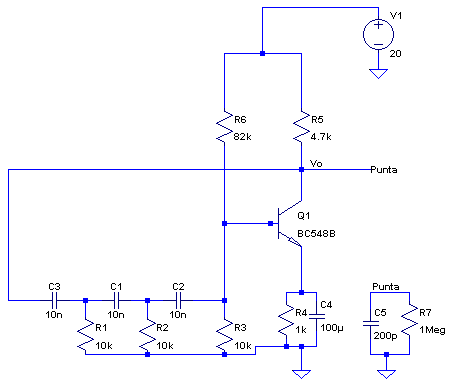
\includegraphics[scale=0.75]{circuitos/5_oscilador.png}
\caption{Circuito para simular el oscilador}
\label{fig:5_oscilador}
\end{figure}

Se obtuvo la respuesta mostrada en la figura \ref{fig:5_salida} a partir de la simulación en \emph{Spice}.

\begin{figure}[H]
\centering
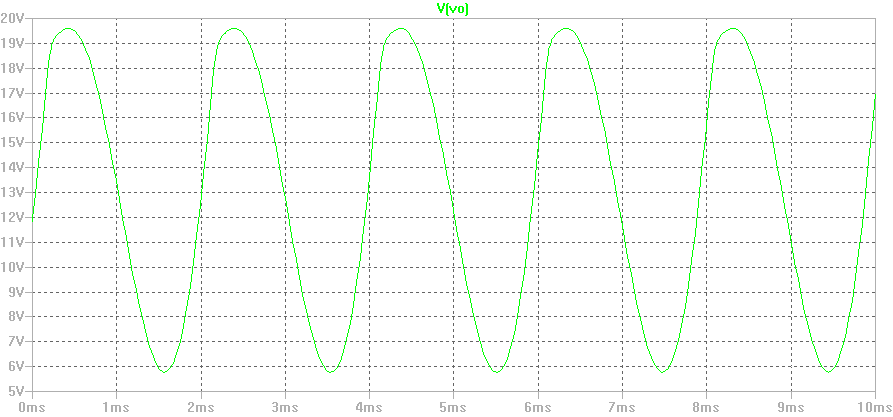
\includegraphics[scale=0.4]{simulaciones/5_salida.png}
\caption{Salida simulada del oscilador}
\label{fig:5_salida}
\end{figure}



\subsection{Preguntas}


{\color{OliveGreen} 
Explicar cualitativamente por qué la señal $v_o$ resulta ser
periódica (forma cuasi senoidal). Utilizar los conceptos generales de
realimentación para demostrar, recorriendo el lazo, que la realimentación es
positiva.}
\\

Conociendo la salida del amplificador ``emisor común", sabemos que el desfasaje
entre la entrada y la salida es de 180 grados.
Si a este amplificador, se le agrega una red RC como realimentación esta tendrá un
desfasaje adicional. Por lo tanto, agregando 3 redes RC, se consigue un desfasaje
de 180 grados.
Si se suman ambos desfasajes en frecuencias muy altas, se llega a los 360 grados, o en otras palabras, se
vuelve a cero, sumando tensión en valores positivos de entrada y restando en
valores negativos. Pero debido al retardo del circuito para producir los cambios
mediante la realimentación, los valores realimentados hacen oscilar la salida en
vez de estabilizarla.

Al recorrer la malla de realimentación, se busca que $|A_0.\beta|=1$, 
donde $A_0=\frac{V_o}{V_i}$ y $\beta=\frac{V_c}{V_o}$. 
Esto se debe a que, valores menores de realimentación harán 
que la señal se atenue hasta llegar a cero, y
valores mayores la harán crecer hasta los valores de alimentación, 
dejando de ser un oscilador útil.
\\

{\color{OliveGreen} 
Sin obtener una expresión analítica, justificar a partir del
análisis del comportamiento de la realimentación, cómo se relaciona
aproximadamente la frecuencia de la señal $v_0$ con los valores de la red RC.}
\\

Realizando un análisis cualitativo del circuitos, se puede pensar en el diagrama
de Bode de una de las redes RC de realimentación. Se sabe que a partir de una
determinada frecuencia $f_0$, la fase se modificará en 90 grados.
Para esta red se sabe también que

\[ \displaystyle f_0=\frac{1}{2.\pi.\tau} \]
\[ \displaystyle \tau=R.C \]

Utilizando los valores del circuito ($R=10\,\unit{k\Omega}$, $C=10\,\unit{nF}$),
se obtiene una frecuencia de corte

\[\displaystyle f_c=1591.55\,\unit{Hz}\]

Por otro lado, para 3 redes RC, el desfasaje de cada una sera aproximadamente de
60 grados. Por lo que la frecuencia de corte será menor (más a la izquierda en el
diagrama de Bode, teniendo en cuenta la escala logarítmica). Comparando con la
frecuencia de corte obtenida en la simulación ($f_c=500\,\unit{Hz}$), se puede
decir que el calculo aproximado fue bastante cercano.

\subsection{Mediciones}

Durante la etapa de mediciones se utilizaron las placas ofrecidas por el laboratorio. Se noto que al realizar una conexión entre ellas con un cable muy largo, se producia mucho ruido.

Se obtuvo una señal periodica, senoidal, de frecuencia $471.7\,\unit{Hz}$, como se puede ver en la figura \ref{fig:5_salida_med}.

\subsection{Comparación de resultados}

A continuación se analizarán los valores medidos, simulados y calculados. Se puede ver en la tabla \ref{table:5_comparacion_mediciones} que los ordenes de magnitud de las frecuencias de corte son similares (en escala logaritmica) y el error porcentual entre estos valores y el valor medido es muy pequeño.
Sobre la forma de la señal de salida, se puede ver que es una senoidal deformada, tanto en la simulación como en las mediciones. Esto se debe al aporte en menor medida de distinos armonicos, ya que el oscilador no es ideal.


\begin{table}[H]
\centering
\begin{tabular}{|c|c|c|c|} 
\hline

 & Calculo & Simulación & Medición \\ \hline
$f_c$ & $1591.55\,\unit{Hz}$ & $500\,\unit{Hz}$ & $471.7\,\unit{Hz}$\\ \hline
Error & $237.41\%$ & $5.99\%$ & $-$\\ \hline
log($f_c$) & $3.2018$ & $2.6989$ & $2.6736$\\ \hline
Error (log) & $19.75\%$ & $0.95\%$ & $-$ \\ \hline

\end{tabular}
\caption{Comparación de valores calculados, simulados y medidos.}
\label{table:5_comparacion_mediciones}
\end{table}


\begin{figure}[H]
\centering
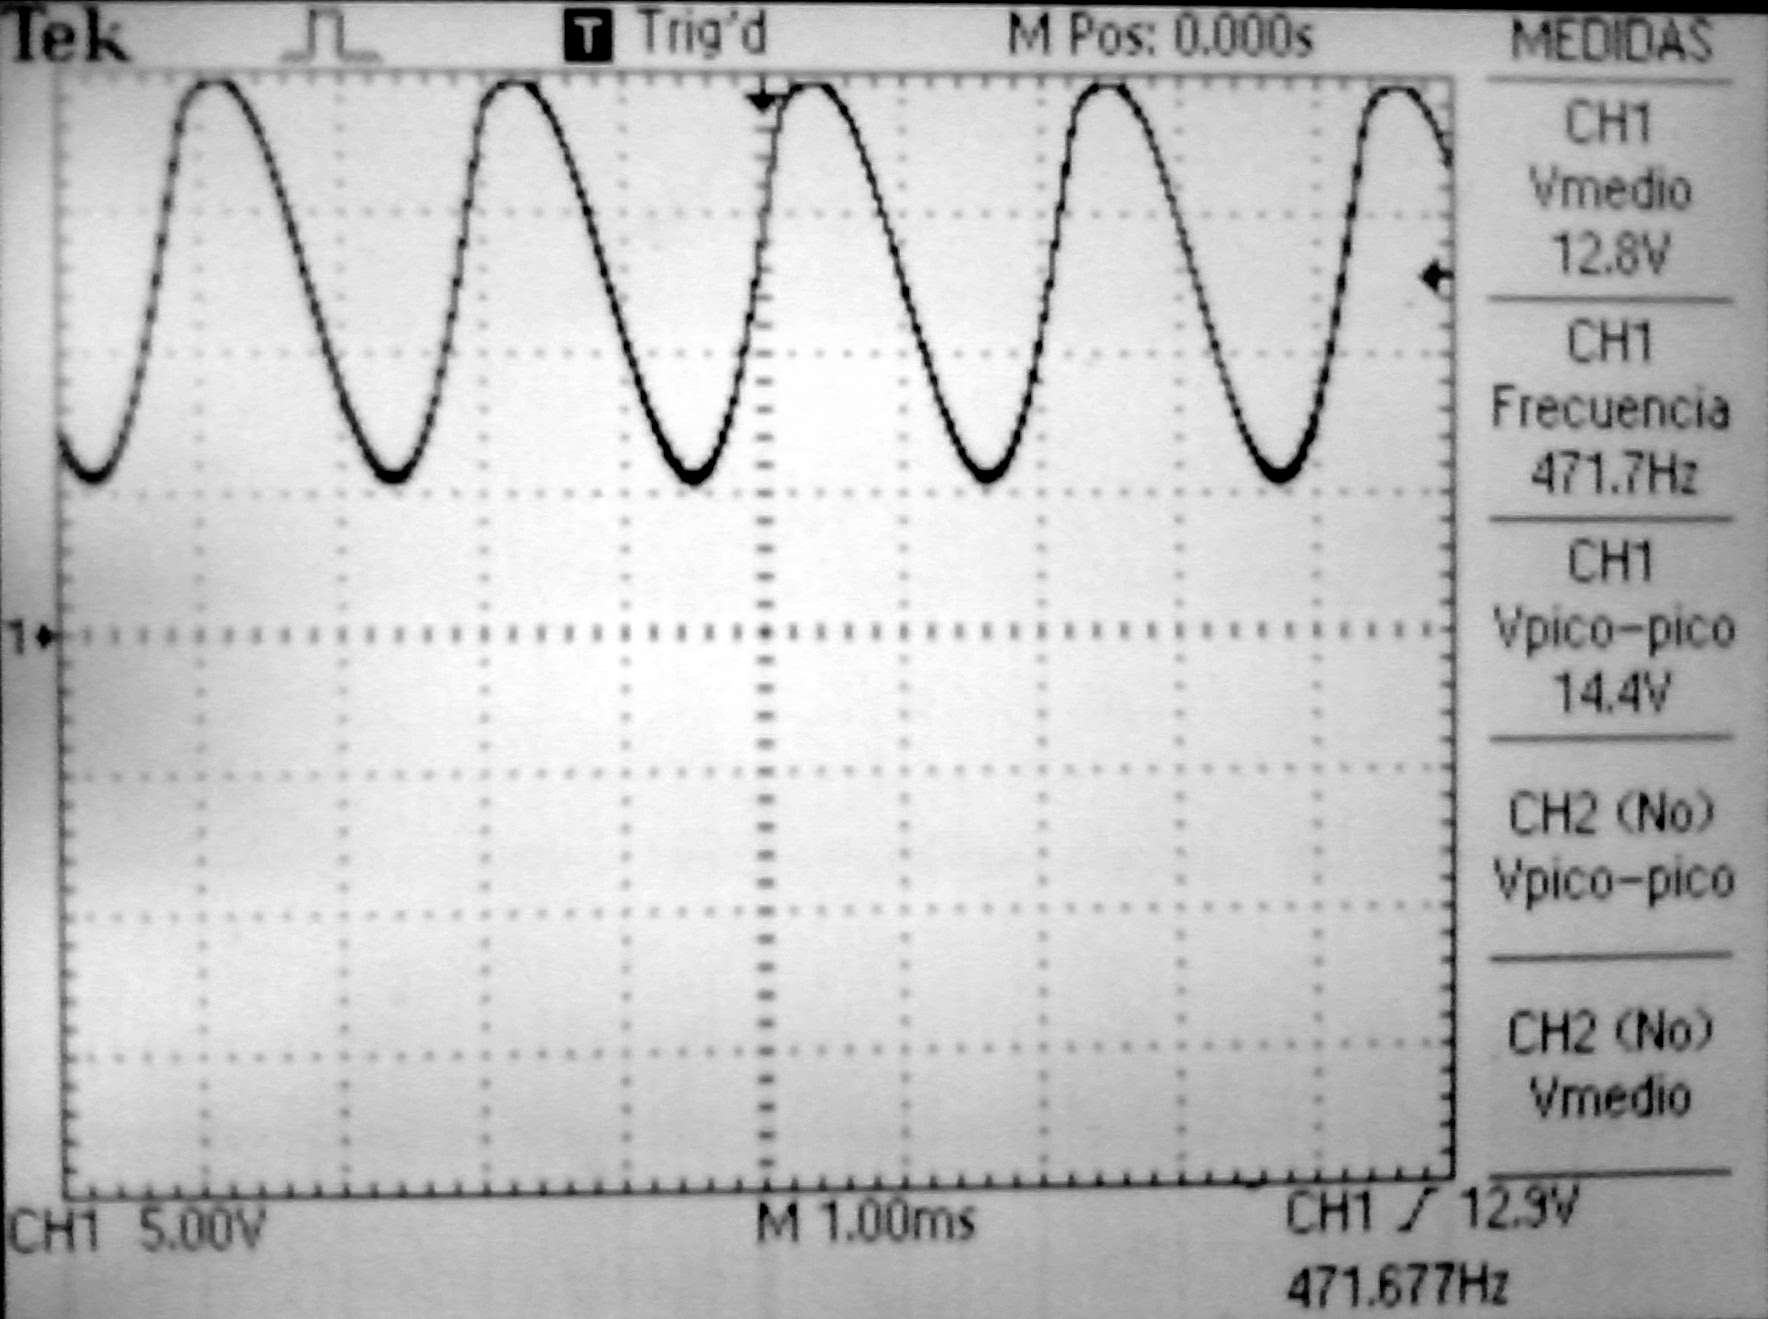
\includegraphics[scale=0.1]{mediciones/5_salida.jpg}
\caption{Salida medida del oscilador}
\label{fig:5_salida_med}
\end{figure}


\section{Conclusiones}

\subsection{Amplificador con un transistor}
De esta etapa se concluye que, si bien se puede usar el modelo teórico para su diseño, es necesario tener en cuenta la variación total de los parametros propios del transistor MOSFET ($k$ y $V_T$), ya que influyen en las caracteristicas que se desean del amplificador (especialmente en la ganancia dentro las tensiones y corrientes que se manejan en este diseño). Se habla de variación total ya que en el analisis realizado se tomó en cuenta una variacion solamete del 30\% y no coincidió con lo medido.

Por otra parte, se vió que existen diferentes criterios para fijar el limite dentro del que el transistor se sigue comportando linealmente. Estos límites pueden ser elegidos para lograr un mayor o menor error de acuerdo a la aplicación que sea necesaria. Estos limites dependen tanto de los parámetros propios del transistor, como de su polarización.

Si se desea obtener una amplificación menos dispersa es necesario realimentar el circuito en señal. Esto reduce drásticamente la amplificación obtenida, pero disminuiría notablemente
su variación. En caso de necesitarse una amplificación elevada se pueden poner varias
etapas de amplificadores realimentados en señal hasta lograr la amplificación deseada.

\subsection{Amplificador con etapa seguidora}

Al igual que para las concluciones del amplificador, es necesario tomar los valores mínimos y máximos
de los parámetros del transistor al analizar la dispersión, ya que tomando una dispersión del 30\% se
obtuvieron valores fuera del rango de valores calculados por inspección y simulados.

Los seguidores resultan utiles para modificar las resistencias de entrada o del amplificador
acoplándolo a la etapa amplificadora.
En caso de contarse con un amplificador que utiliza un transistor TBJ, su resistencia de entrada 
será pequeña debido al valor de $r_{\pi}$ del transistor. Si se desea tener una resistencia de entrada
mayor se puede agregar una etapa seguidora con una resistencia de entrada alta.


\subsection{Oscilador senoidal por desplazamiento de fase}

De la etapa del oscilador concluye que es posible construir un circuito que entregue una señal senoidal de salida, aunque con mucha facilidad esta saldrá deformada. Esto se puede apreciar tanto en las mediciones y la simulación.

Por otro lado, la salida del circuito utilizado posee acoplada una tensión continua, que podría ser eliminada.


\newpage
\begin{thebibliography}{9}

\bibitem{TBJ BC548B}
  \ULurl{http://www.philohome.com/sensors/gp2d12/gp2d12-datasheets/bc548.pdf}

\bibitem{NMOS BS170}
  \ULurl{https://www.fairchildsemi.com/datasheets/BS/BS170.pdf}

\bibitem{JFET 2N5486}
  \ULurl{http://www.onsemi.com/pub_link/Collateral/2N5486-D.PDF}

\end{thebibliography}

\end{document}